\section{Results:}
\subsection{Results using BDRS + Filtering.}
We use the following color convention for graphs through out the document:
\begin{center}
    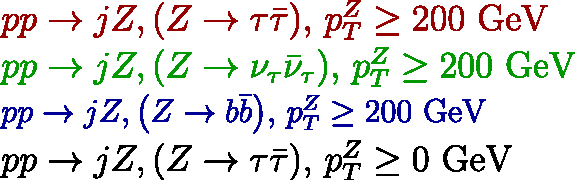
\includegraphics[width=0.5\textwidth]{./ColorConventions.pdf}
\end{center}
We present some simple results obtained using jet substructure variables on jets tagged using BDRS+Filtering methods (Note: we use the final 2 step filtered (BDRS\cite{BDRS}+filtering) jet to evaluate variables and all of these results are for events with MPI enabled). Note that planar flow \cite{PlanarFlow} [\autoref{fig:PlanarFlow}, \autoref{fig:PlanarFlowX}] seem to work extremely well.


\begin{figure}[H]
    \begin{center}
        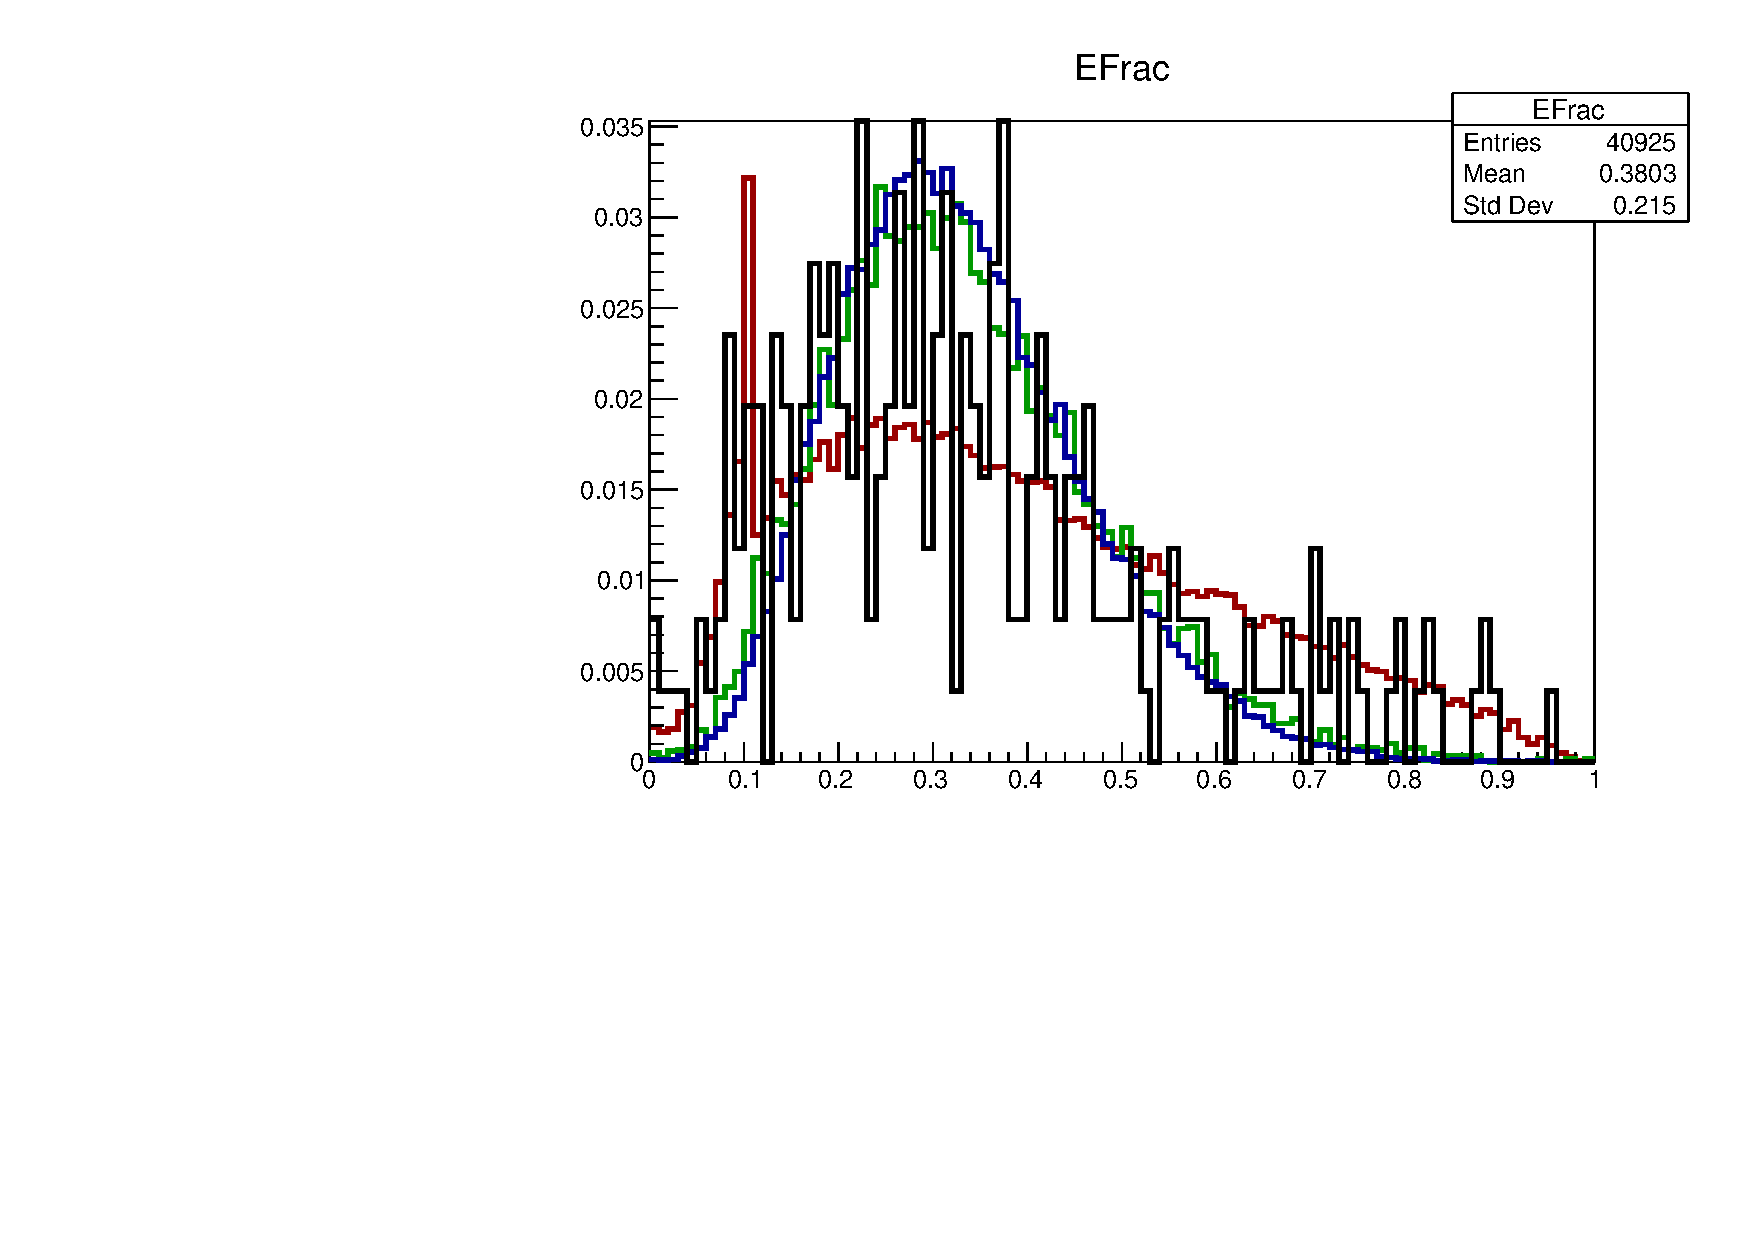
\includegraphics[width=0.7\textwidth]{./EFrac.pdf}
        \caption{ Electromagnetic energy fraction of the jet, normalized to unit area under the curve. }
        \label{fig:EFrac}
    \end{center}
\end{figure}

\begin{figure}[H]
    \begin{center}
        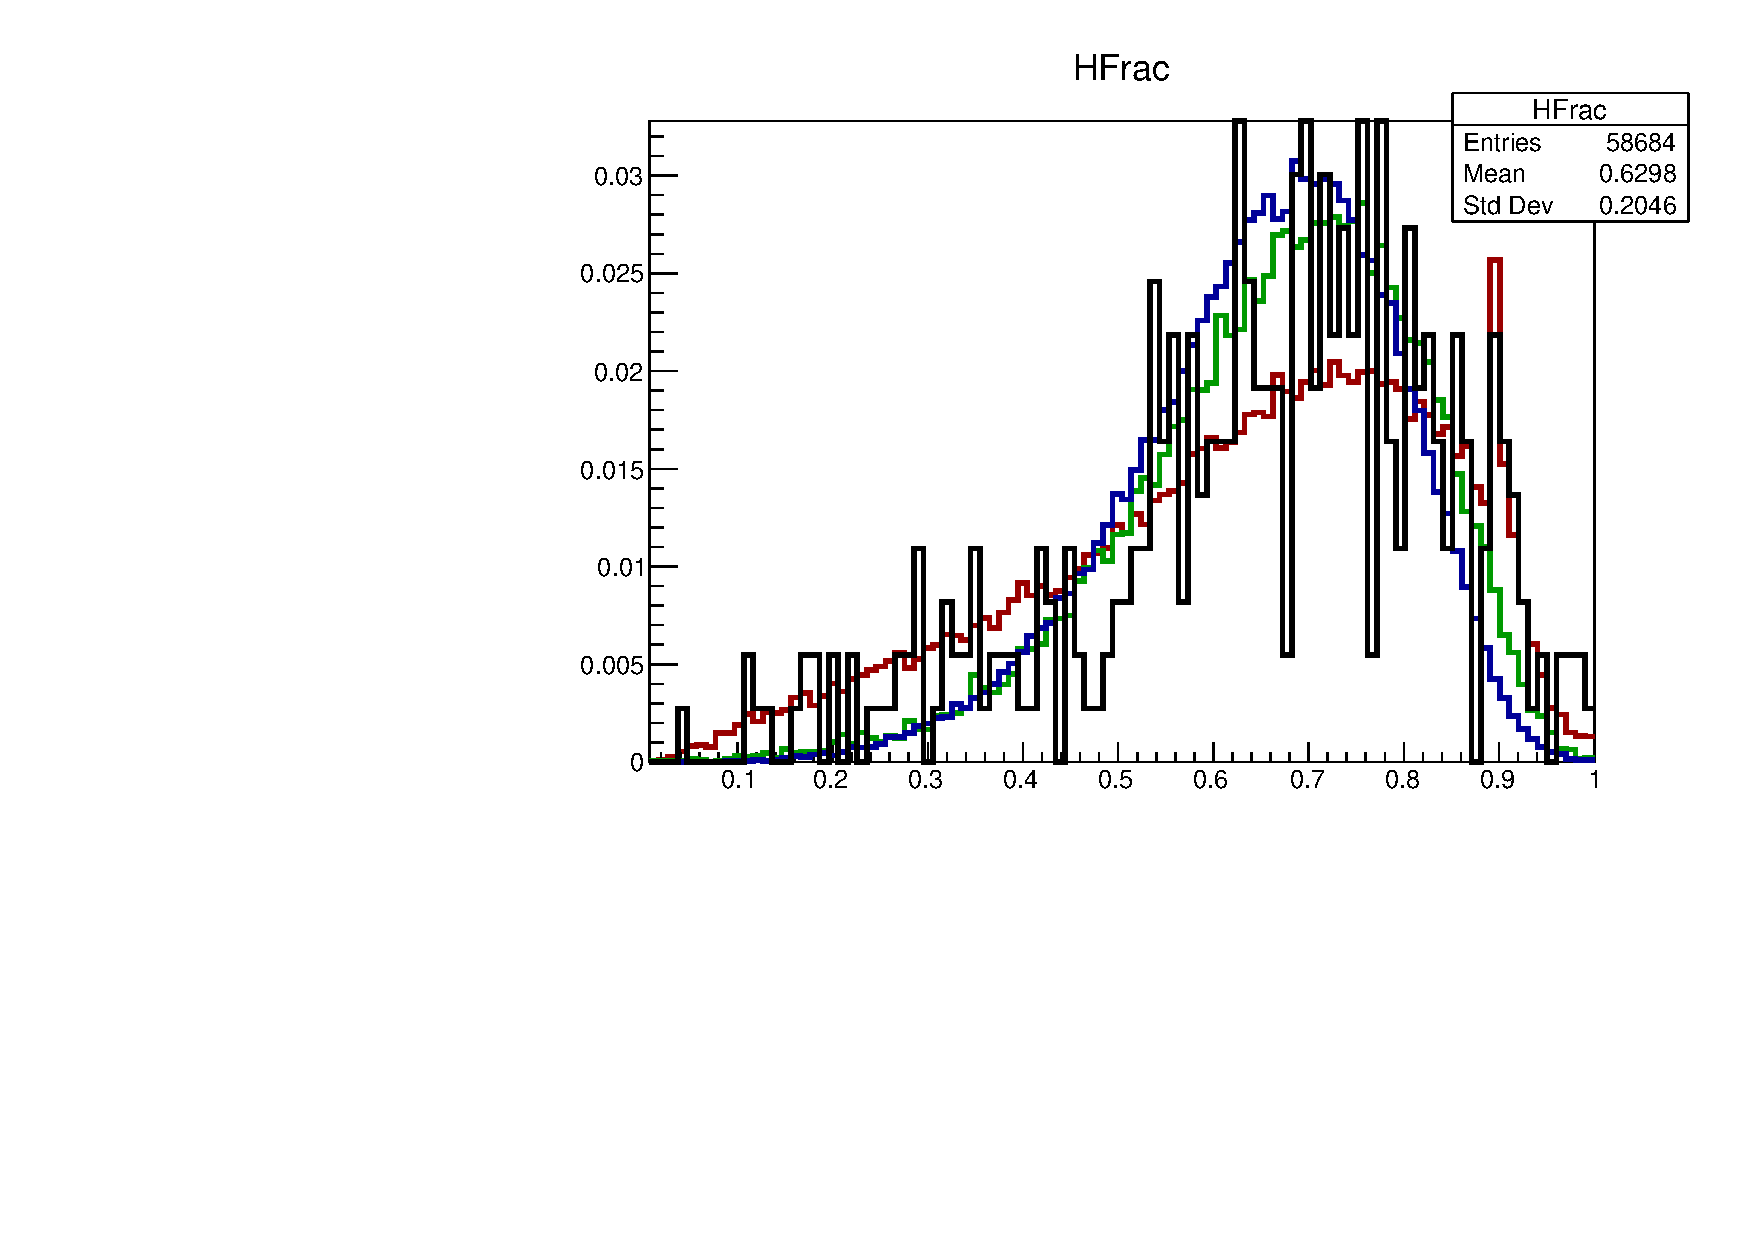
\includegraphics[width=0.7\textwidth]{./HFrac.pdf}
        \caption{ Hadronic energy fraction of the jet, normalized to unit area under the curve. }
        \label{fig:HFrac}
    \end{center}
\end{figure}

\begin{figure}[H]
    \begin{center}
        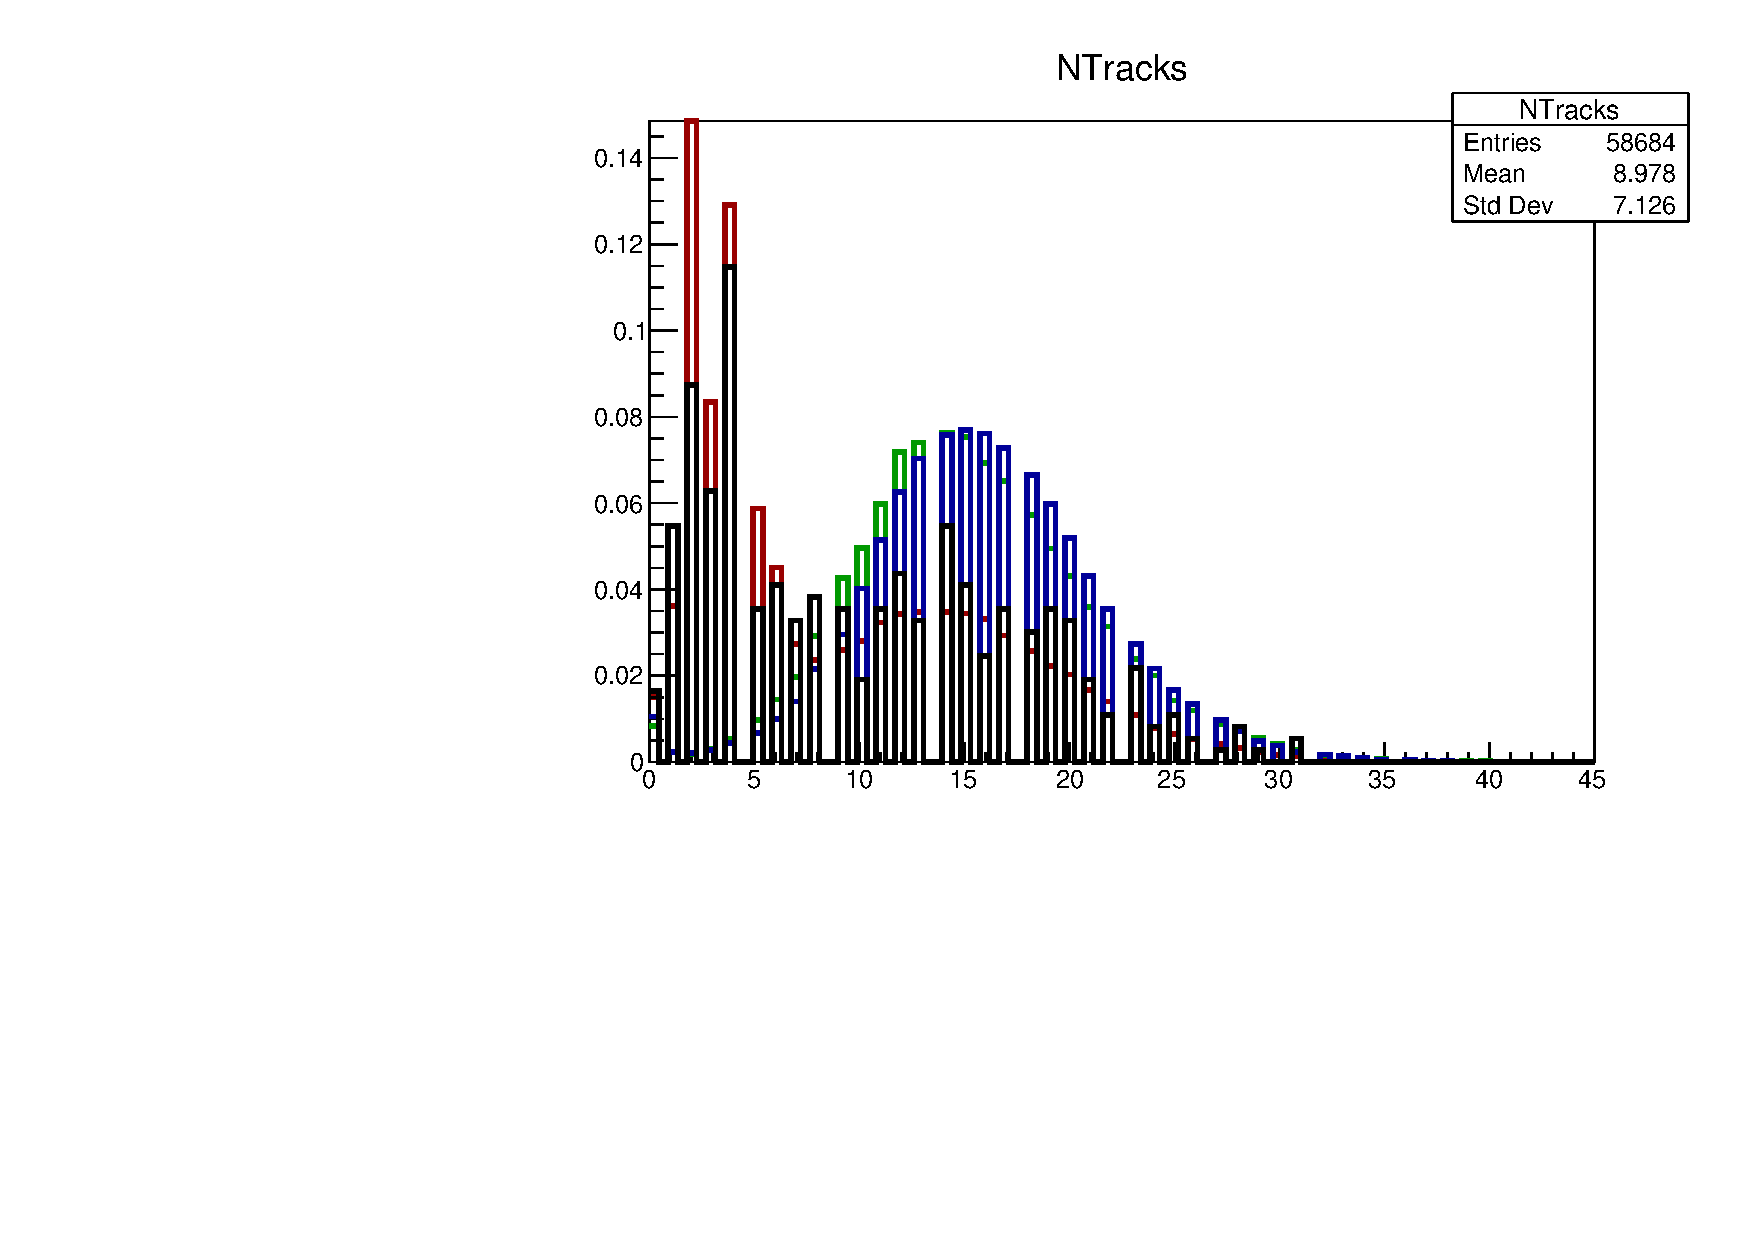
\includegraphics[width=0.7\textwidth]{./NTracks.pdf}
        \caption{ Number of tracks in the jet, normalized to unit area under the curve. }
        \label{fig:NTracks}
    \end{center}
\end{figure}

\begin{figure}[H]
    \begin{center}
        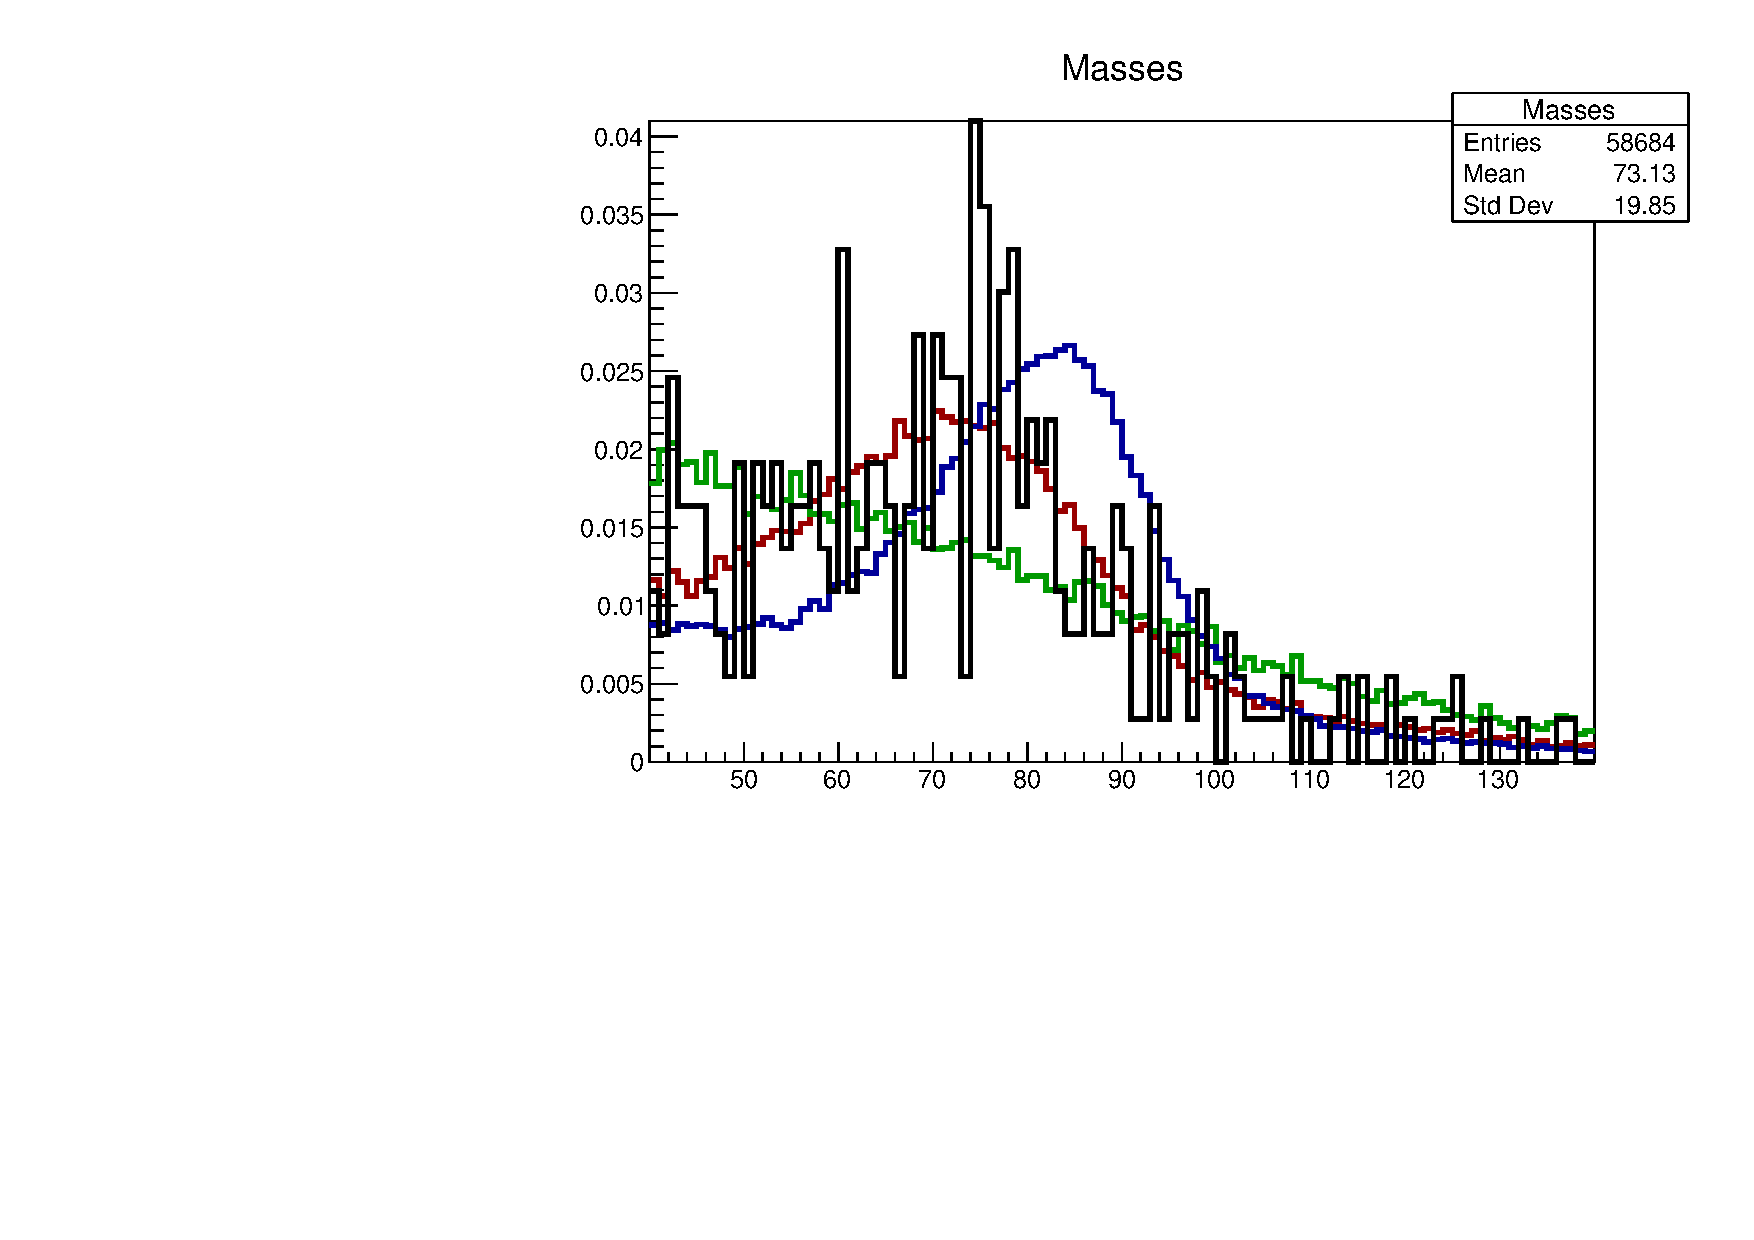
\includegraphics[width=0.7\textwidth]{./Masses.pdf}
        \caption{ Masses of the jet after BDRS and filtering steps, normalized to unit area under the curve. }
        \label{fig:Masses}
    \end{center}
\end{figure}

\begin{figure}[H]
    \begin{center}
        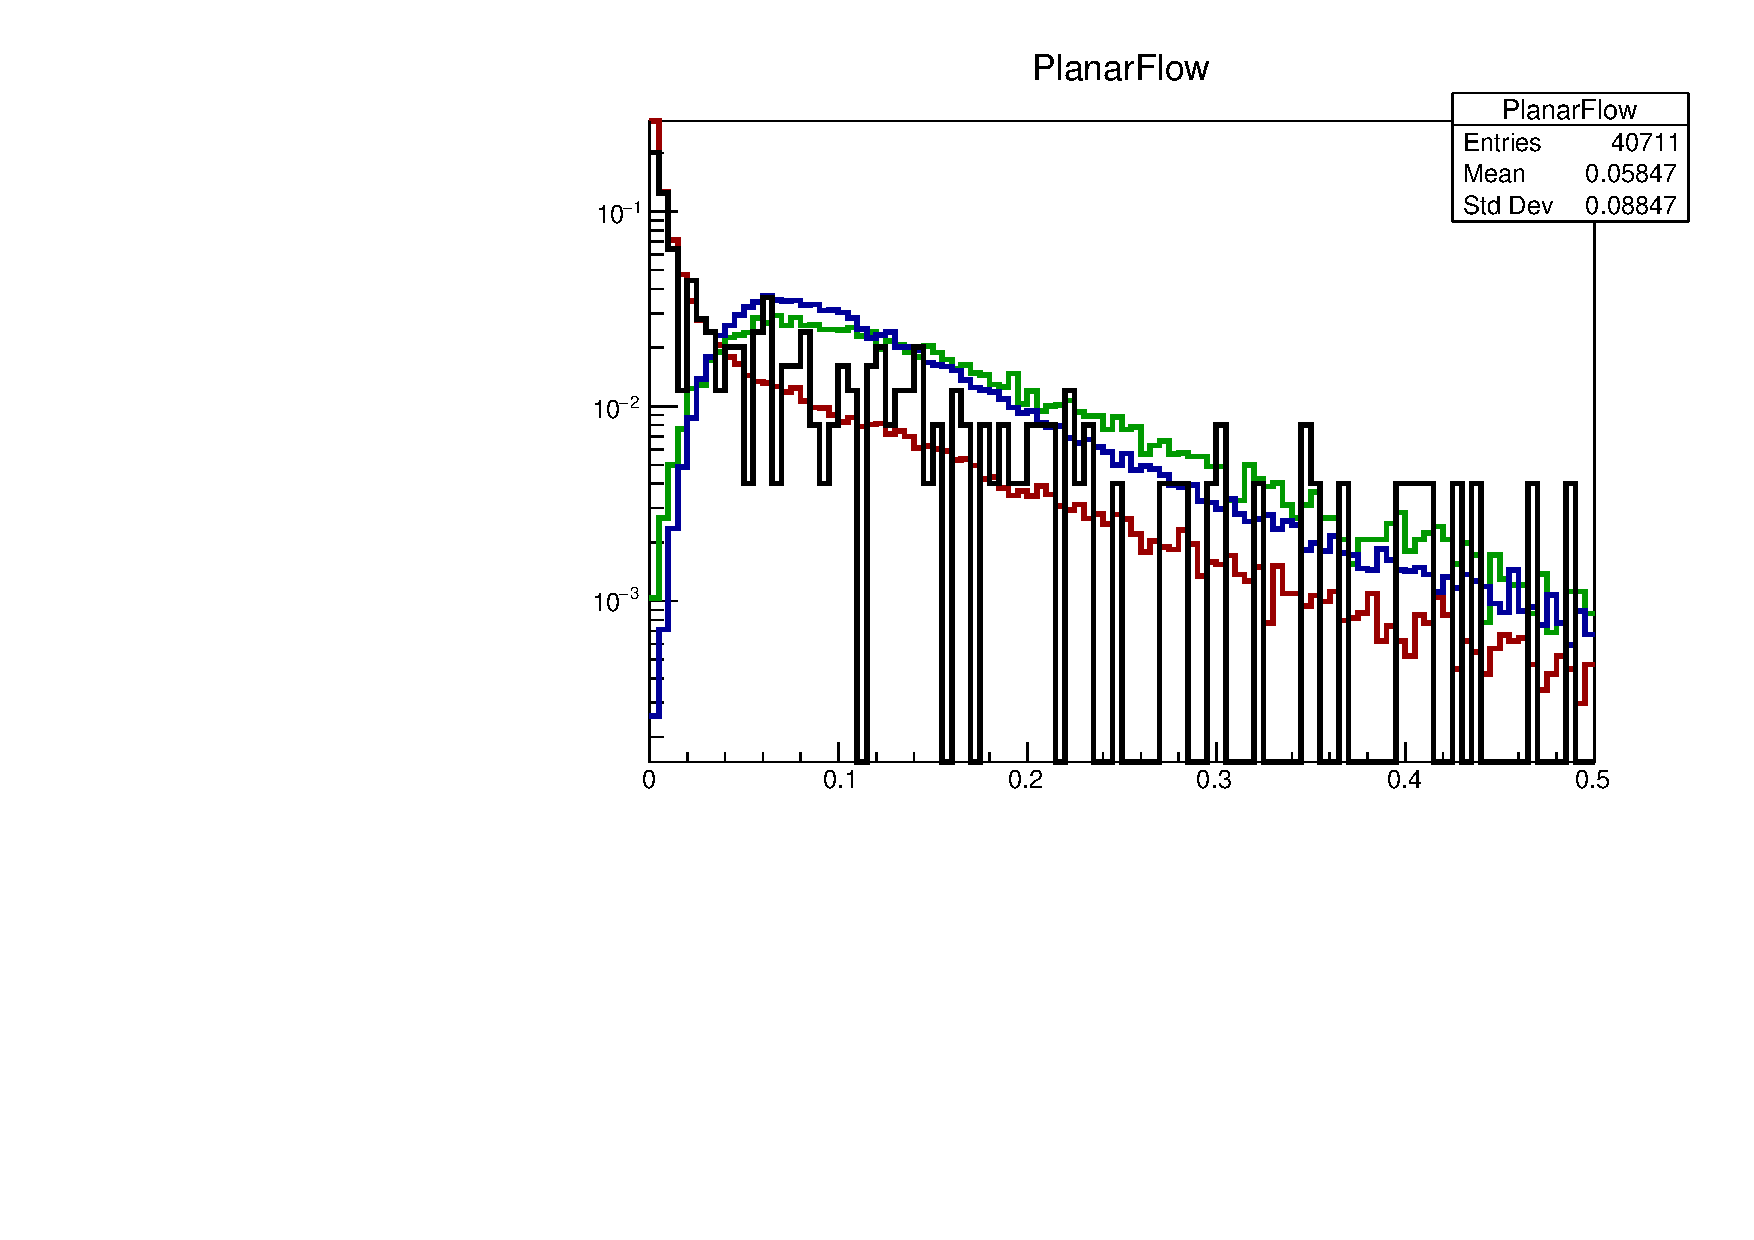
\includegraphics[width=0.7\textwidth]{./PlanarFlow.pdf}
        \caption{ Planar Flow of the jet after BDRS and filtering steps, normalized to unit area under the curve. }
        \label{fig:PlanarFlow}
    \end{center}
\end{figure}

\begin{figure}[H]
    \begin{center}
        
\includegraphics[width=0.49\textwidth]{./PlanarFlow1.pdf}
        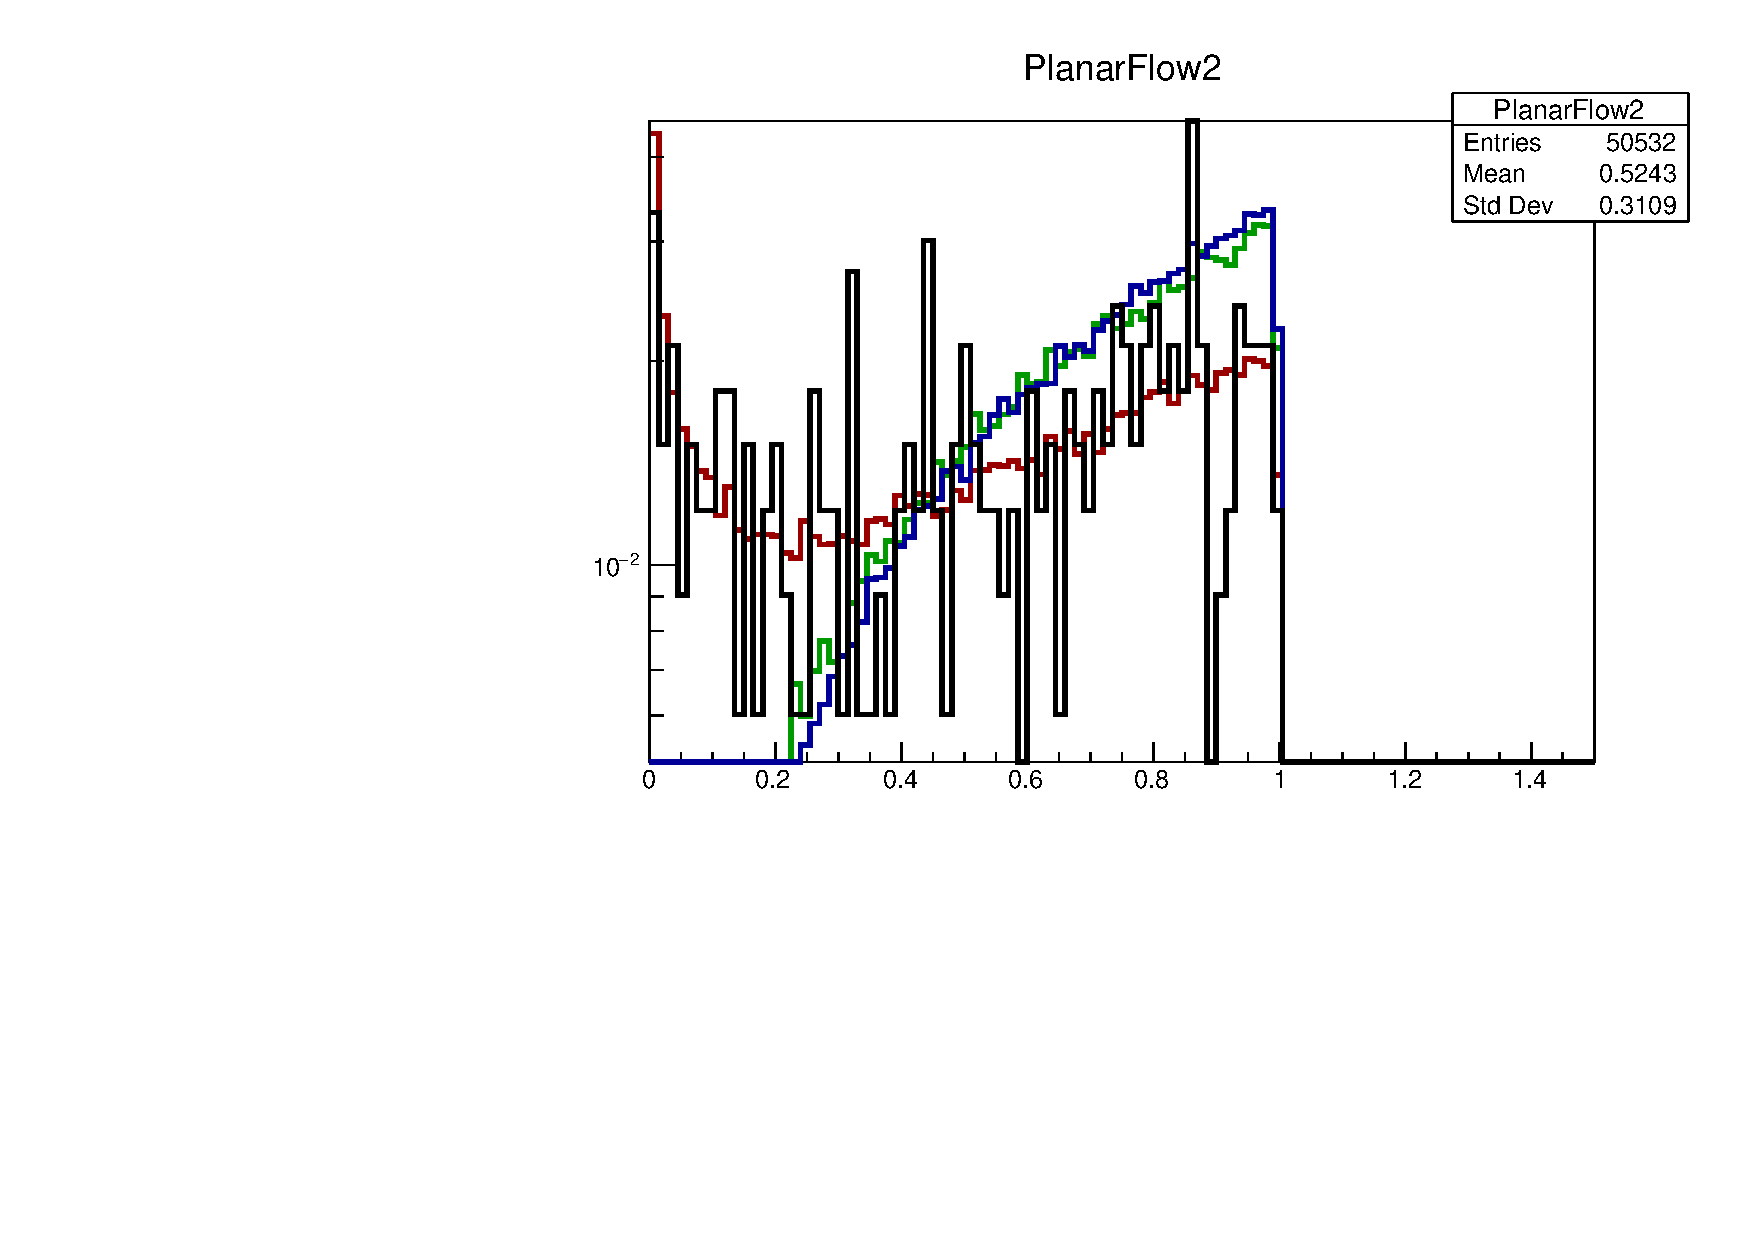
\includegraphics[width=0.49\textwidth]{./PlanarFlow2.pdf}\\
        \caption{ Planar Flow of the two subjets after BDRS and filtering steps, normalized to unit area under the curve. }
        \label{fig:PlanarFlowX}
    \end{center}
\end{figure}

\begin{figure}[H]
    \begin{center}
        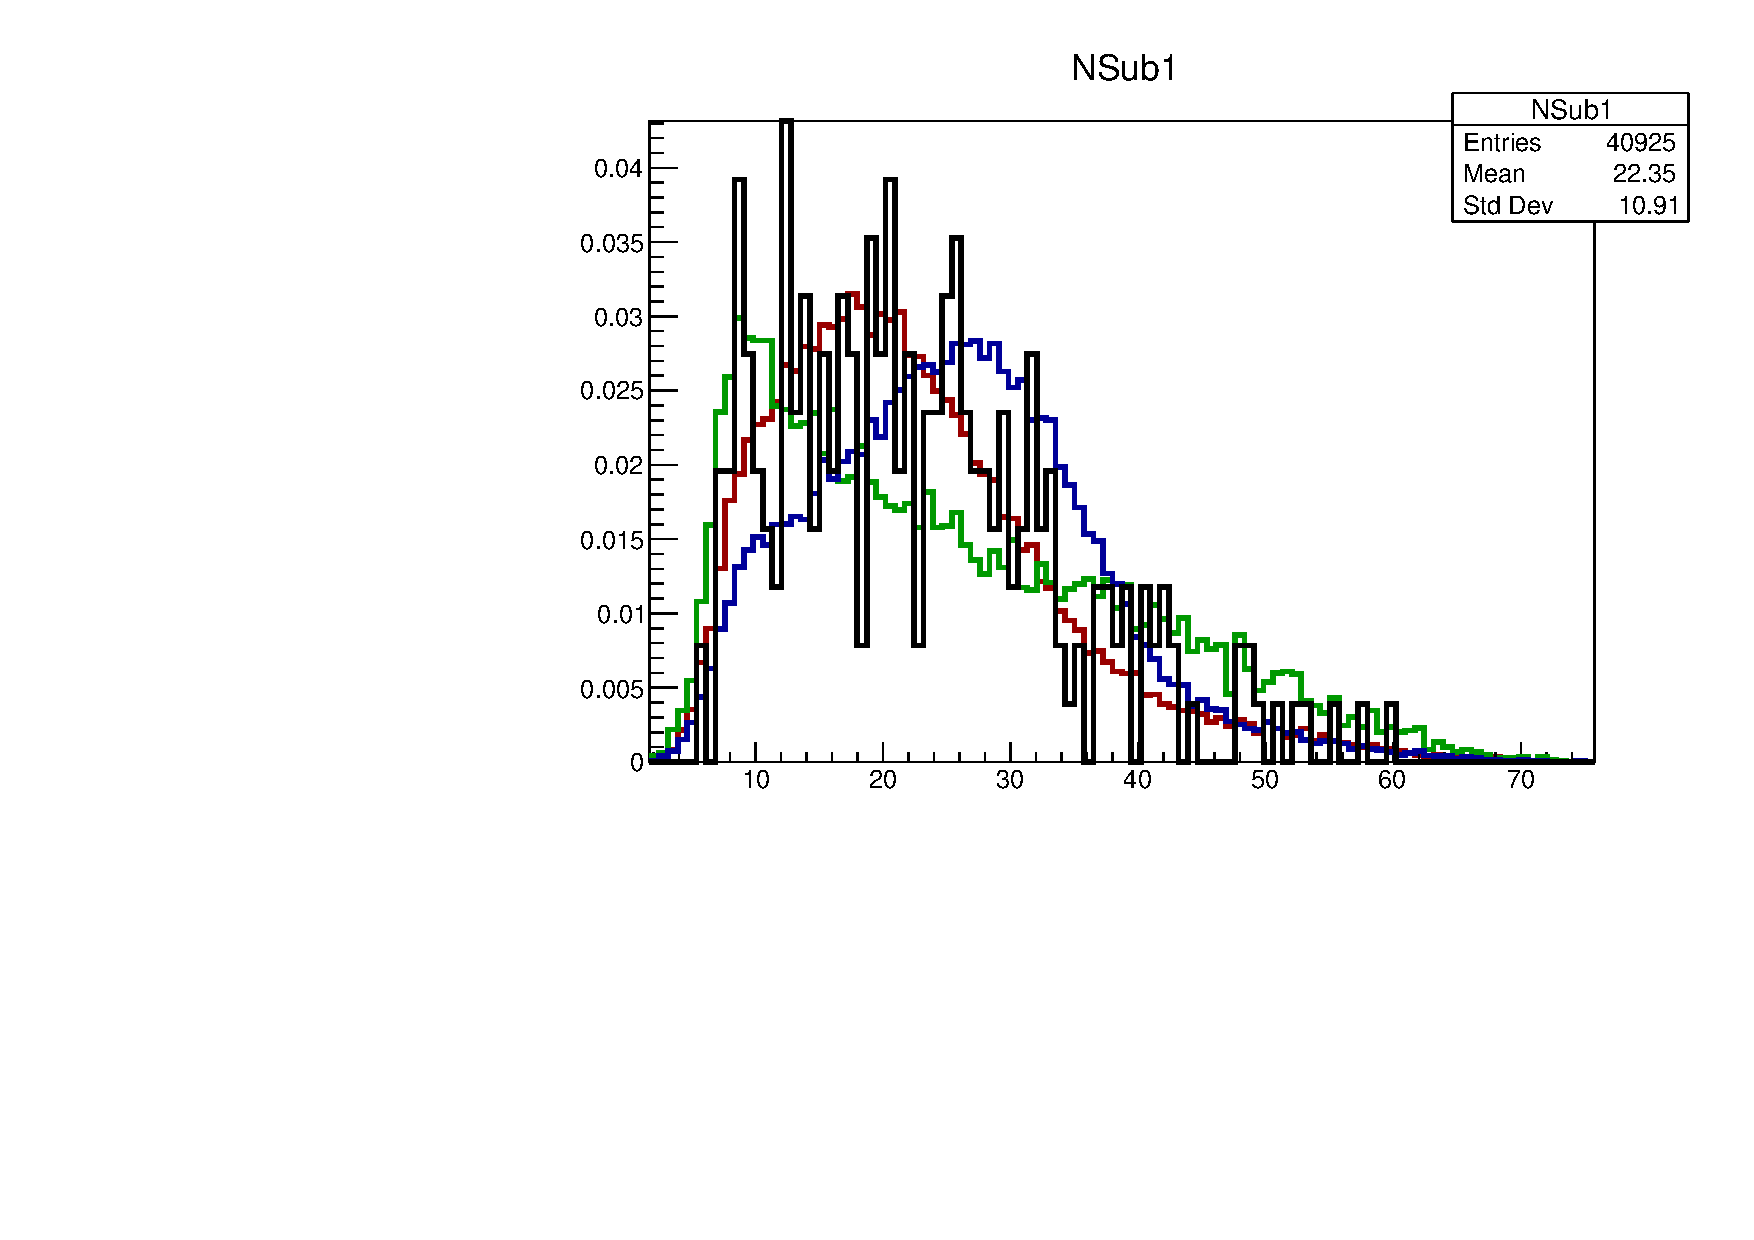
\includegraphics[width=0.49\textwidth]{./NSub1.pdf}
        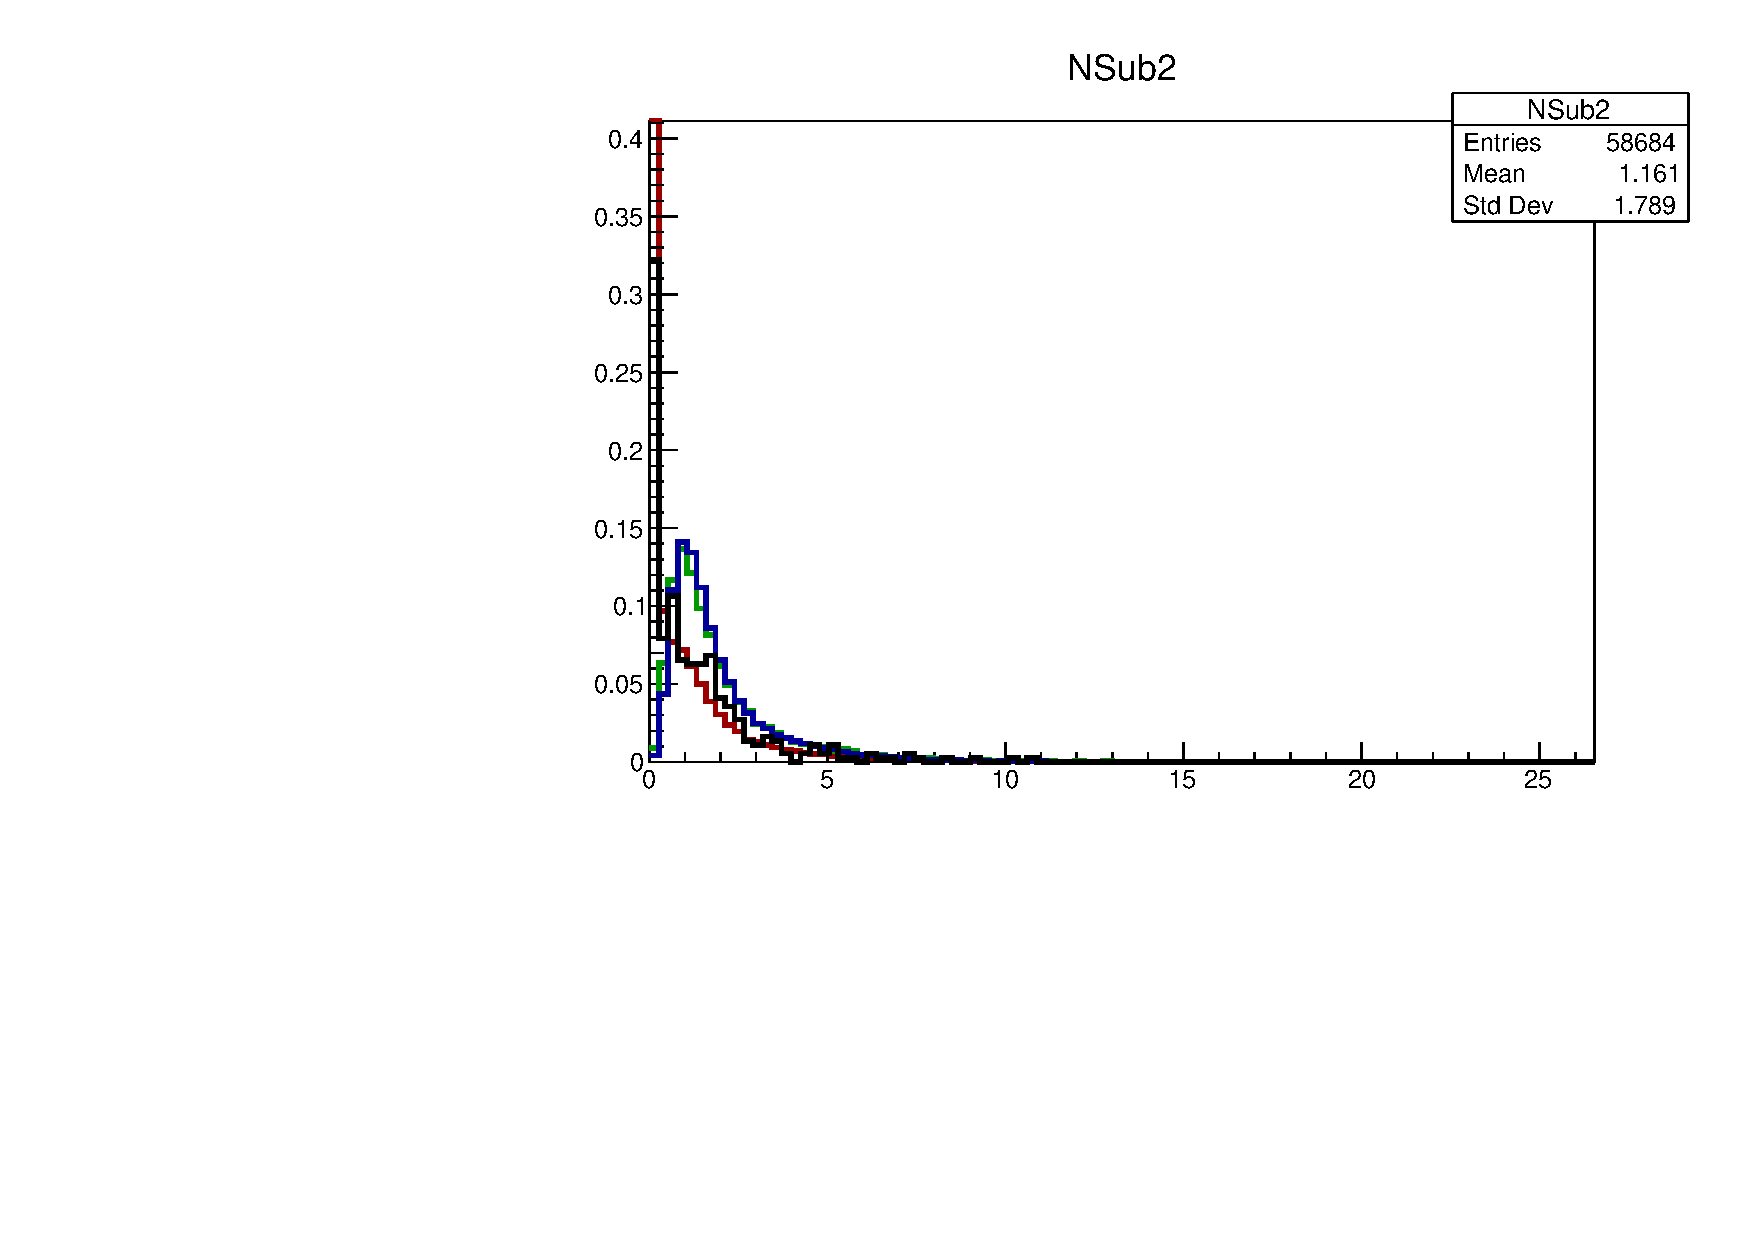
\includegraphics[width=0.49\textwidth]{./NSub2.pdf}\\
        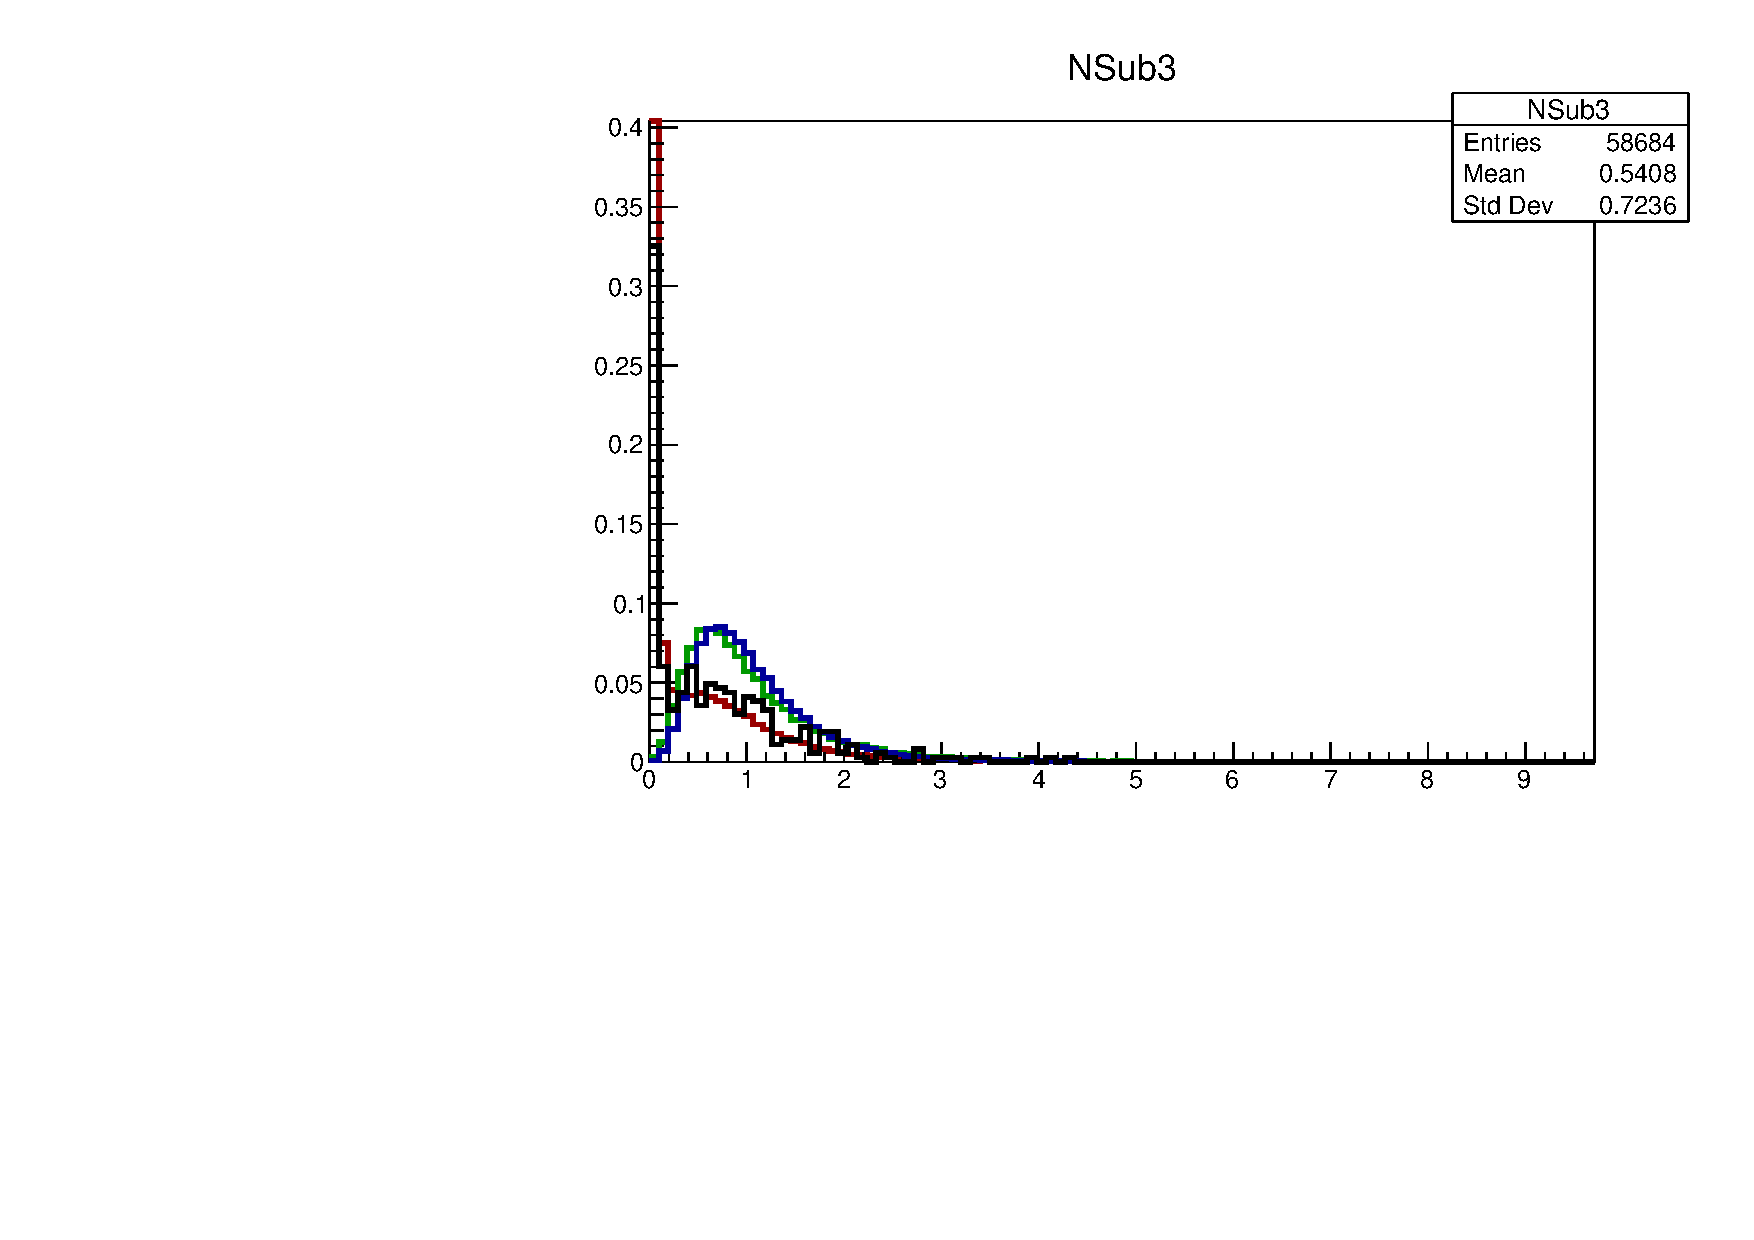
\includegraphics[width=0.49\textwidth]{./NSub3.pdf}
        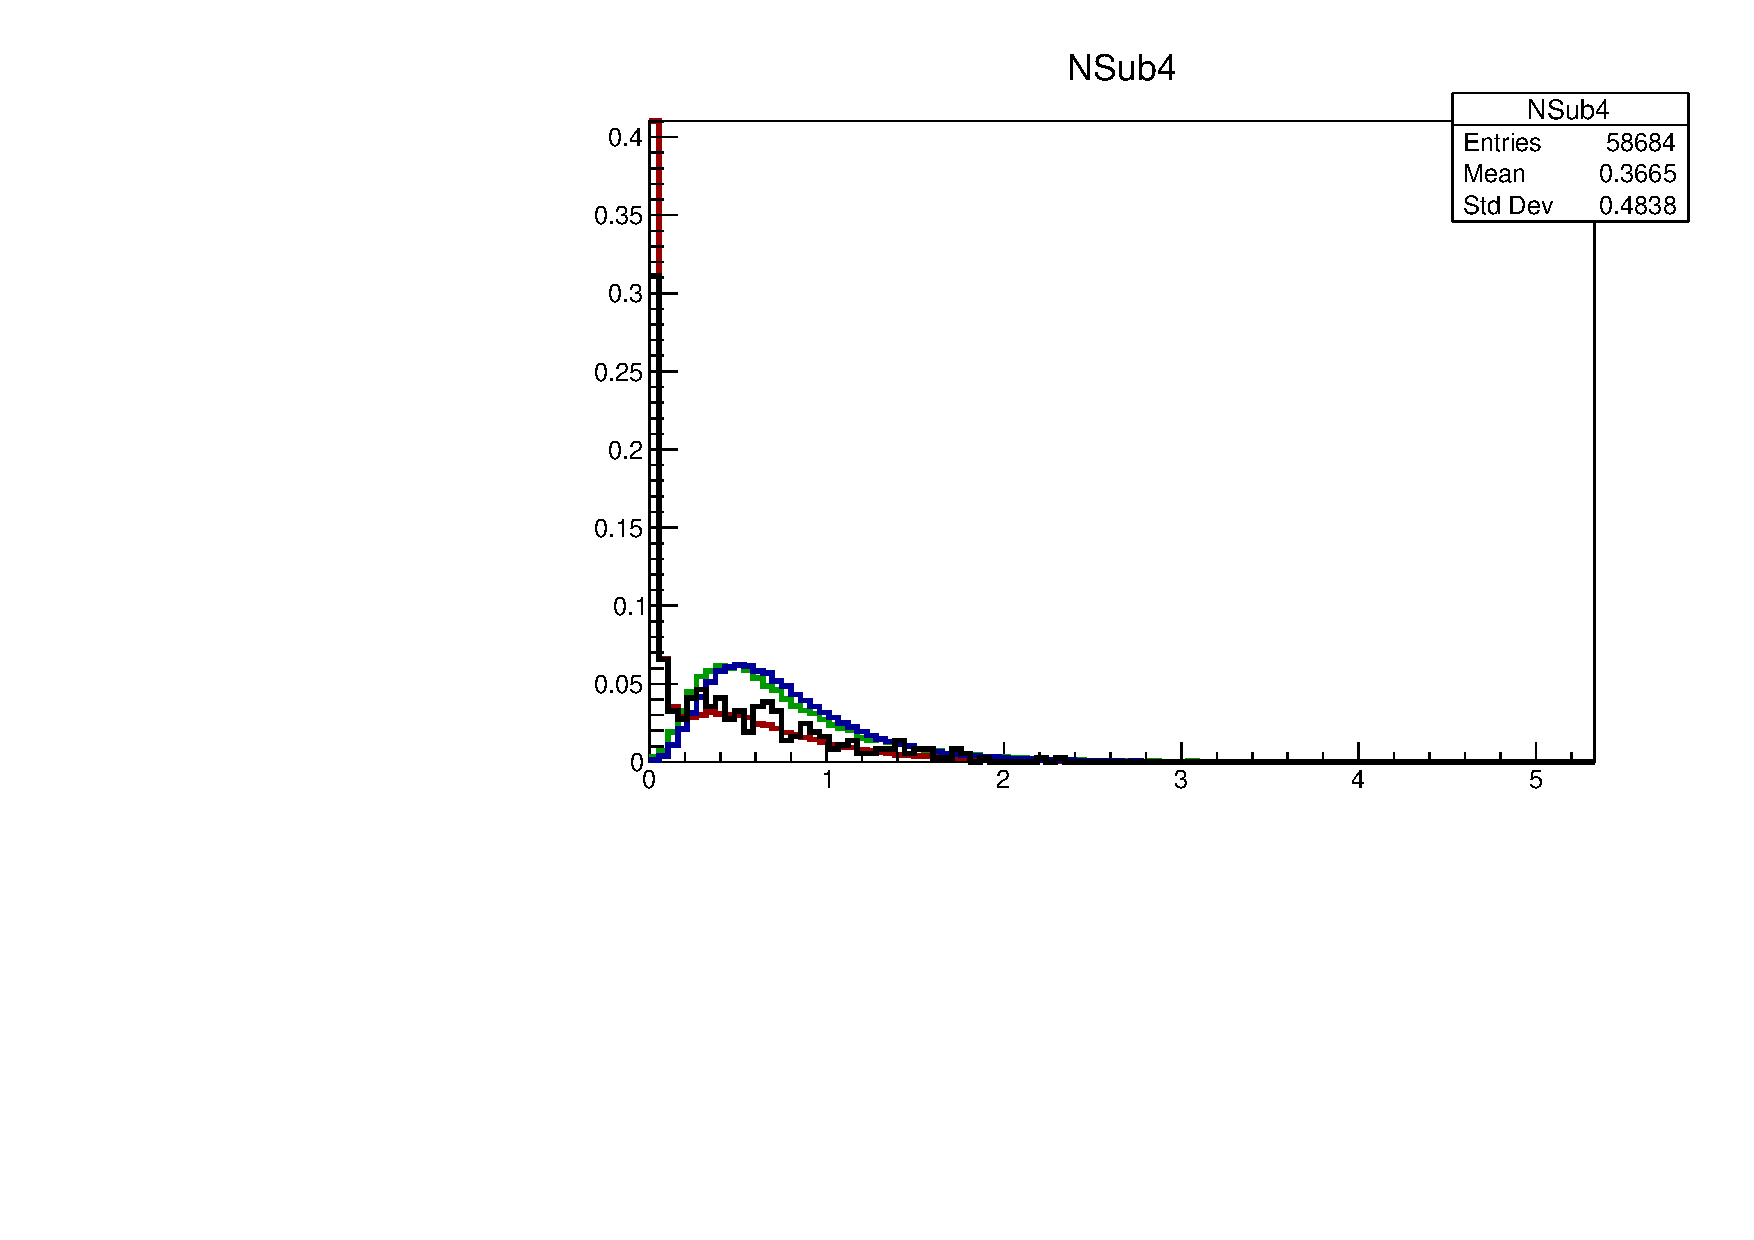
\includegraphics[width=0.49\textwidth]{./NSub4.pdf}\\
        \caption{ {\tt NSubJettiness} observable, normalized to unit area under the curve. }
        \label{fig:NSub}
    \end{center}
\end{figure}

\begin{figure}[H]
    \begin{center}
        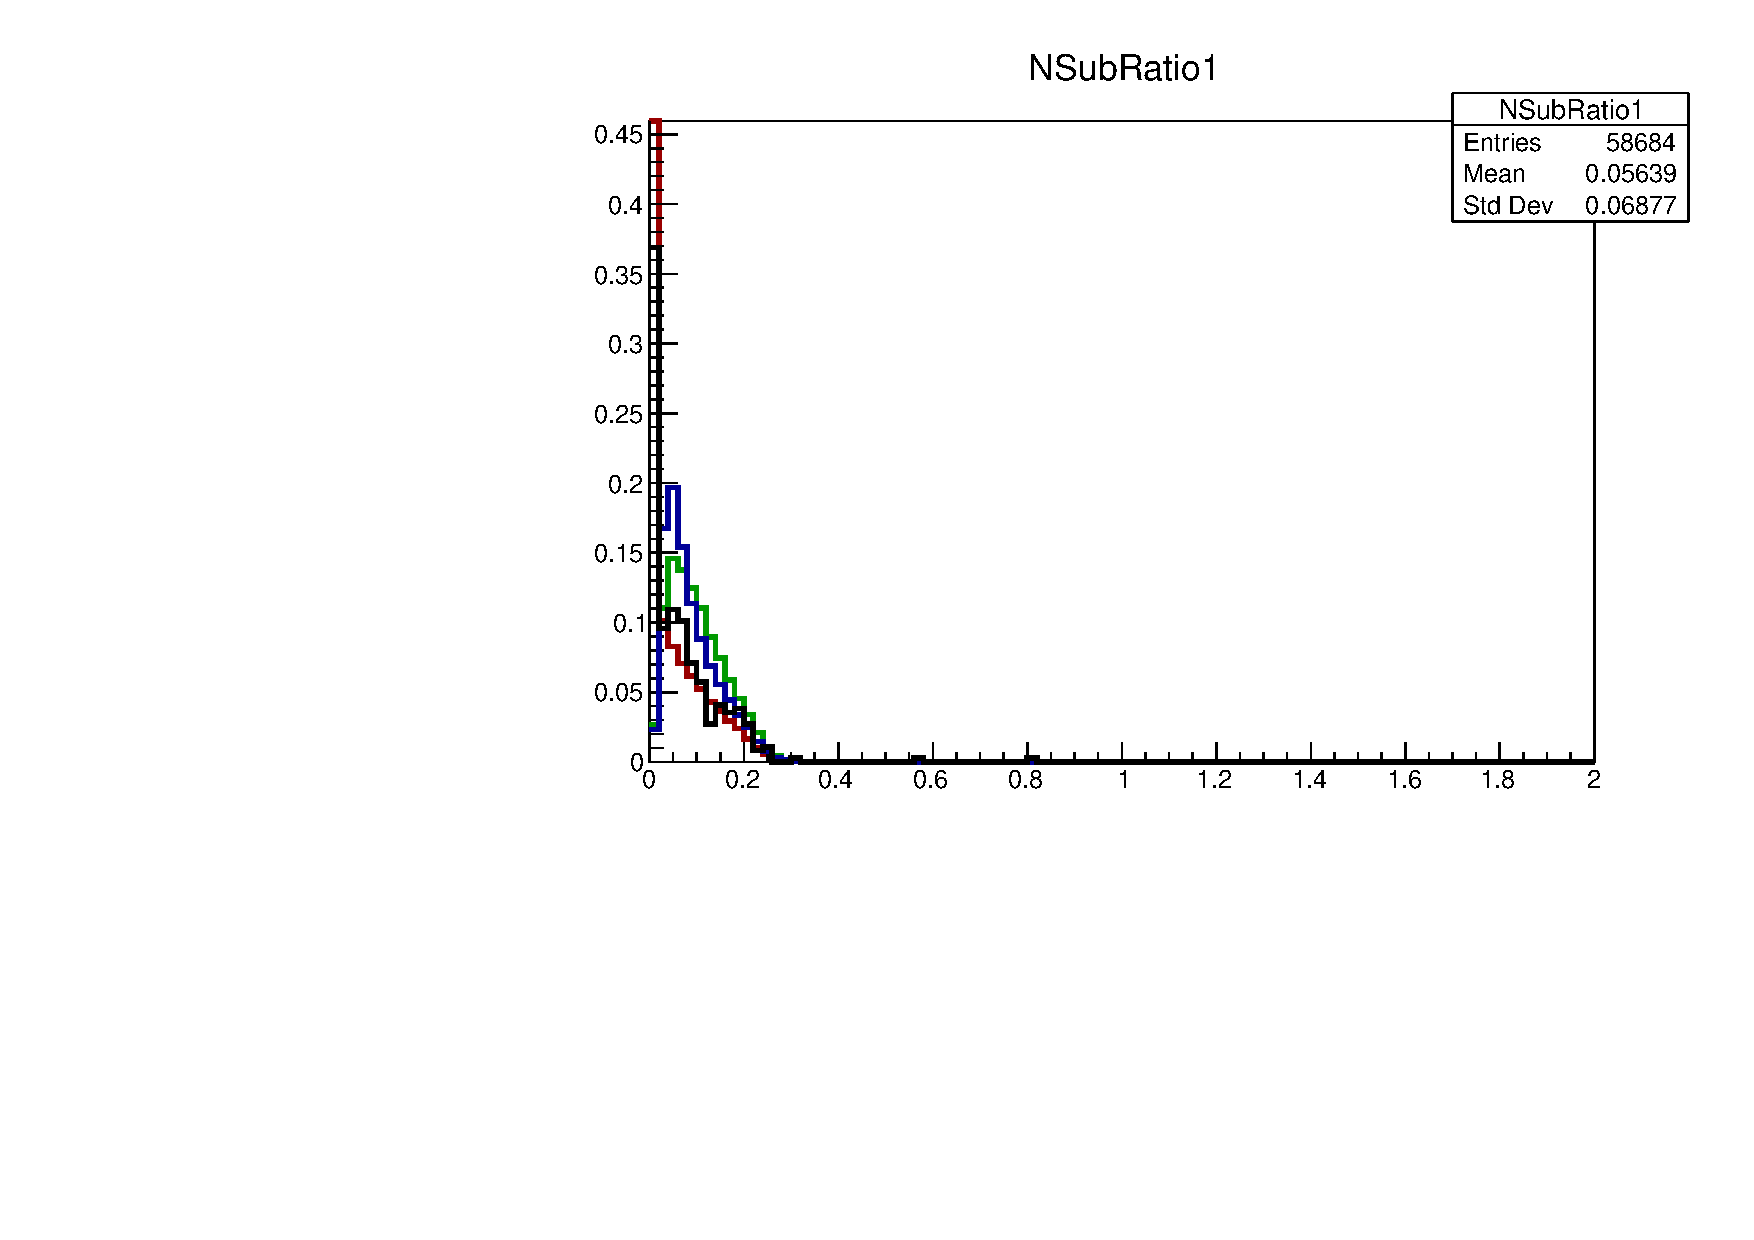
\includegraphics[width=0.49\textwidth]{./NSubRatio1.pdf}
        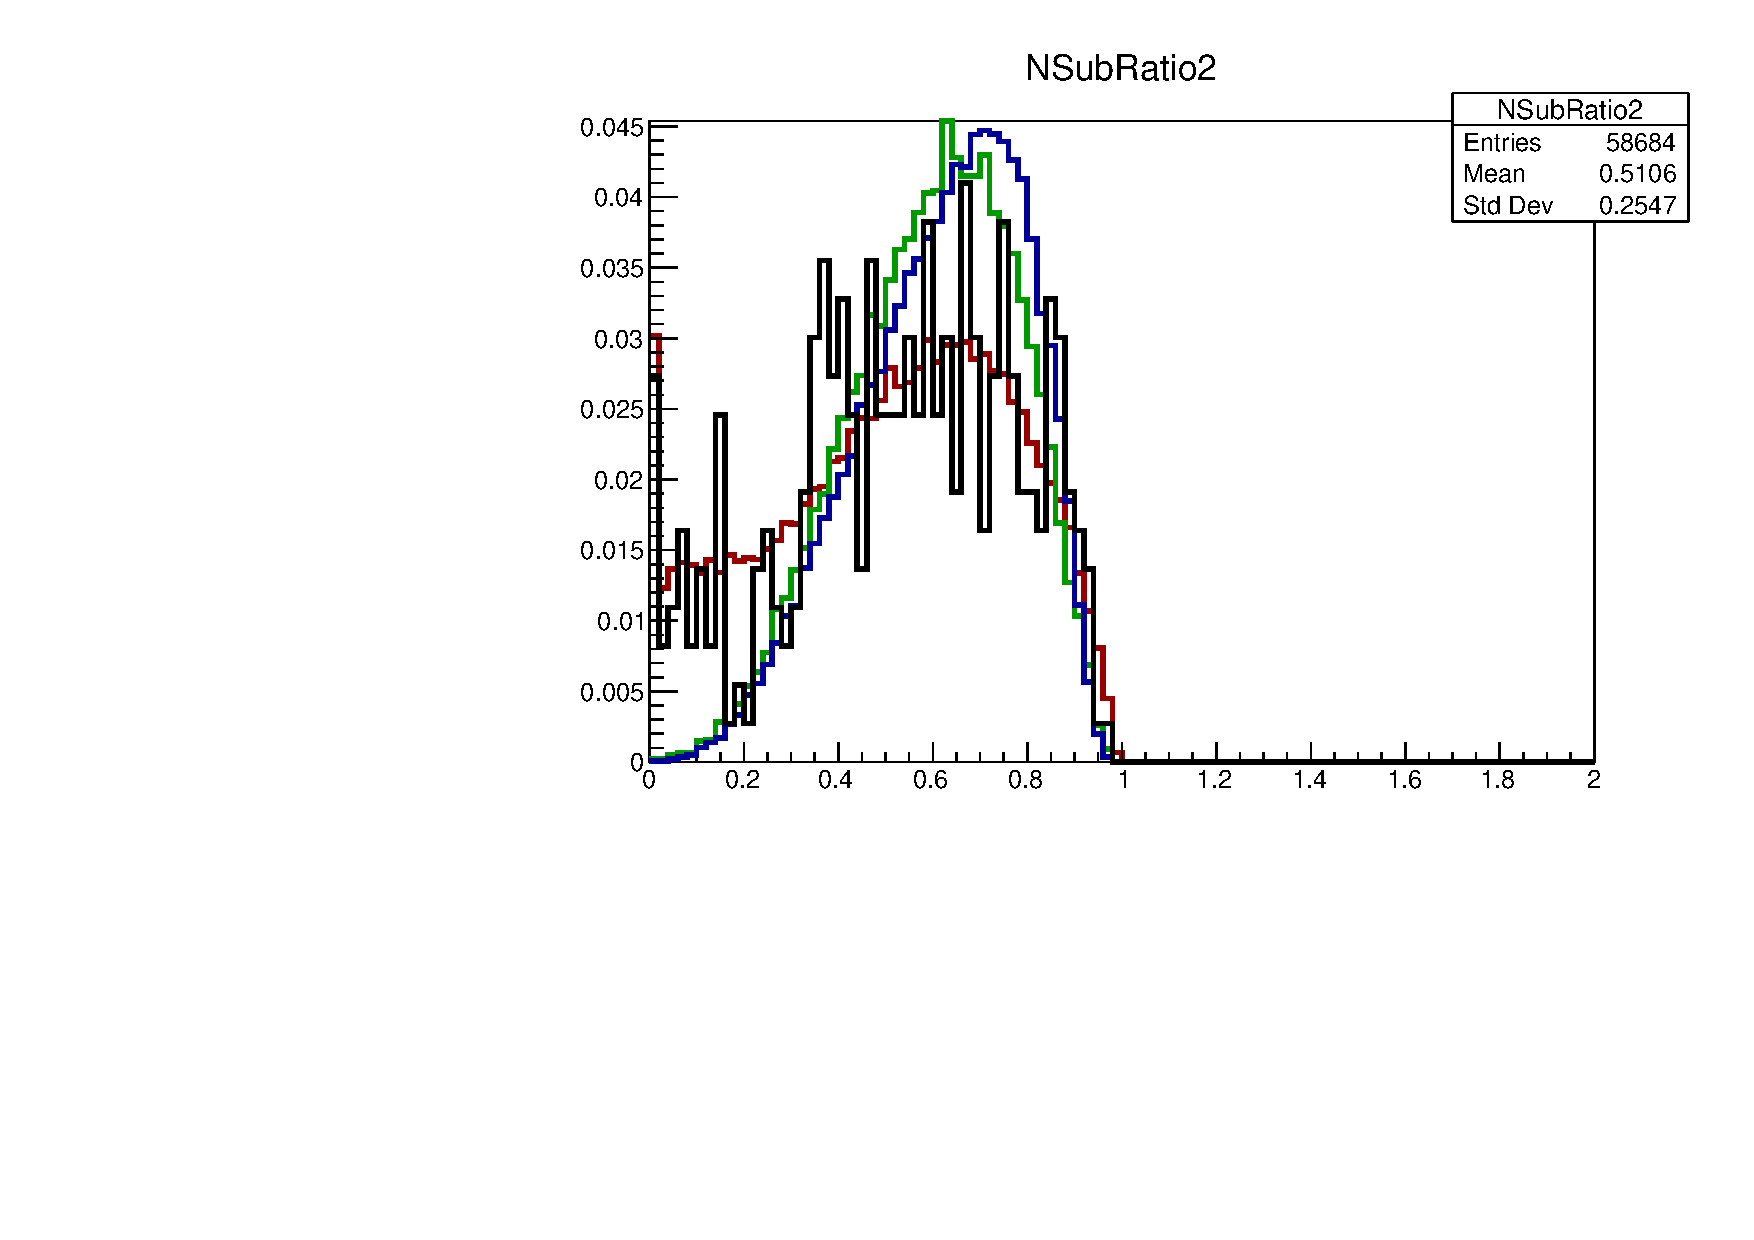
\includegraphics[width=0.49\textwidth]{./NSubRatio2.pdf}\\
        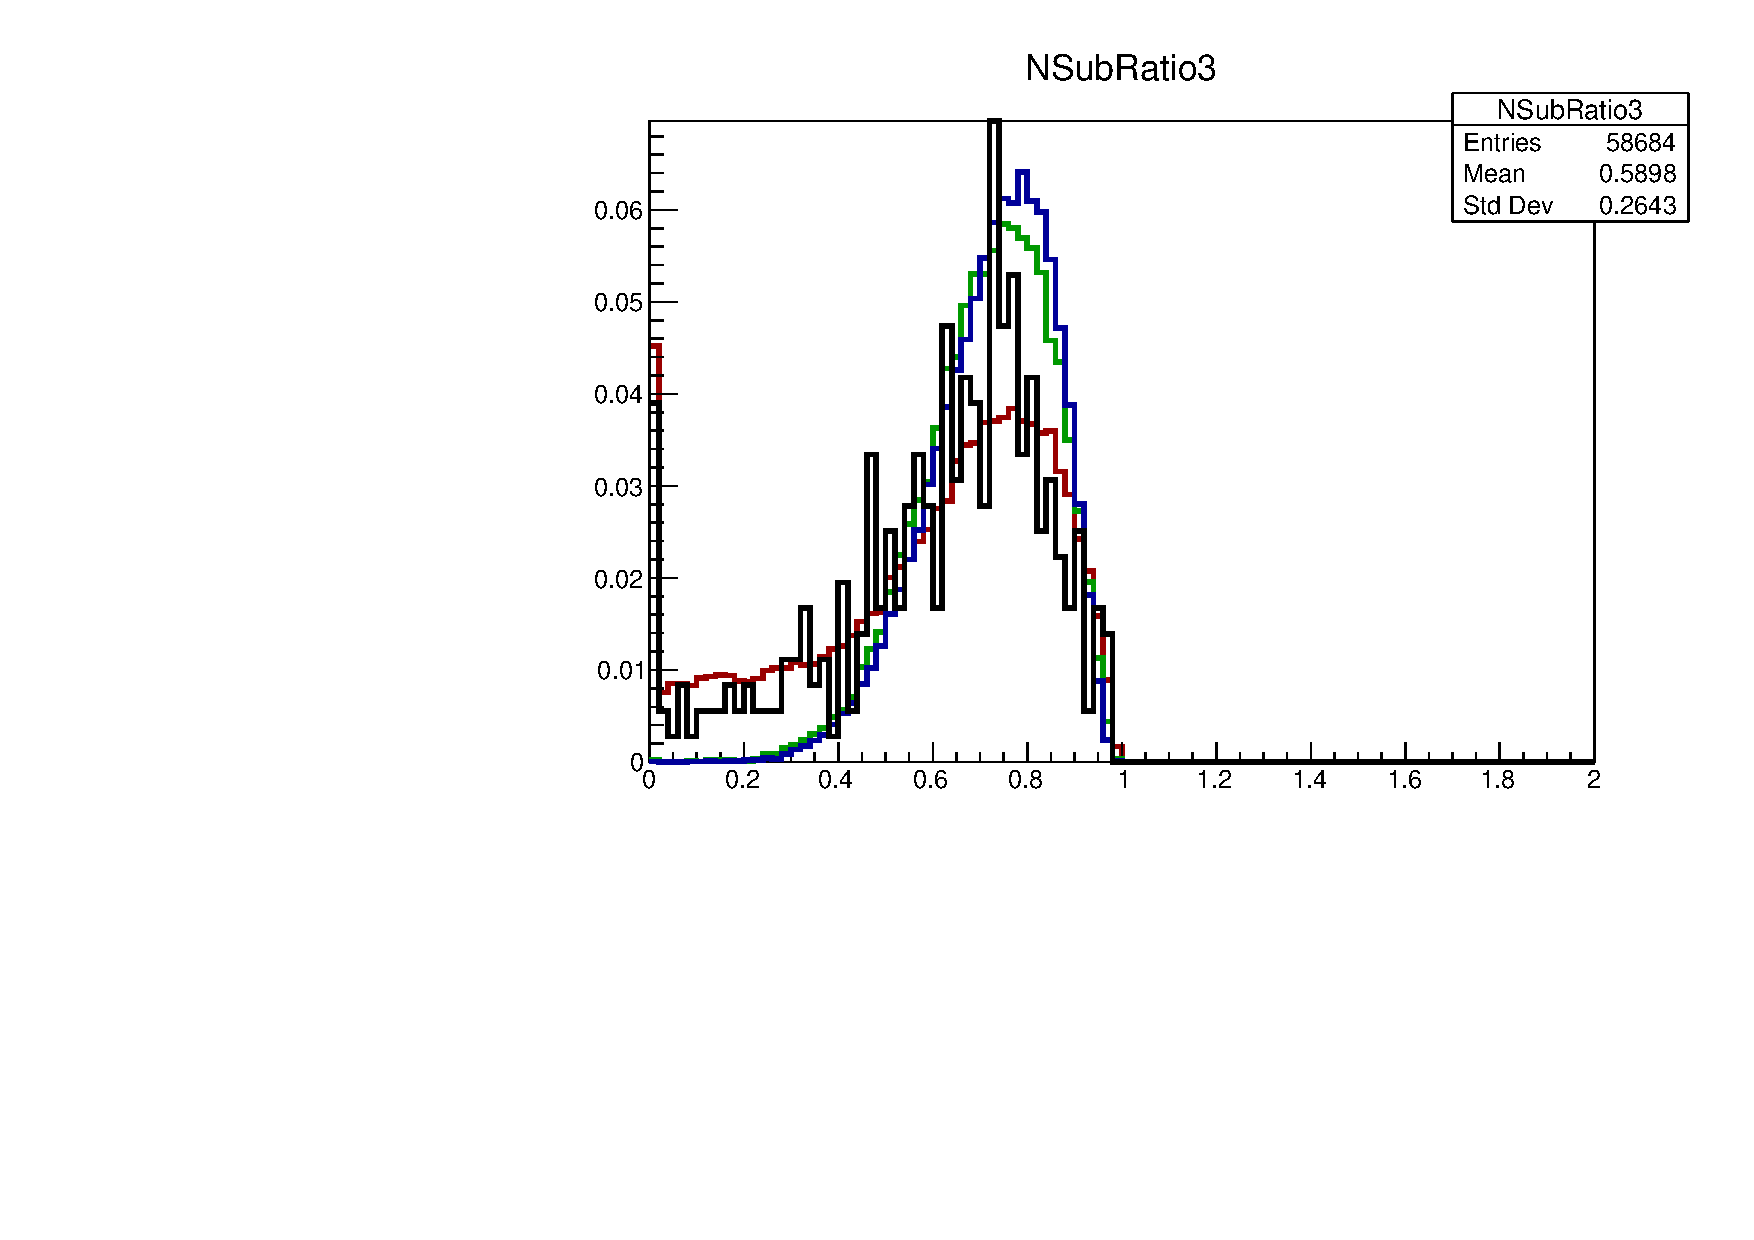
\includegraphics[width=0.49\textwidth]{./NSubRatio3.pdf}
        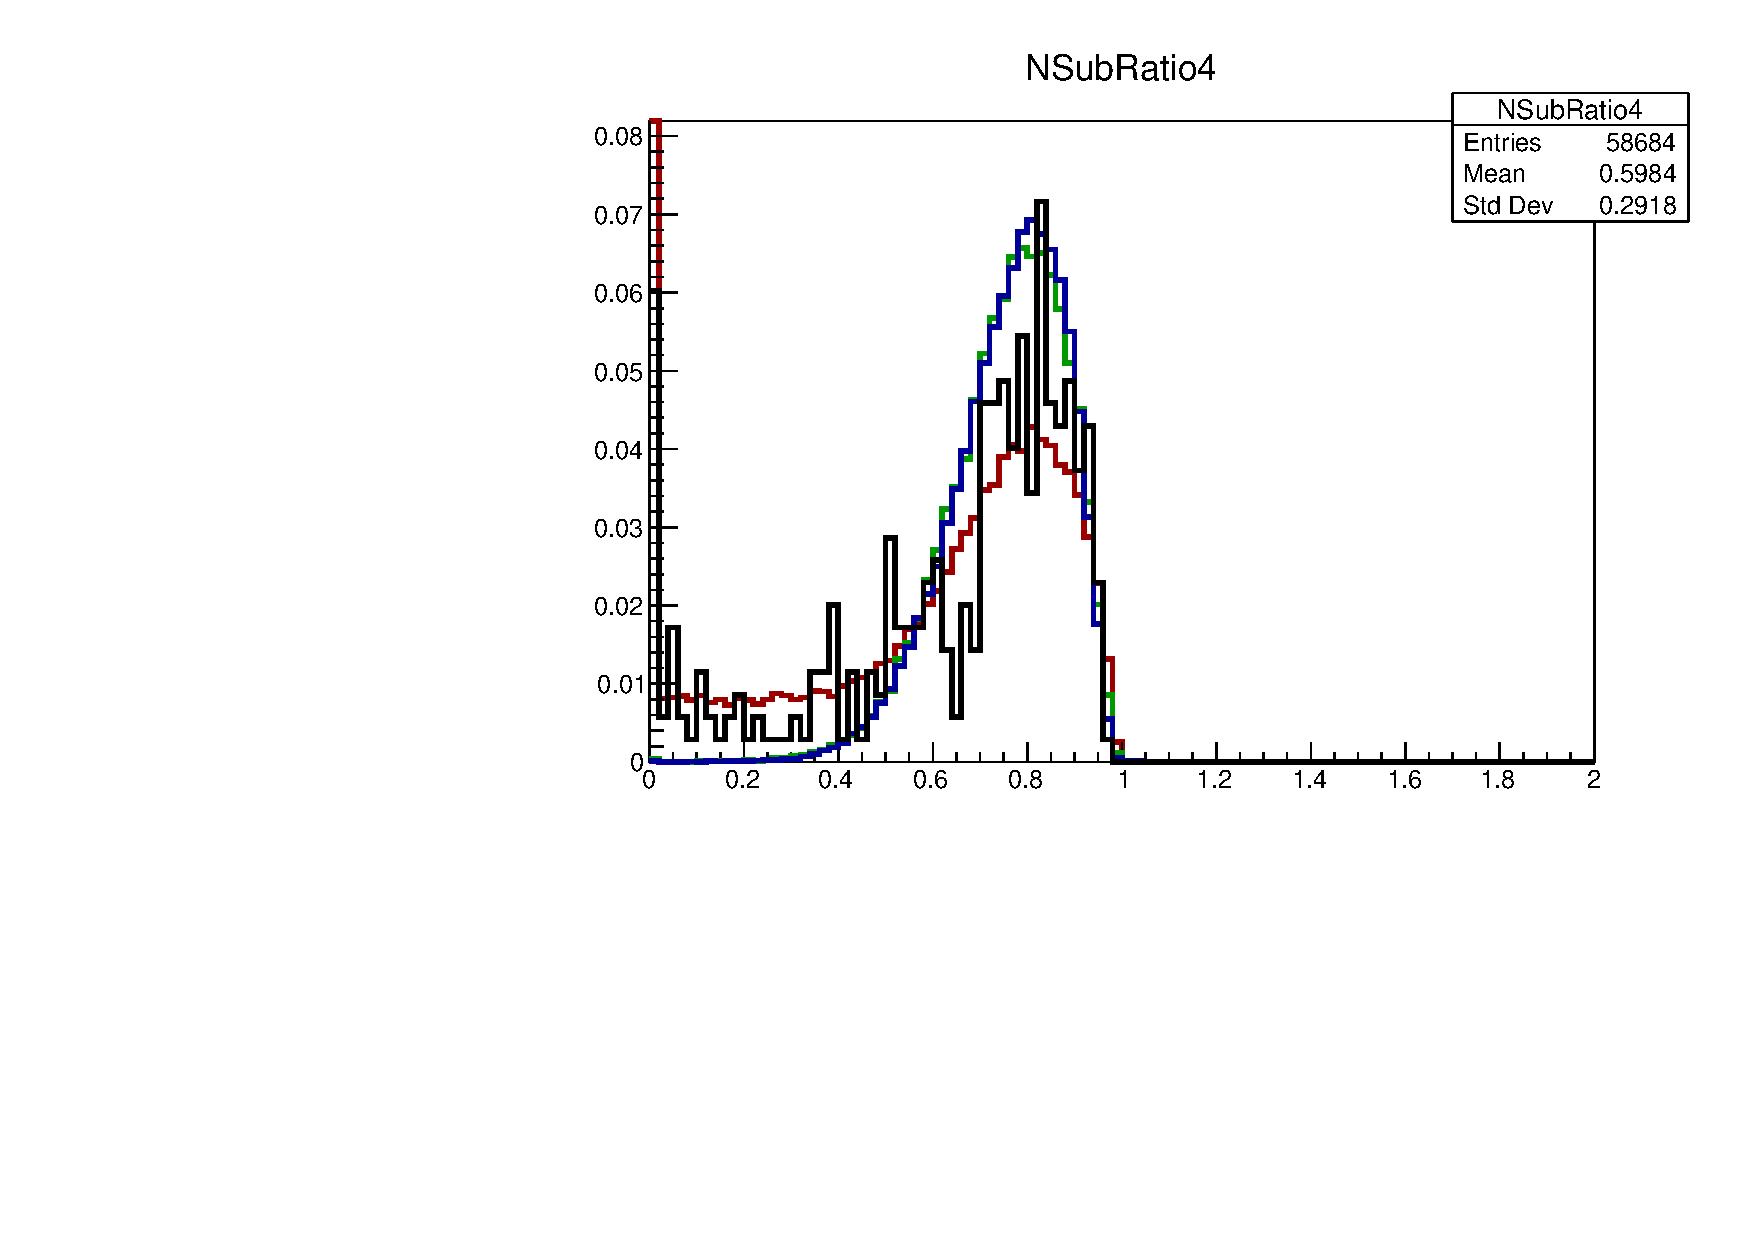
\includegraphics[width=0.49\textwidth]{./NSubRatio4.pdf}\\
        \caption{ Ratio of {\tt NSubJettiness} observable, normalized to unit area under the curve. }
        \label{fig:NSubRatio}
    \end{center}
\end{figure}

\begin{figure}[H]
    \begin{center}
        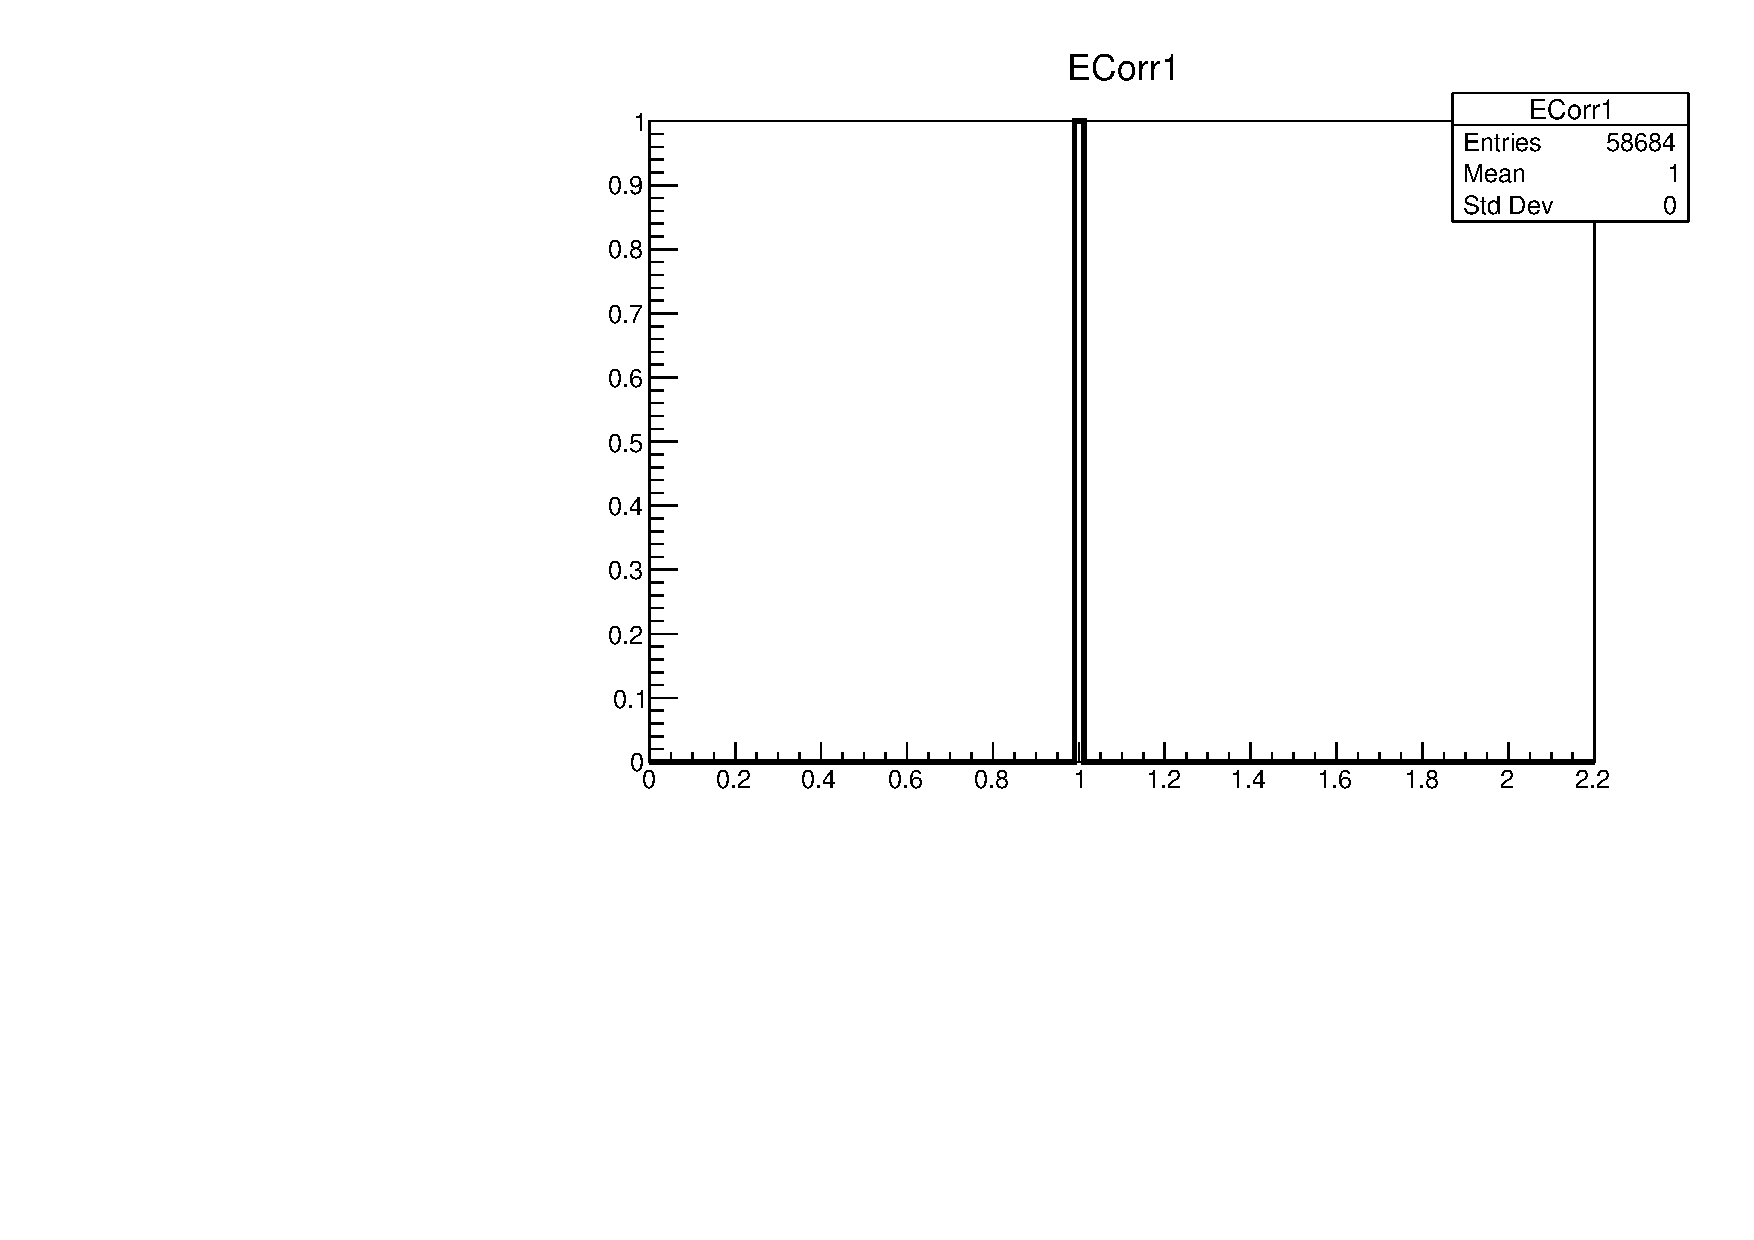
\includegraphics[width=0.49\textwidth]{./ECorr1.pdf}
        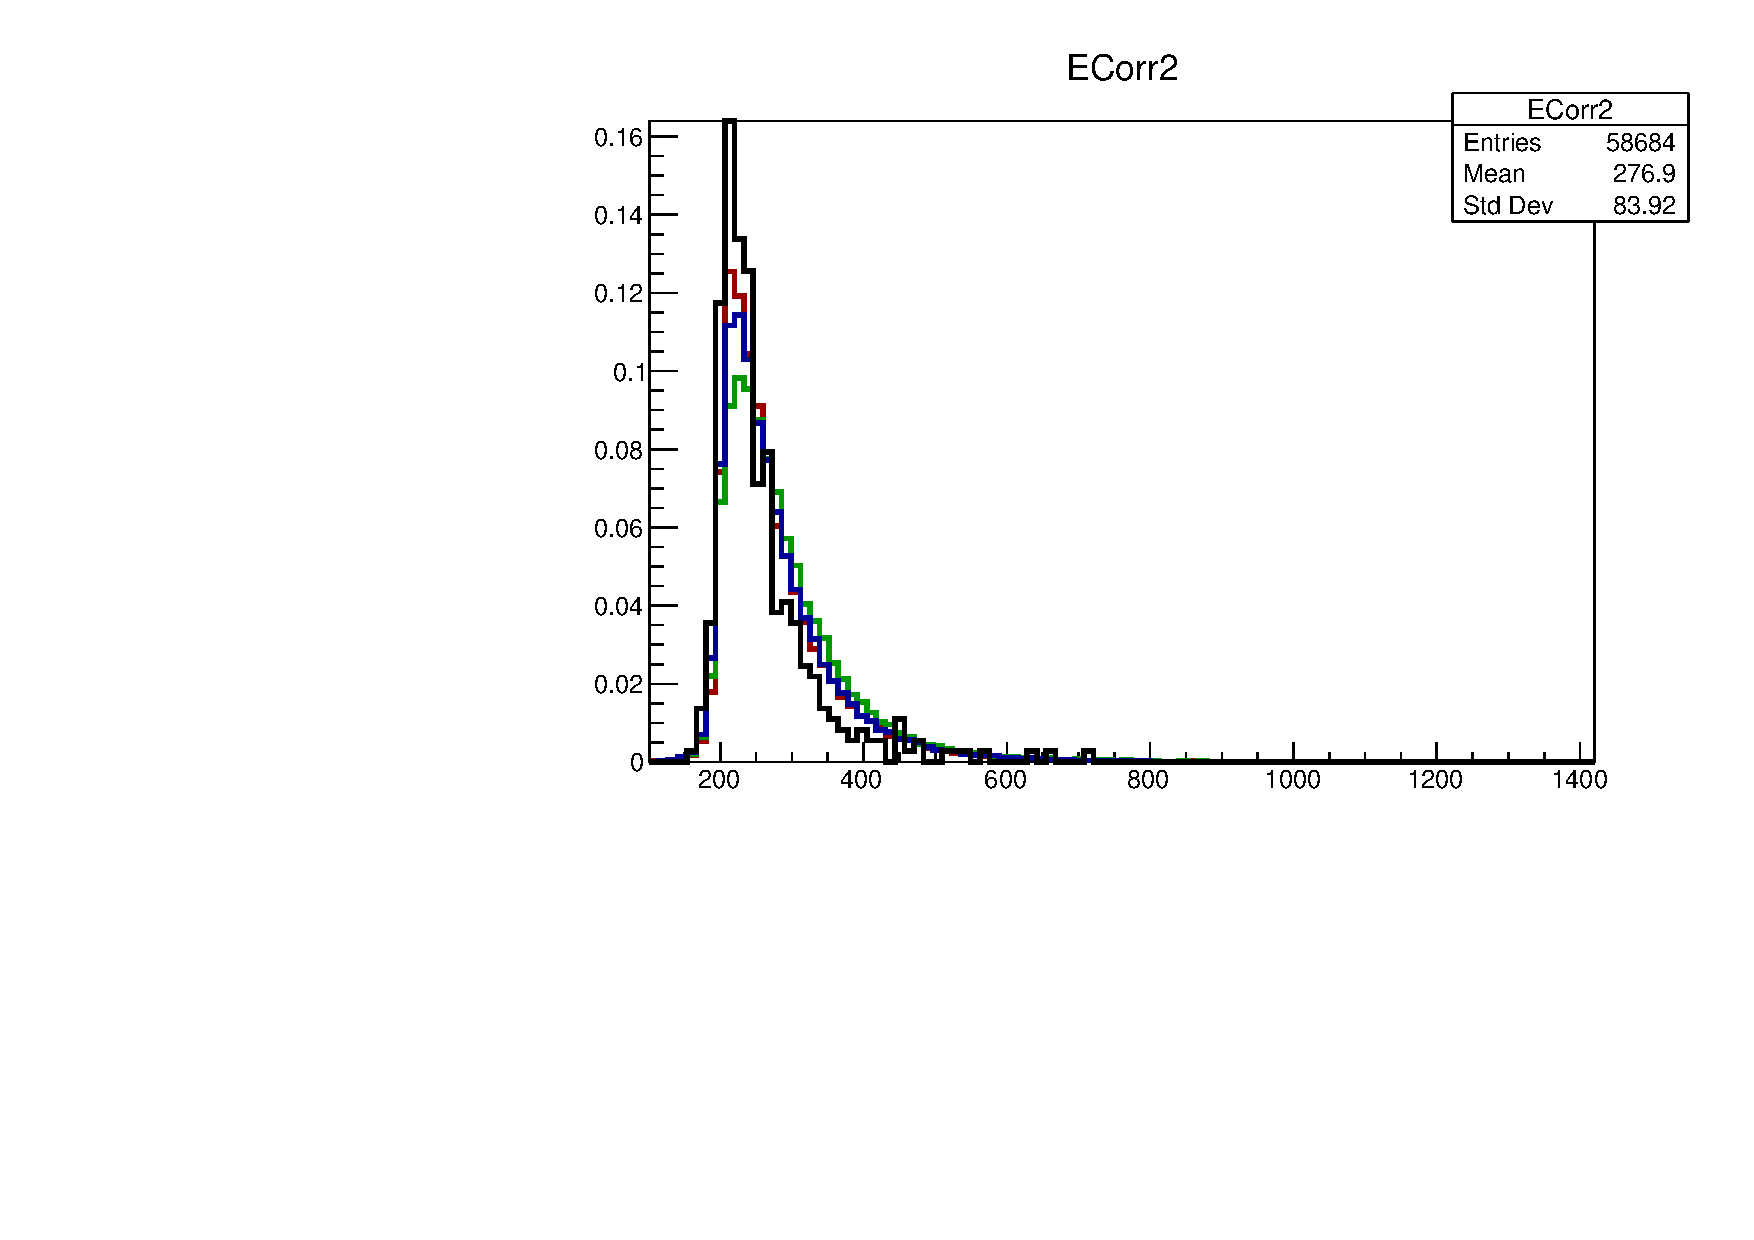
\includegraphics[width=0.49\textwidth]{./ECorr2.pdf}\\
        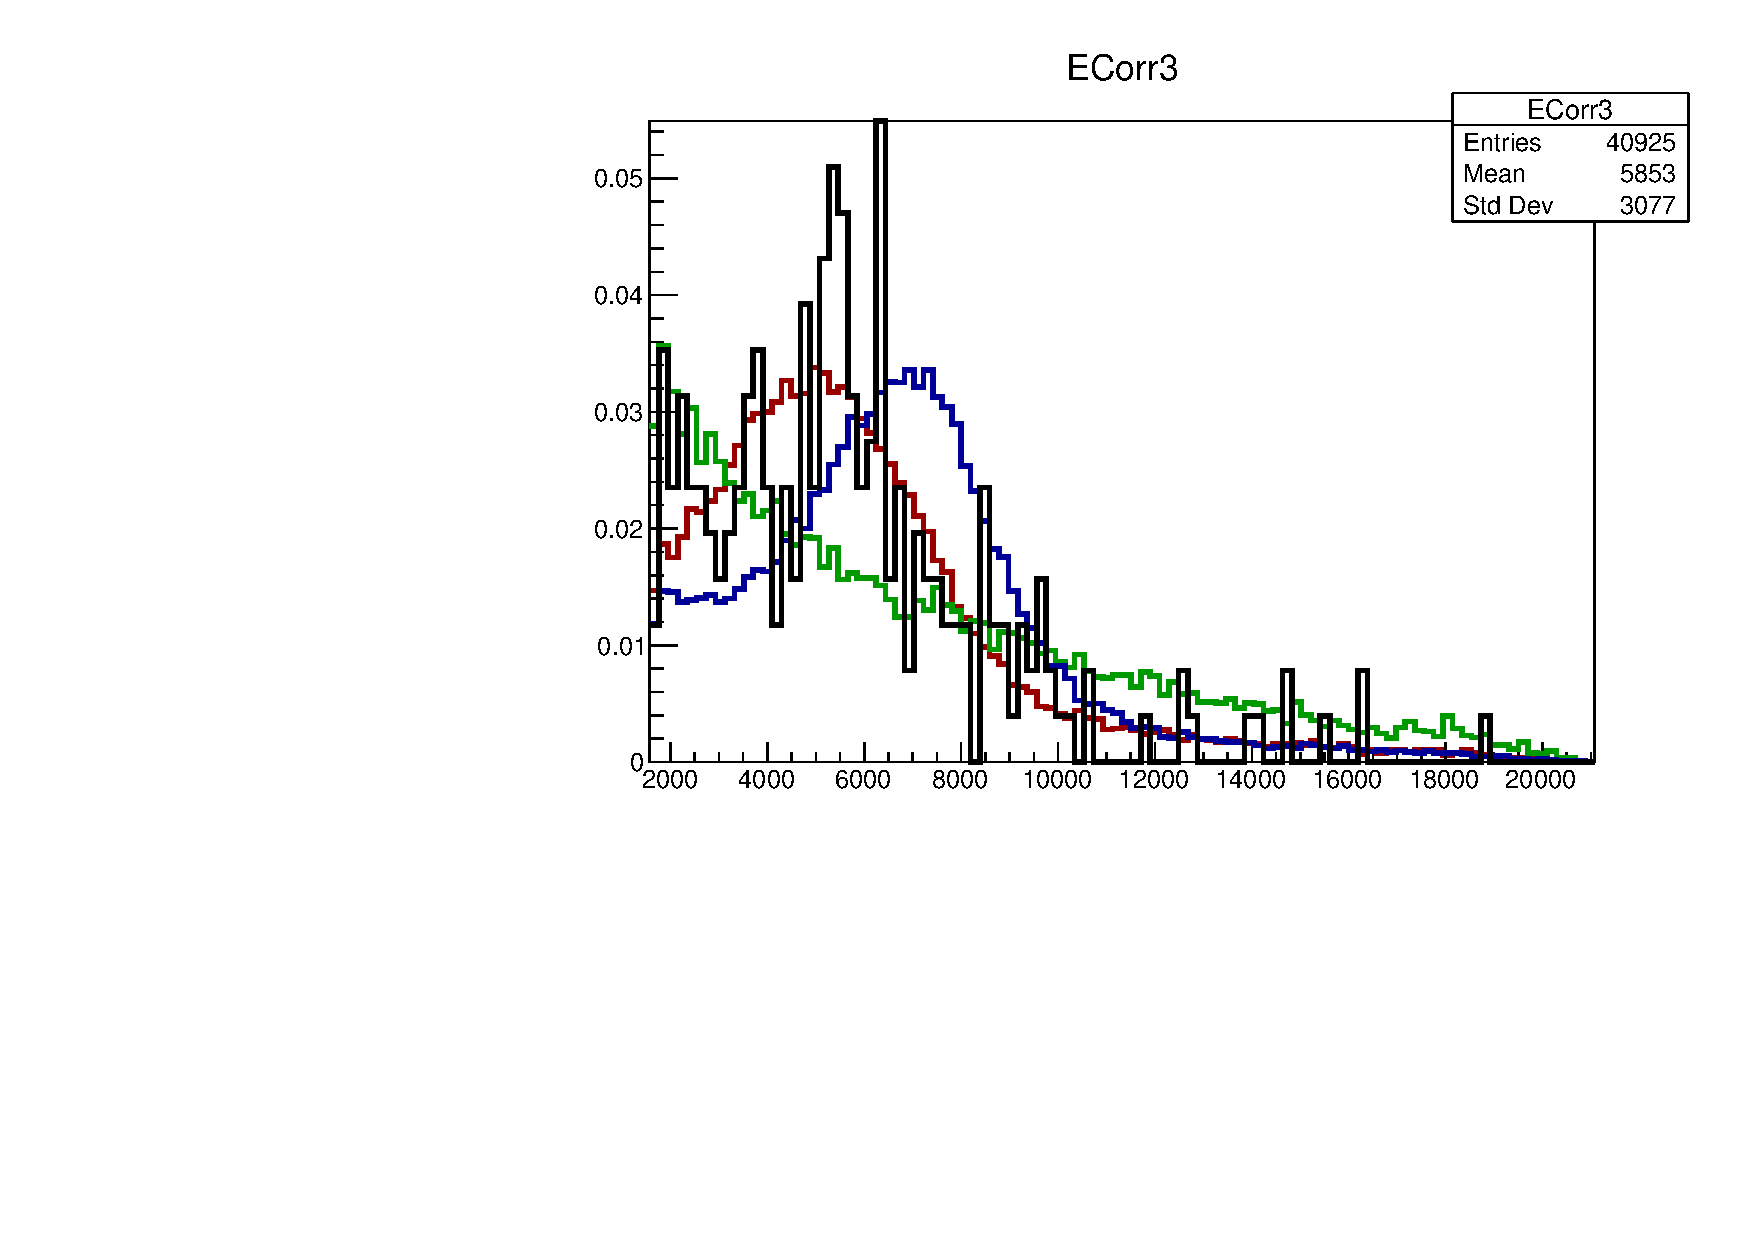
\includegraphics[width=0.49\textwidth]{./ECorr3.pdf}
        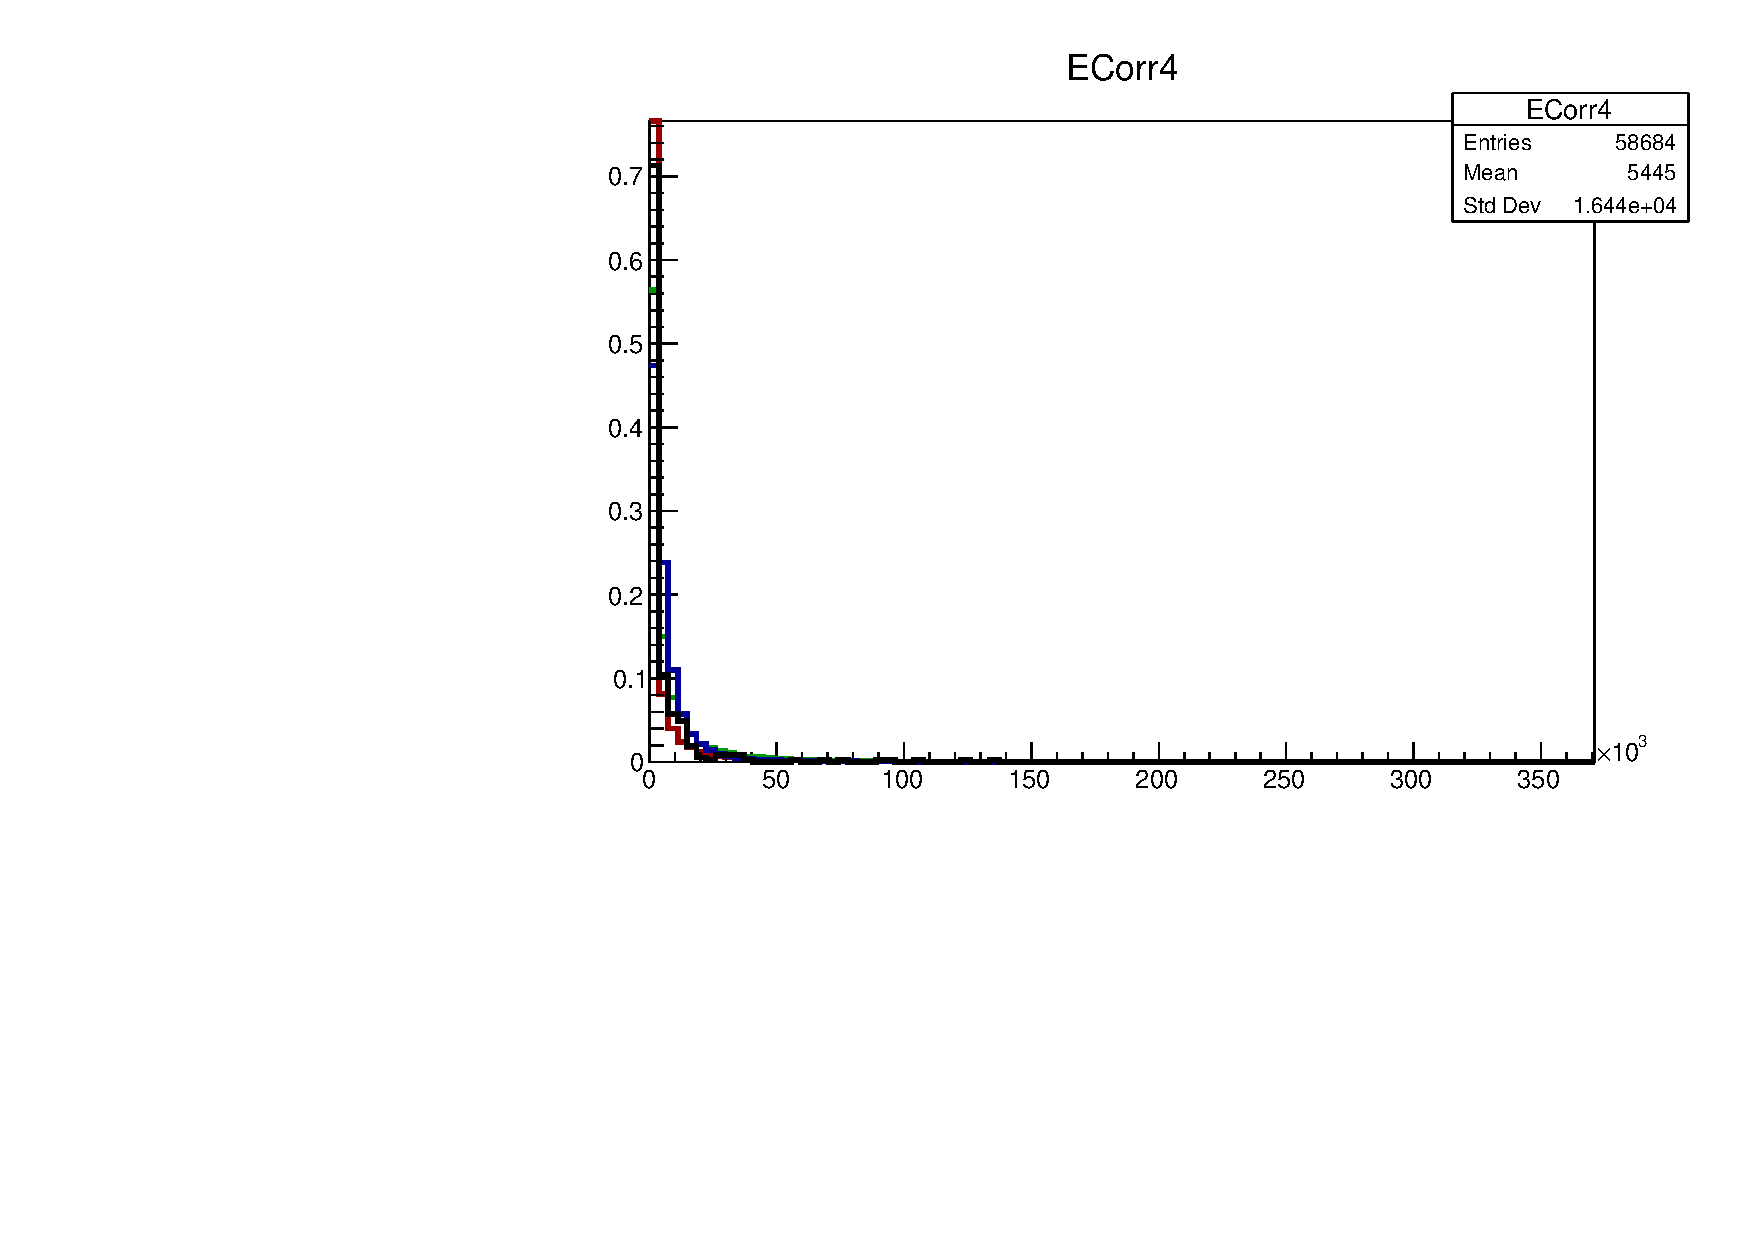
\includegraphics[width=0.49\textwidth]{./ECorr4.pdf}\\
        \includegraphics[width=0.49\textwidth]{./ECorr5.pdf}
        \includegraphics[width=0.49\textwidth]{./ECorr6.pdf}\\
        \caption{ Energy Correlation observable, normalized to unit area under the curve. }
        \label{fig:ECorr}
    \end{center}
\end{figure}

\begin{figure}[H]
    \begin{center}
        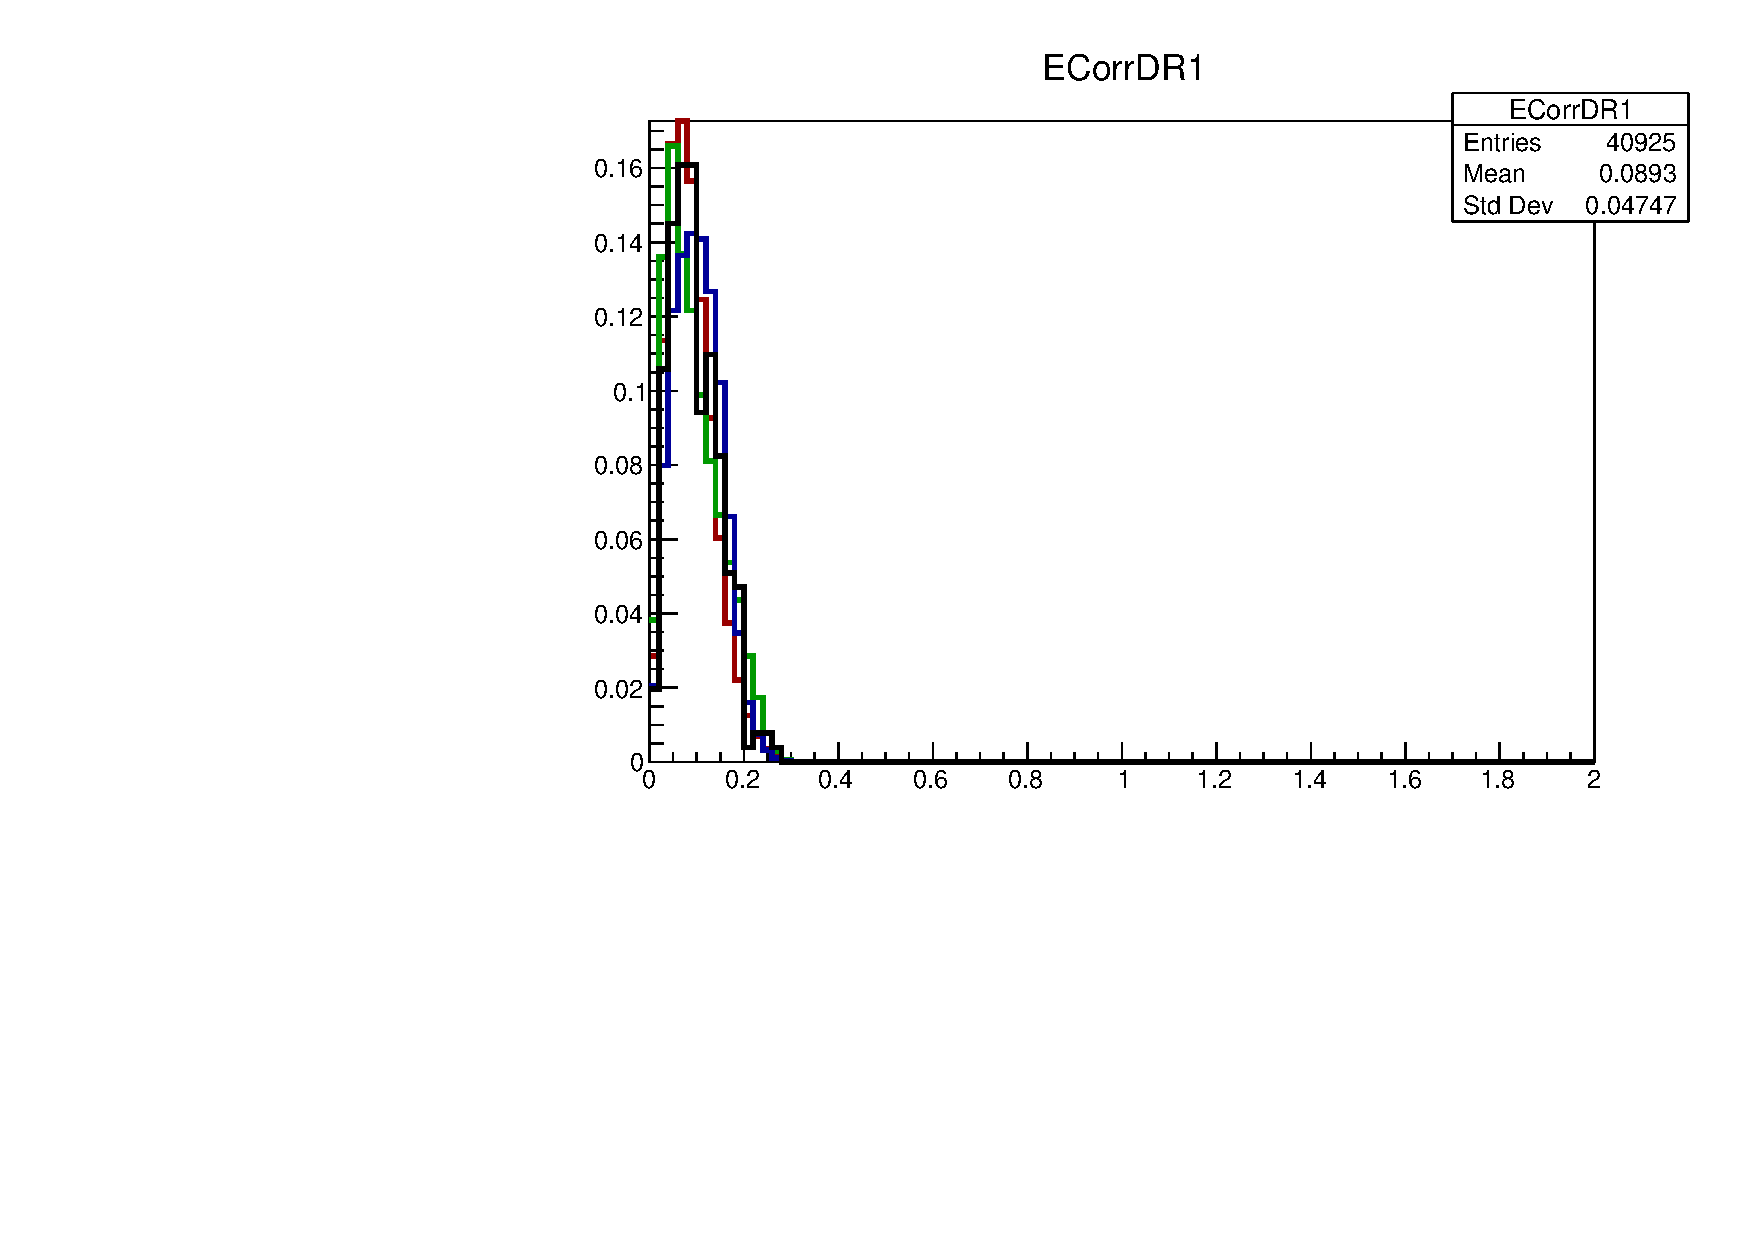
\includegraphics[width=0.49\textwidth]{./ECorrDR1.pdf}
        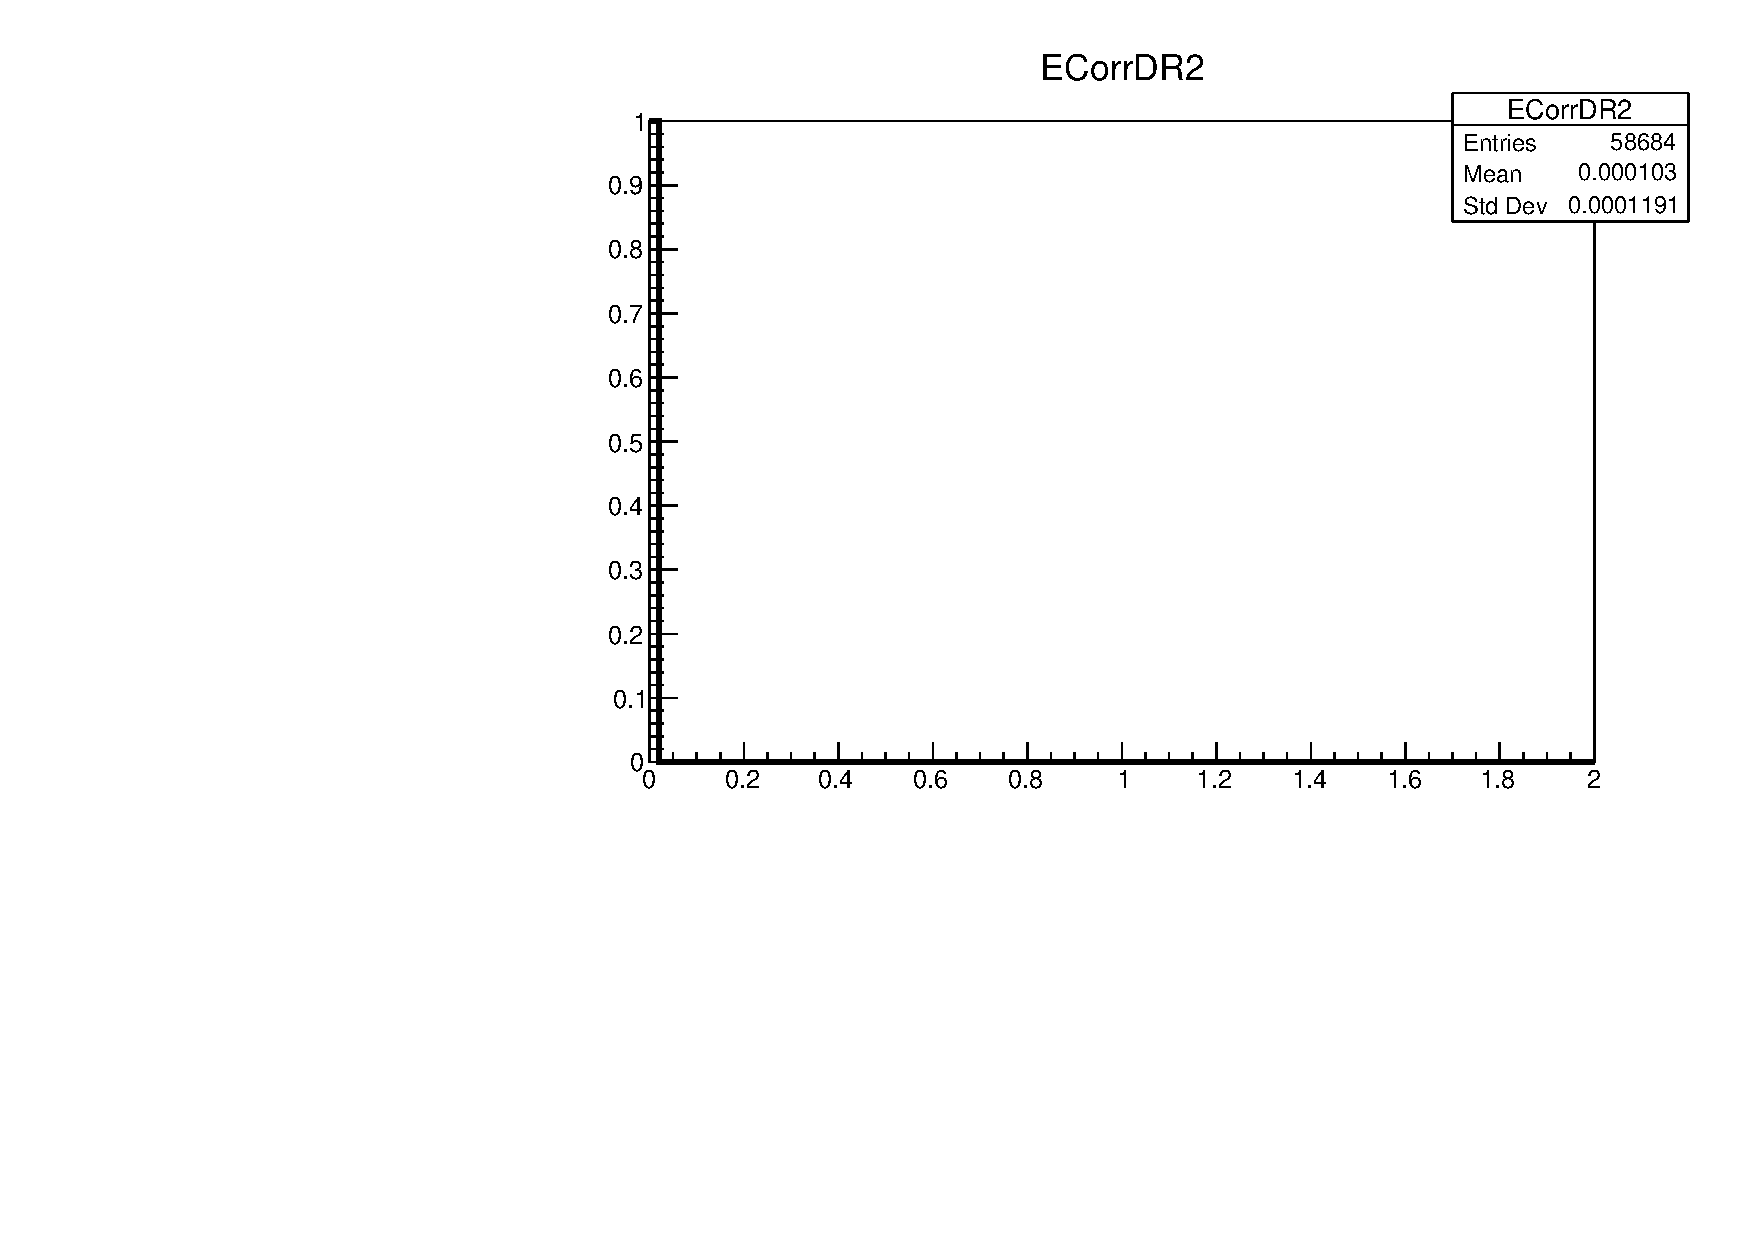
\includegraphics[width=0.49\textwidth]{./ECorrDR2.pdf}\\
        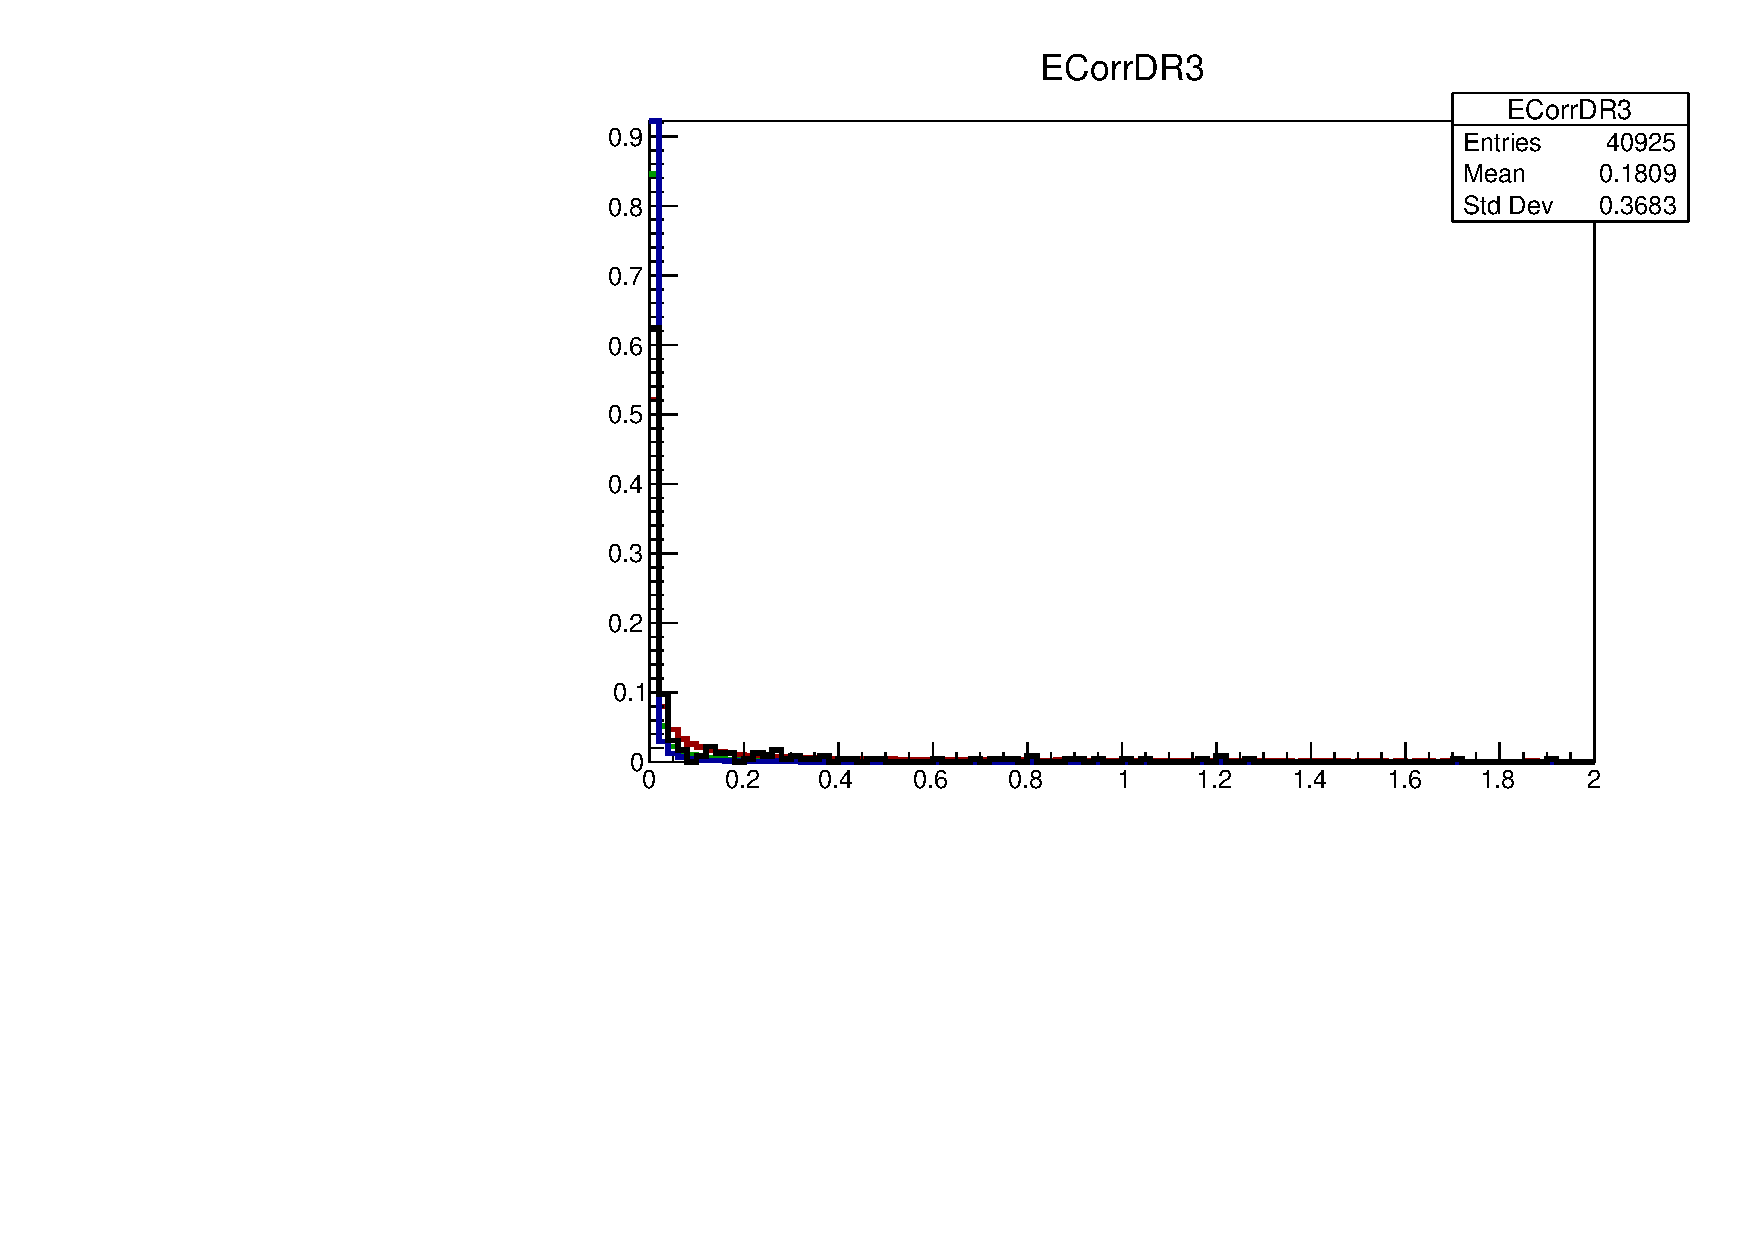
\includegraphics[width=0.49\textwidth]{./ECorrDR3.pdf}
        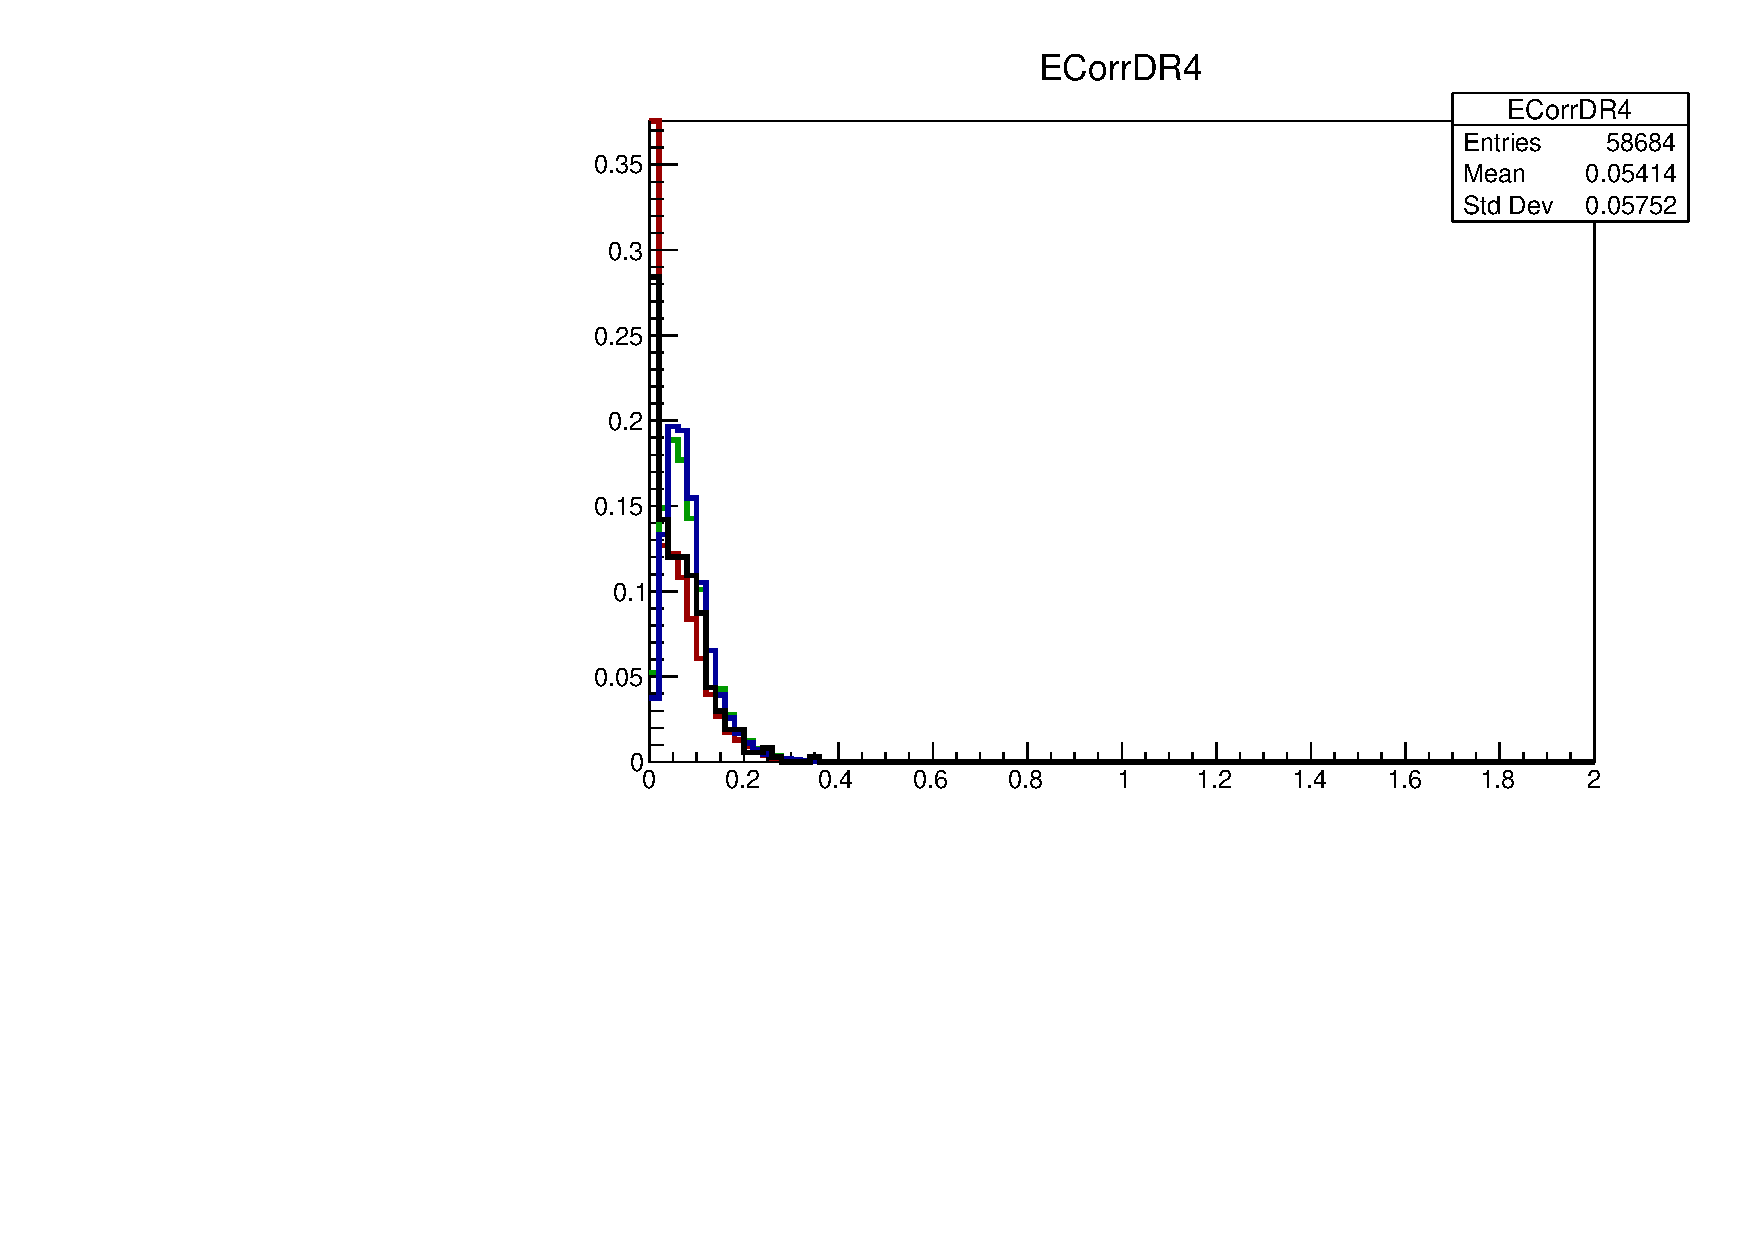
\includegraphics[width=0.49\textwidth]{./ECorrDR4.pdf}\\
        \caption{ Energy Correlation double ratio observable, normalized to unit area under the curve. }
        \label{fig:ECorrDR}
    \end{center}
\end{figure}

\begin{figure}[H]
    \begin{center}
        \includegraphics[width=0.49\textwidth]{./T1NSub1vsPf.pdf}
        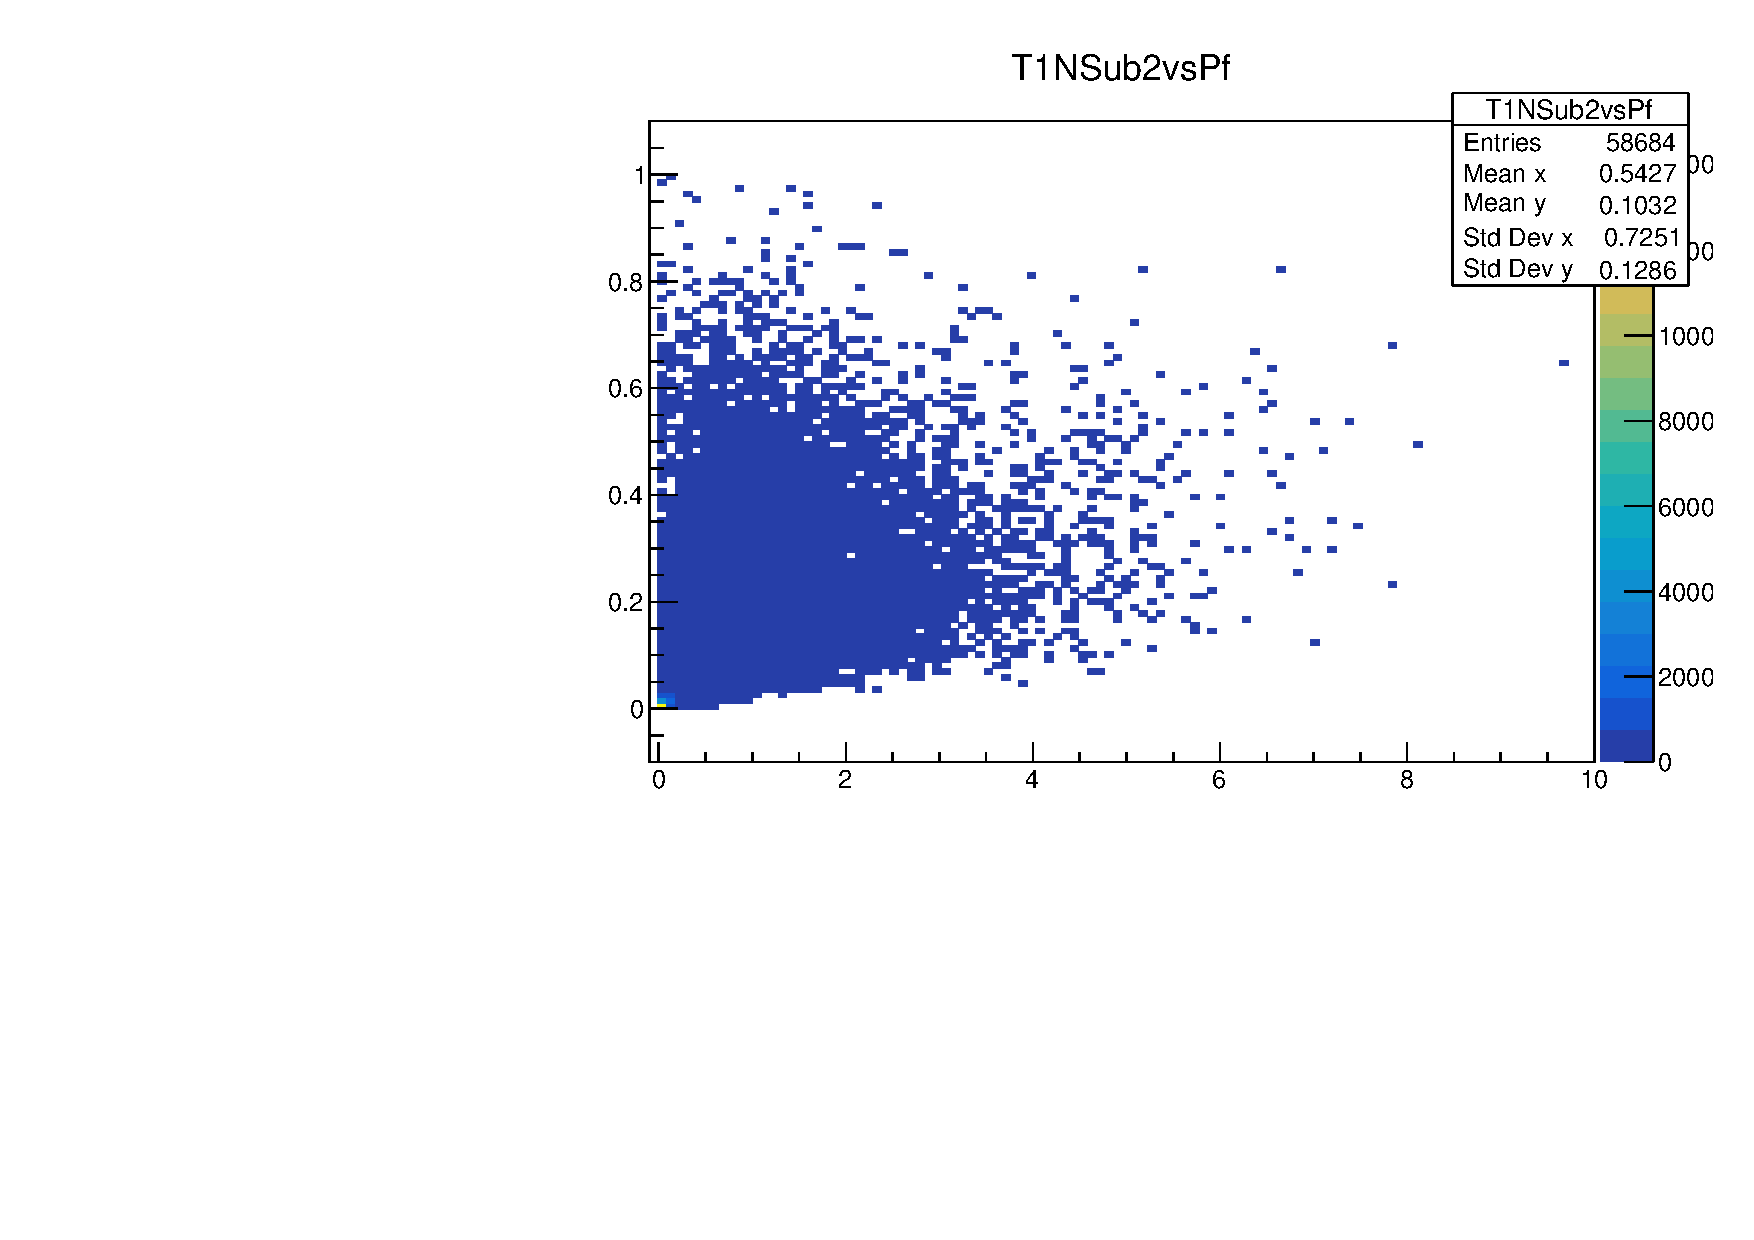
\includegraphics[width=0.49\textwidth]{./T1NSub2vsPf.pdf}\\
        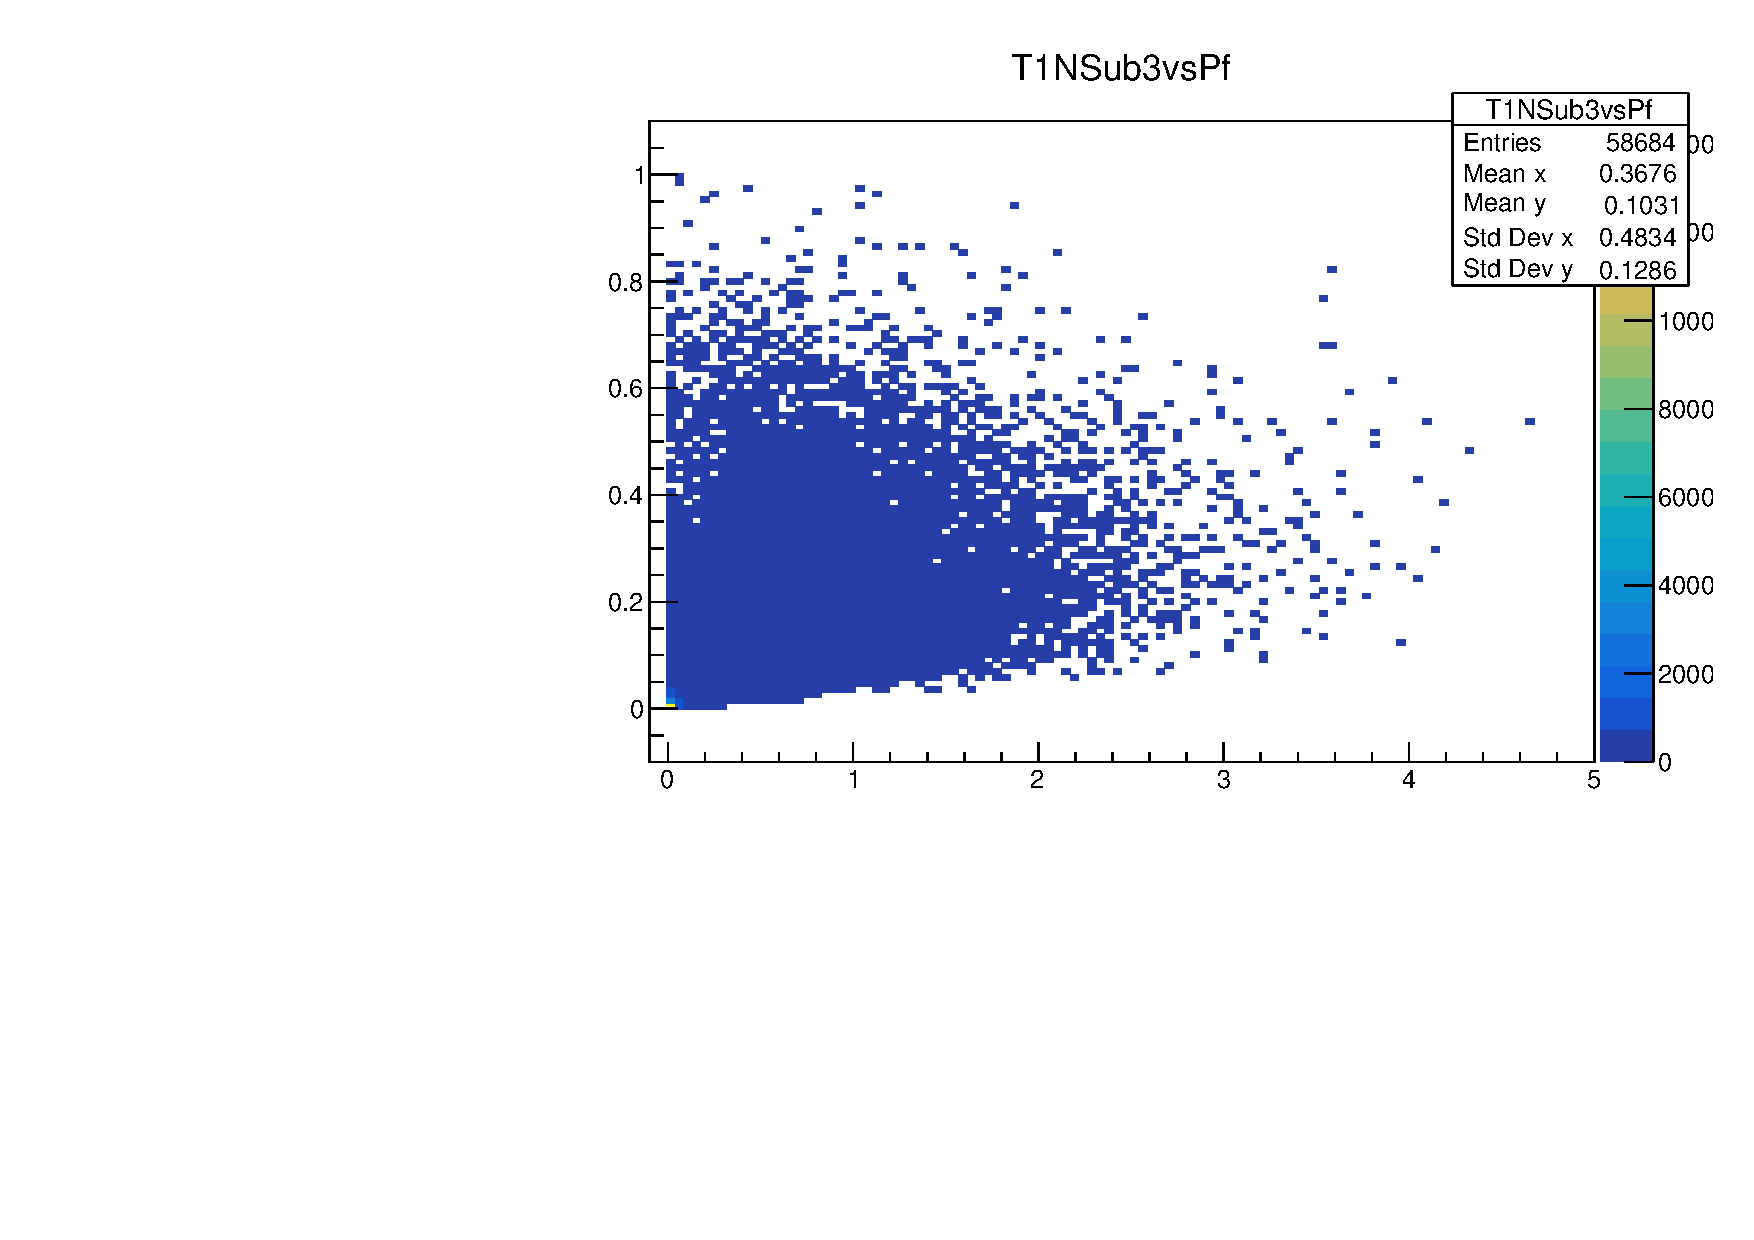
\includegraphics[width=0.49\textwidth]{./T1NSub3vsPf.pdf}
        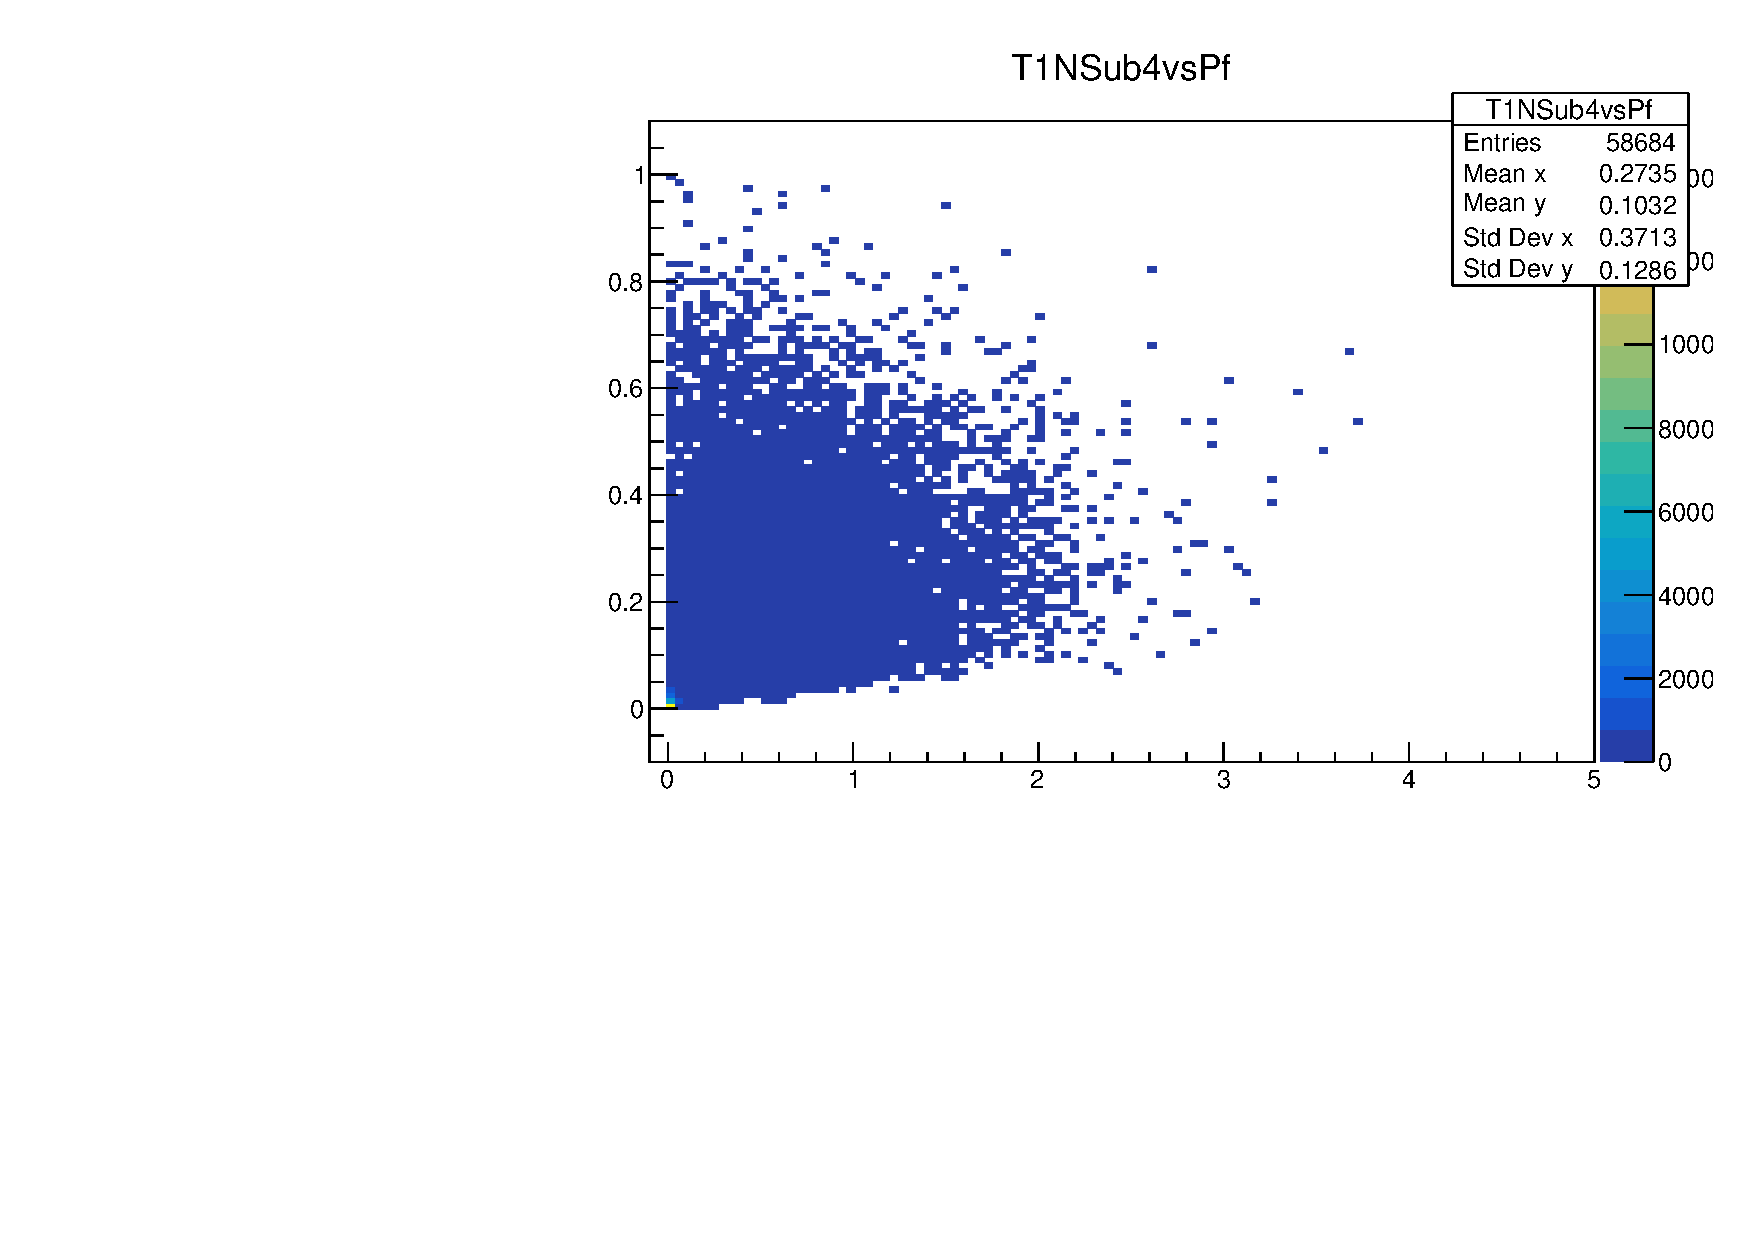
\includegraphics[width=0.49\textwidth]{./T1NSub4vsPf.pdf}\\
        \caption{ {\tt NSubjettiness} (x-axis) vs planar flow (y-axis) for boosted $jZ\rightarrow \tau \bar{\tau}$ }
        \label{fig:nsubvspf1}
    \end{center}
\end{figure}

\begin{figure}[H]
    \begin{center}
        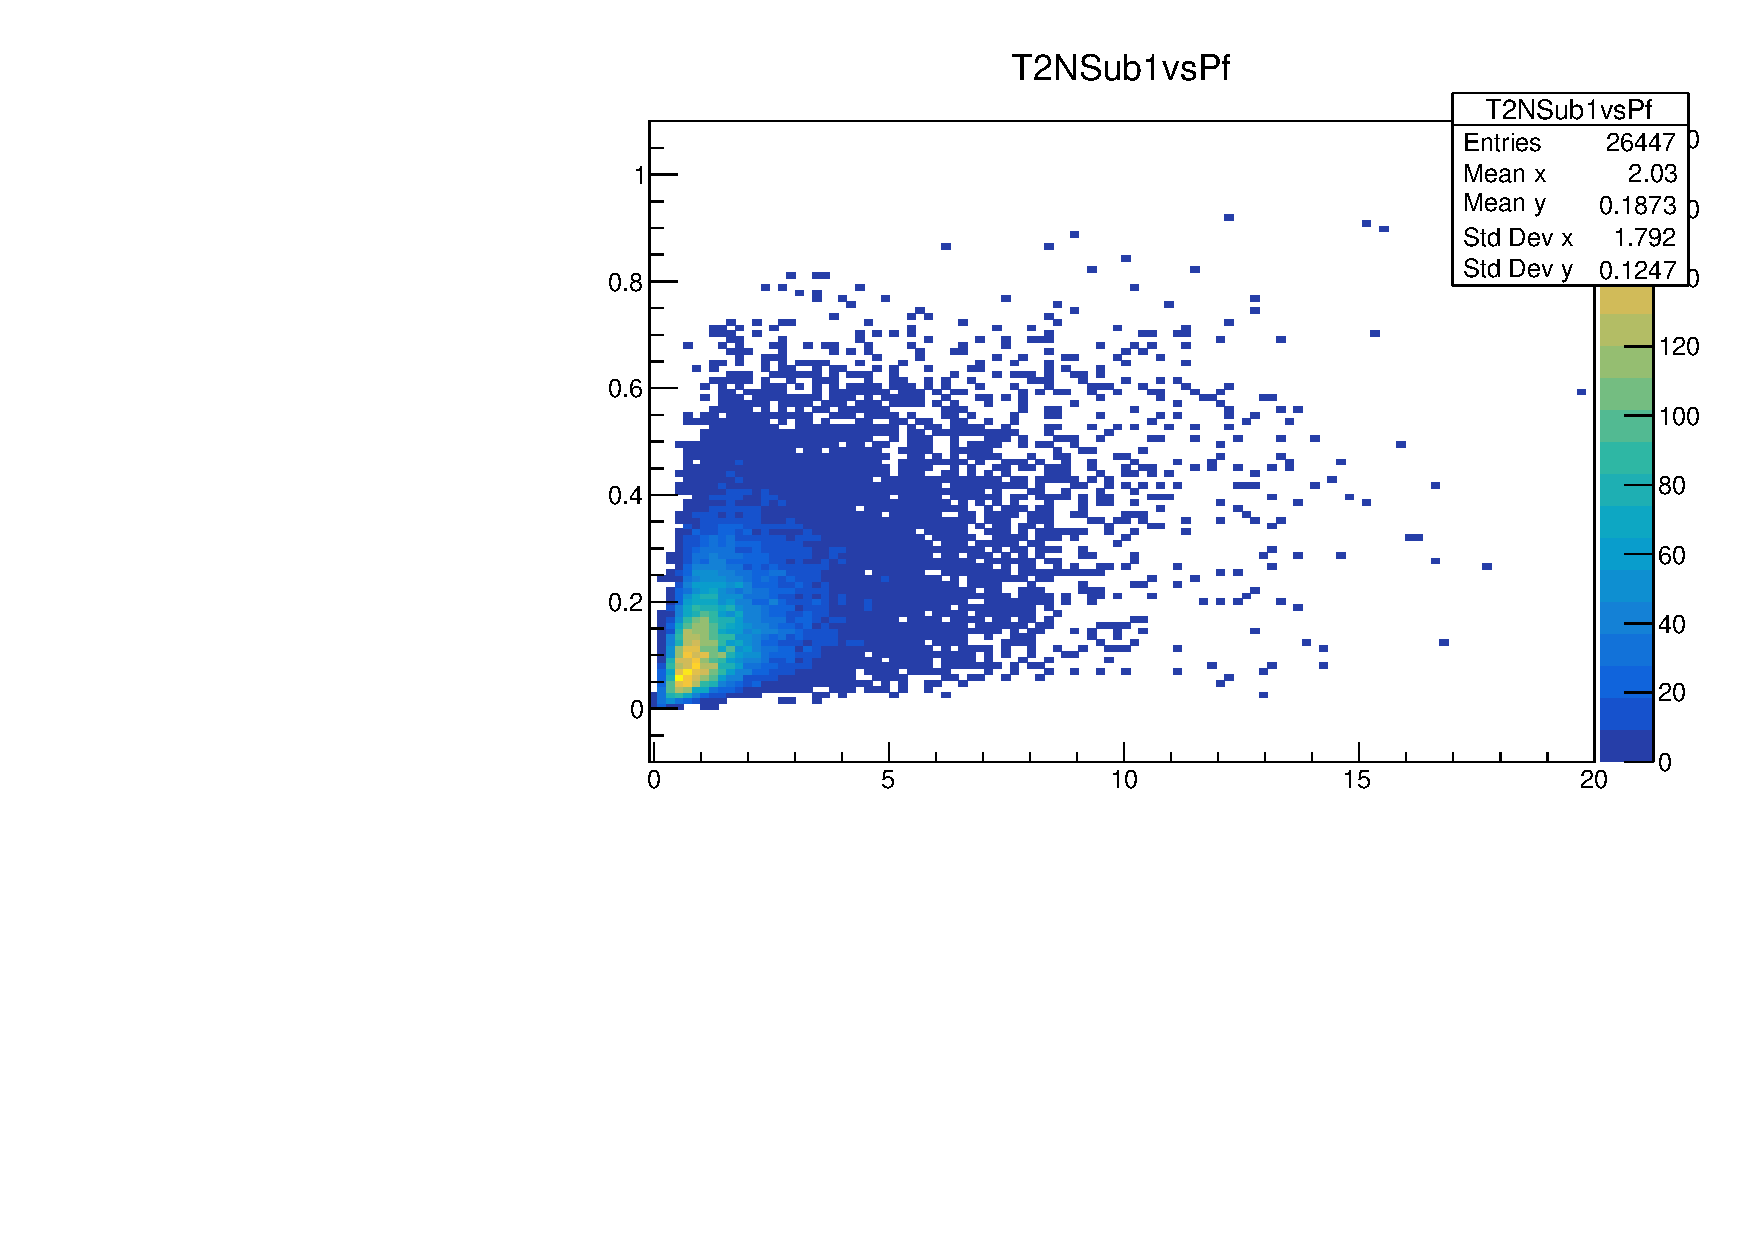
\includegraphics[width=0.49\textwidth]{./T2NSub1vsPf.pdf}
        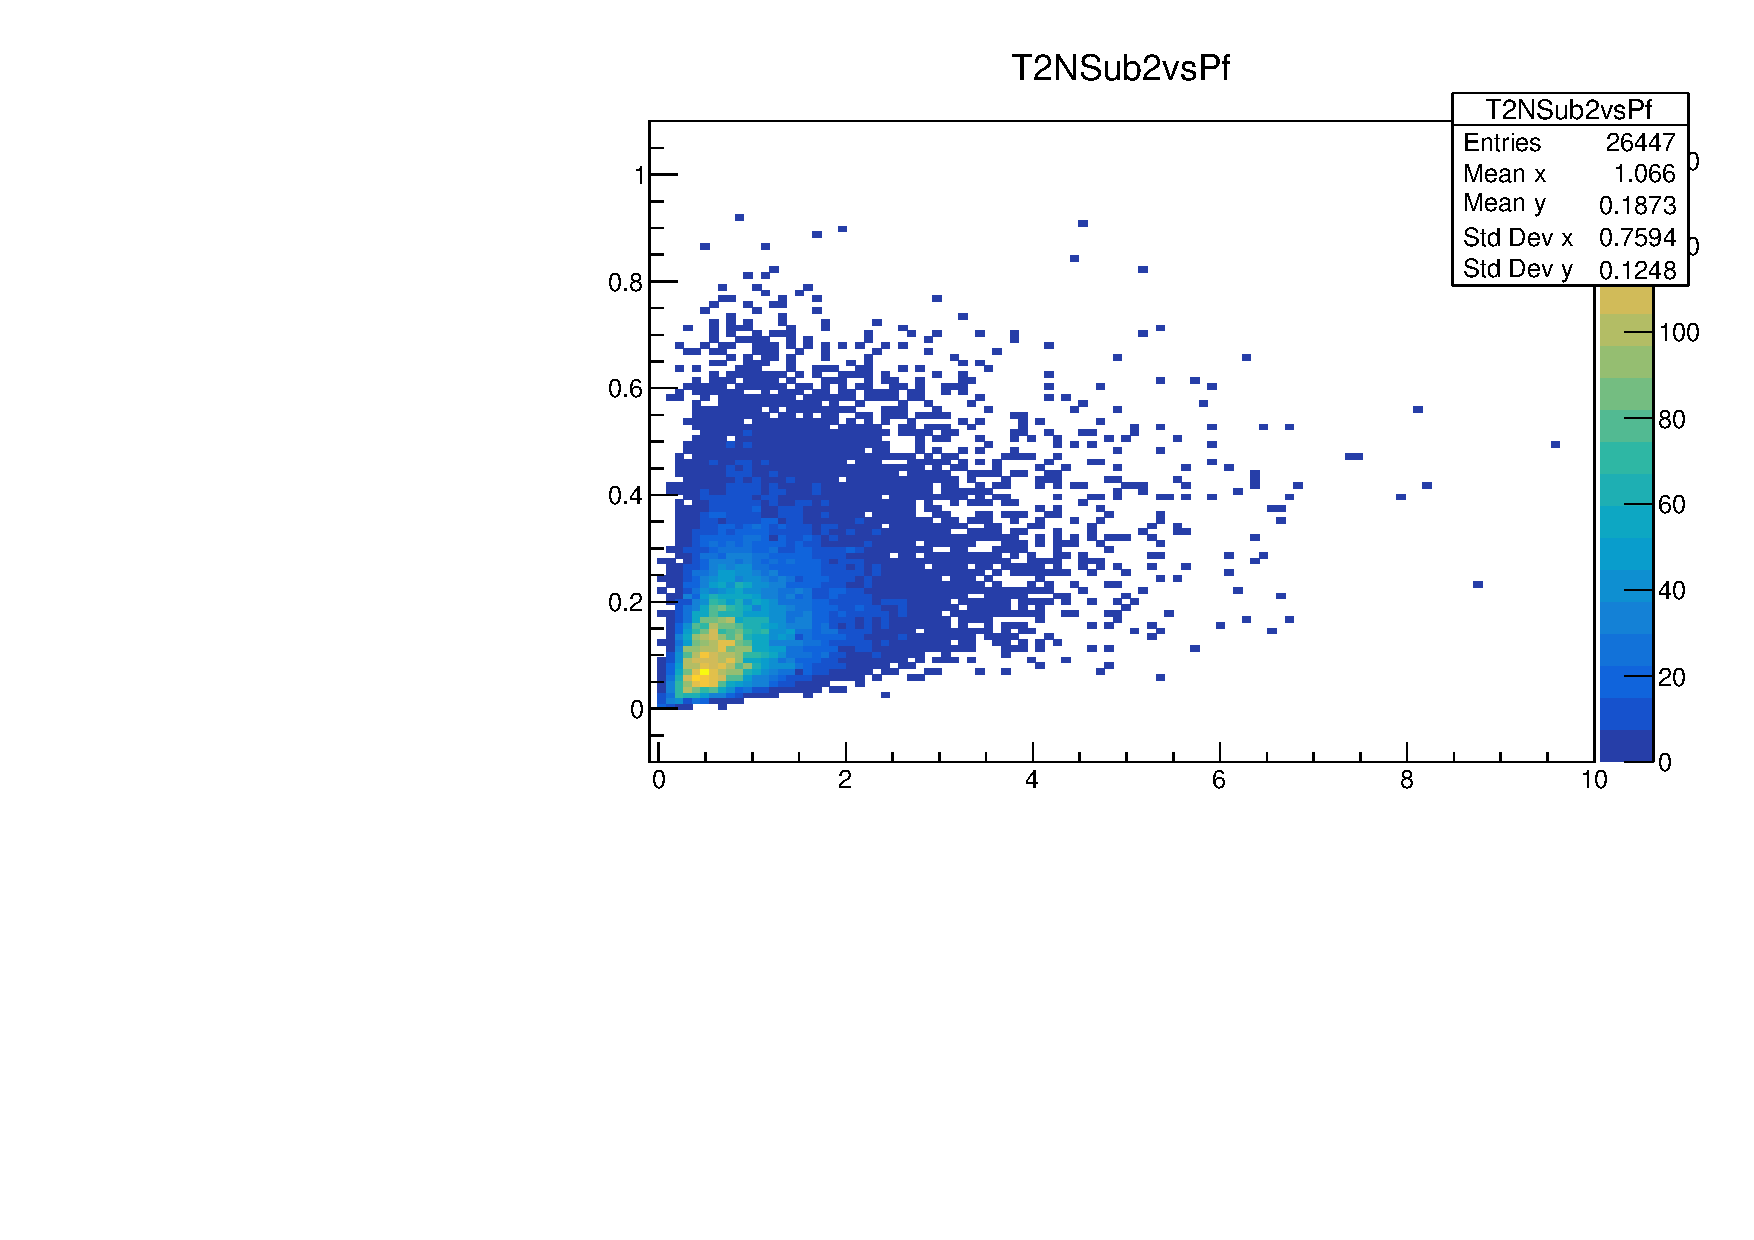
\includegraphics[width=0.49\textwidth]{./T2NSub2vsPf.pdf}\\
        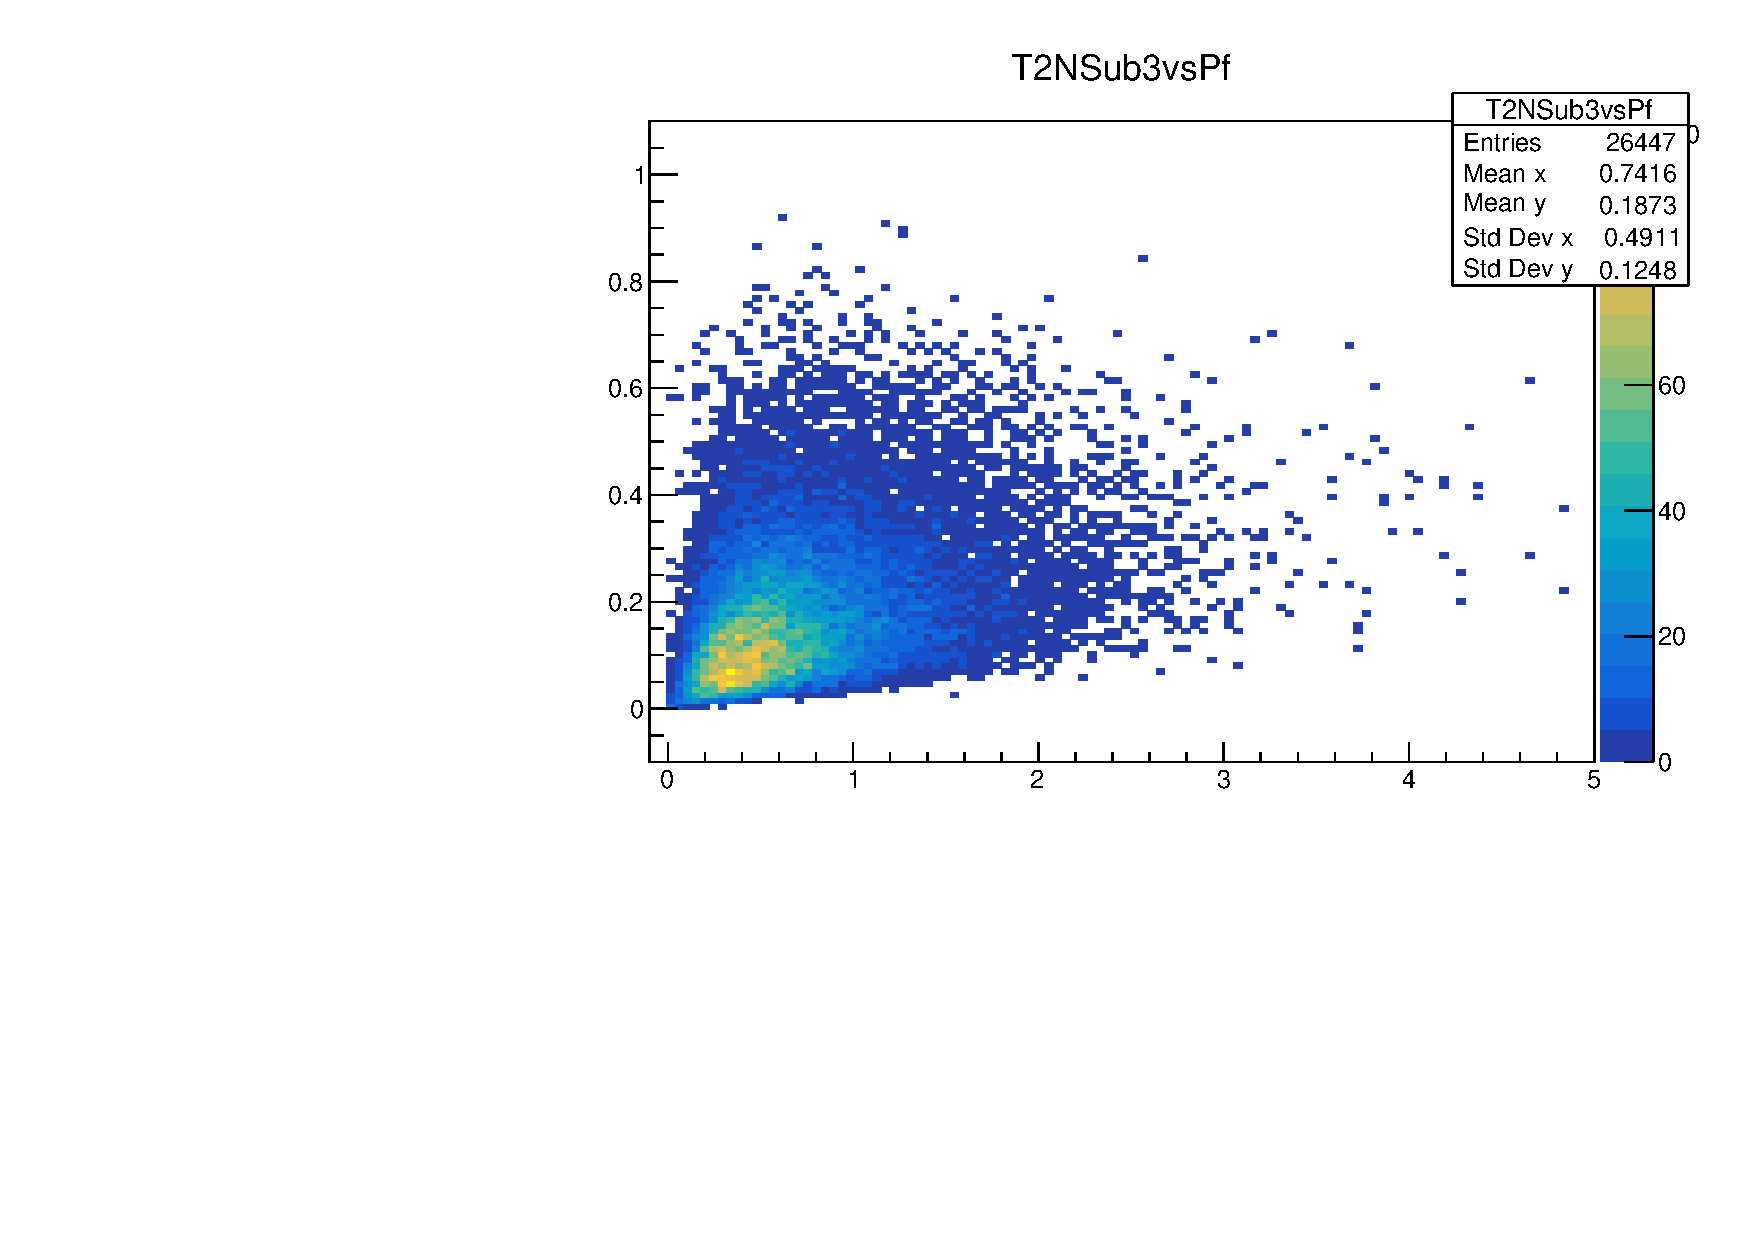
\includegraphics[width=0.49\textwidth]{./T2NSub3vsPf.pdf}
        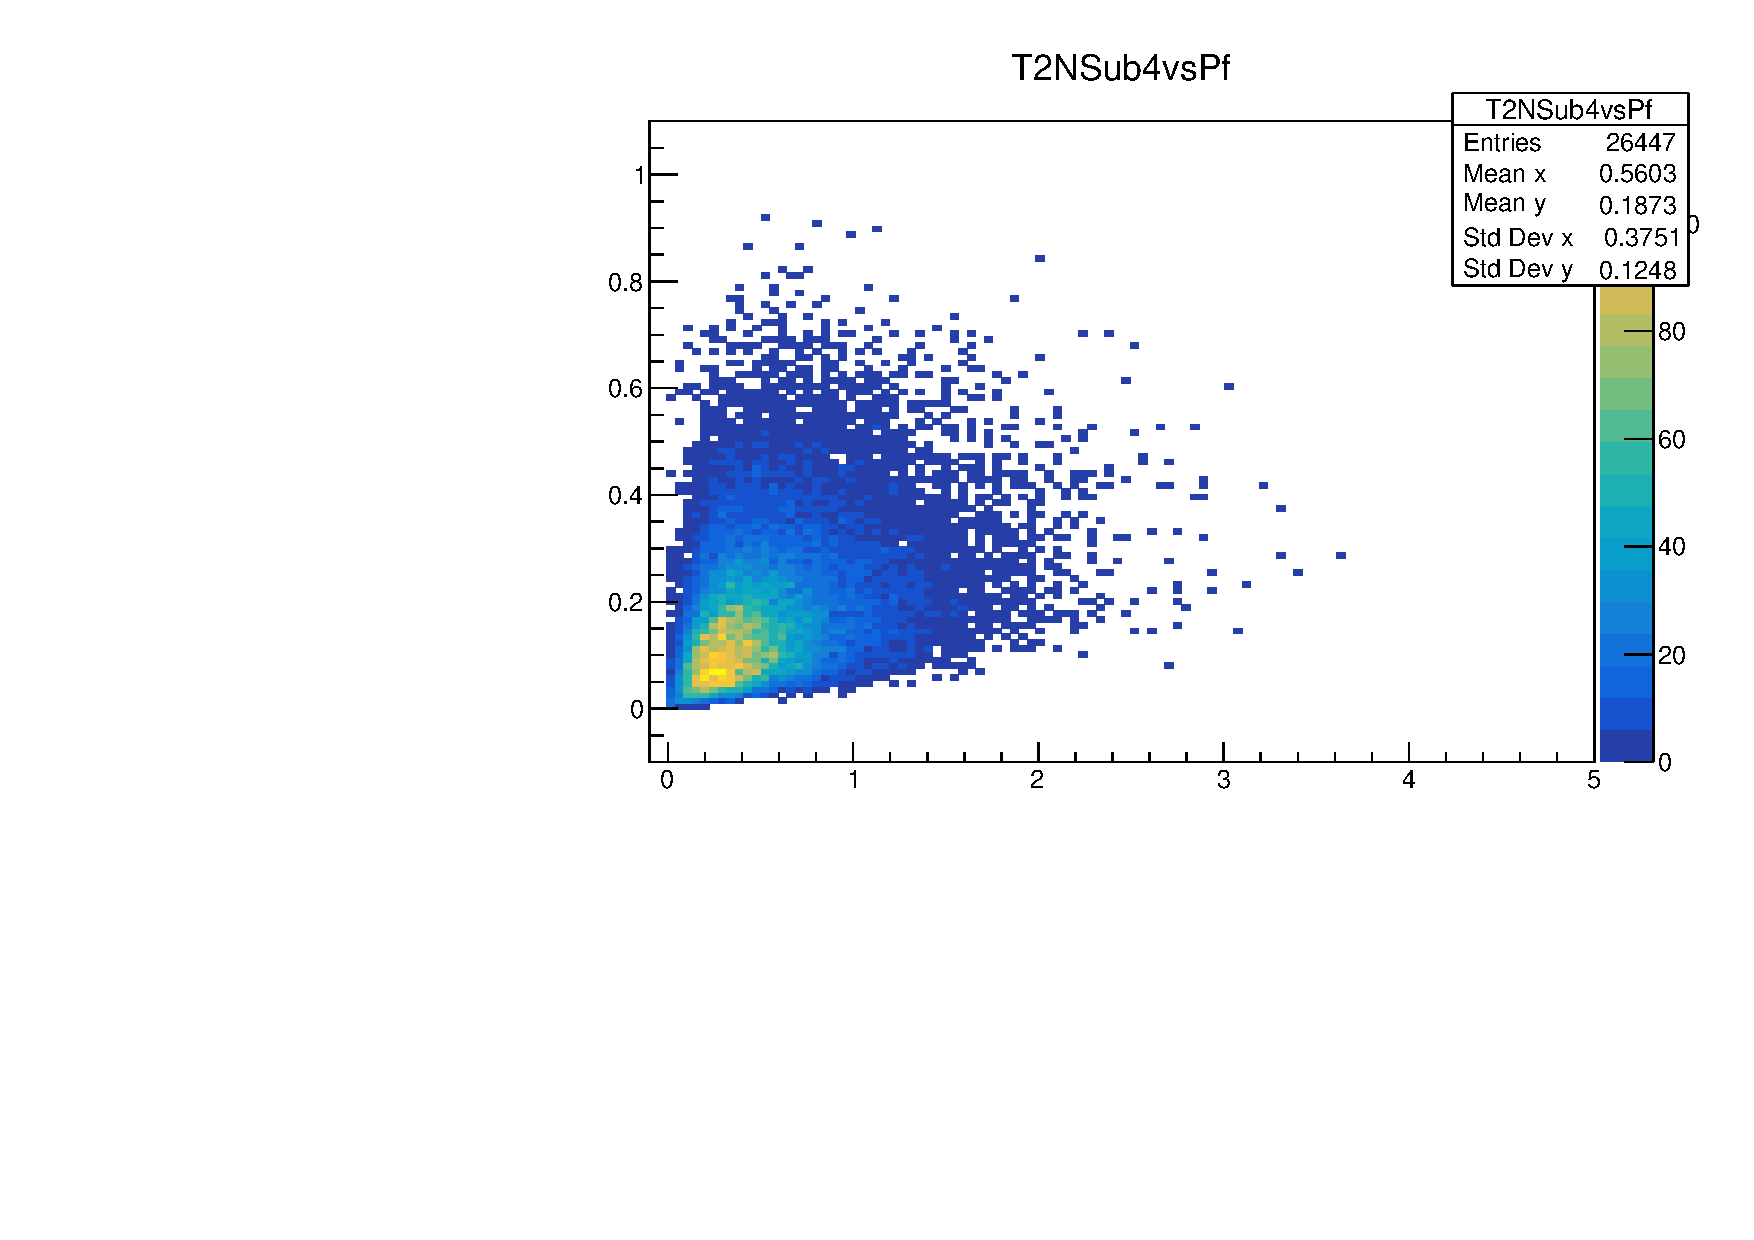
\includegraphics[width=0.49\textwidth]{./T2NSub4vsPf.pdf}\\
        \caption{ {\tt NSubjettiness} (x-axis) vs planar flow (y-axis) for boosted $jZ\rightarrow \nu \bar{\nu}$ }
        \label{fig:nsubvspf2}
    \end{center}
\end{figure}

\begin{figure}[H]
    \begin{center}
        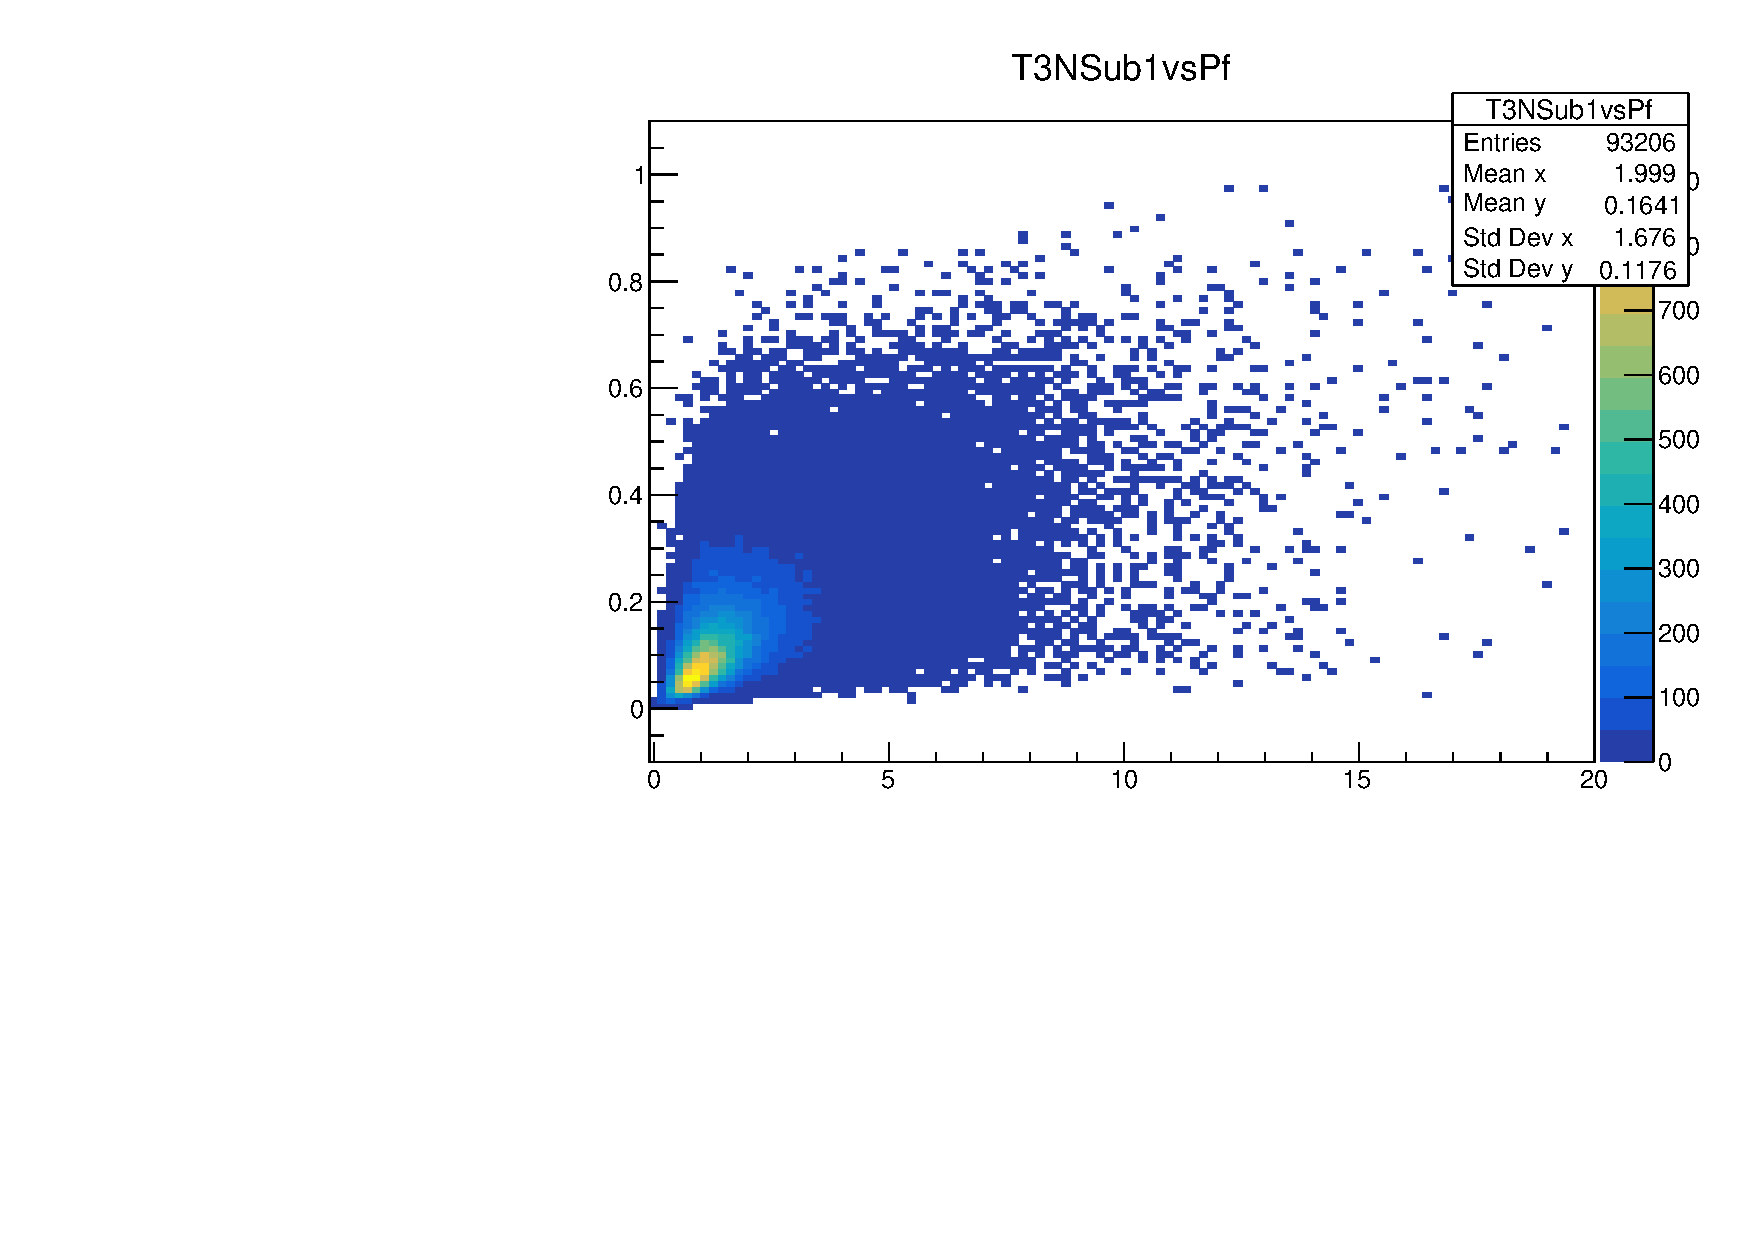
\includegraphics[width=0.49\textwidth]{./T3NSub1vsPf.pdf}
        \includegraphics[width=0.49\textwidth]{./T3NSub2vsPf.pdf}\\
        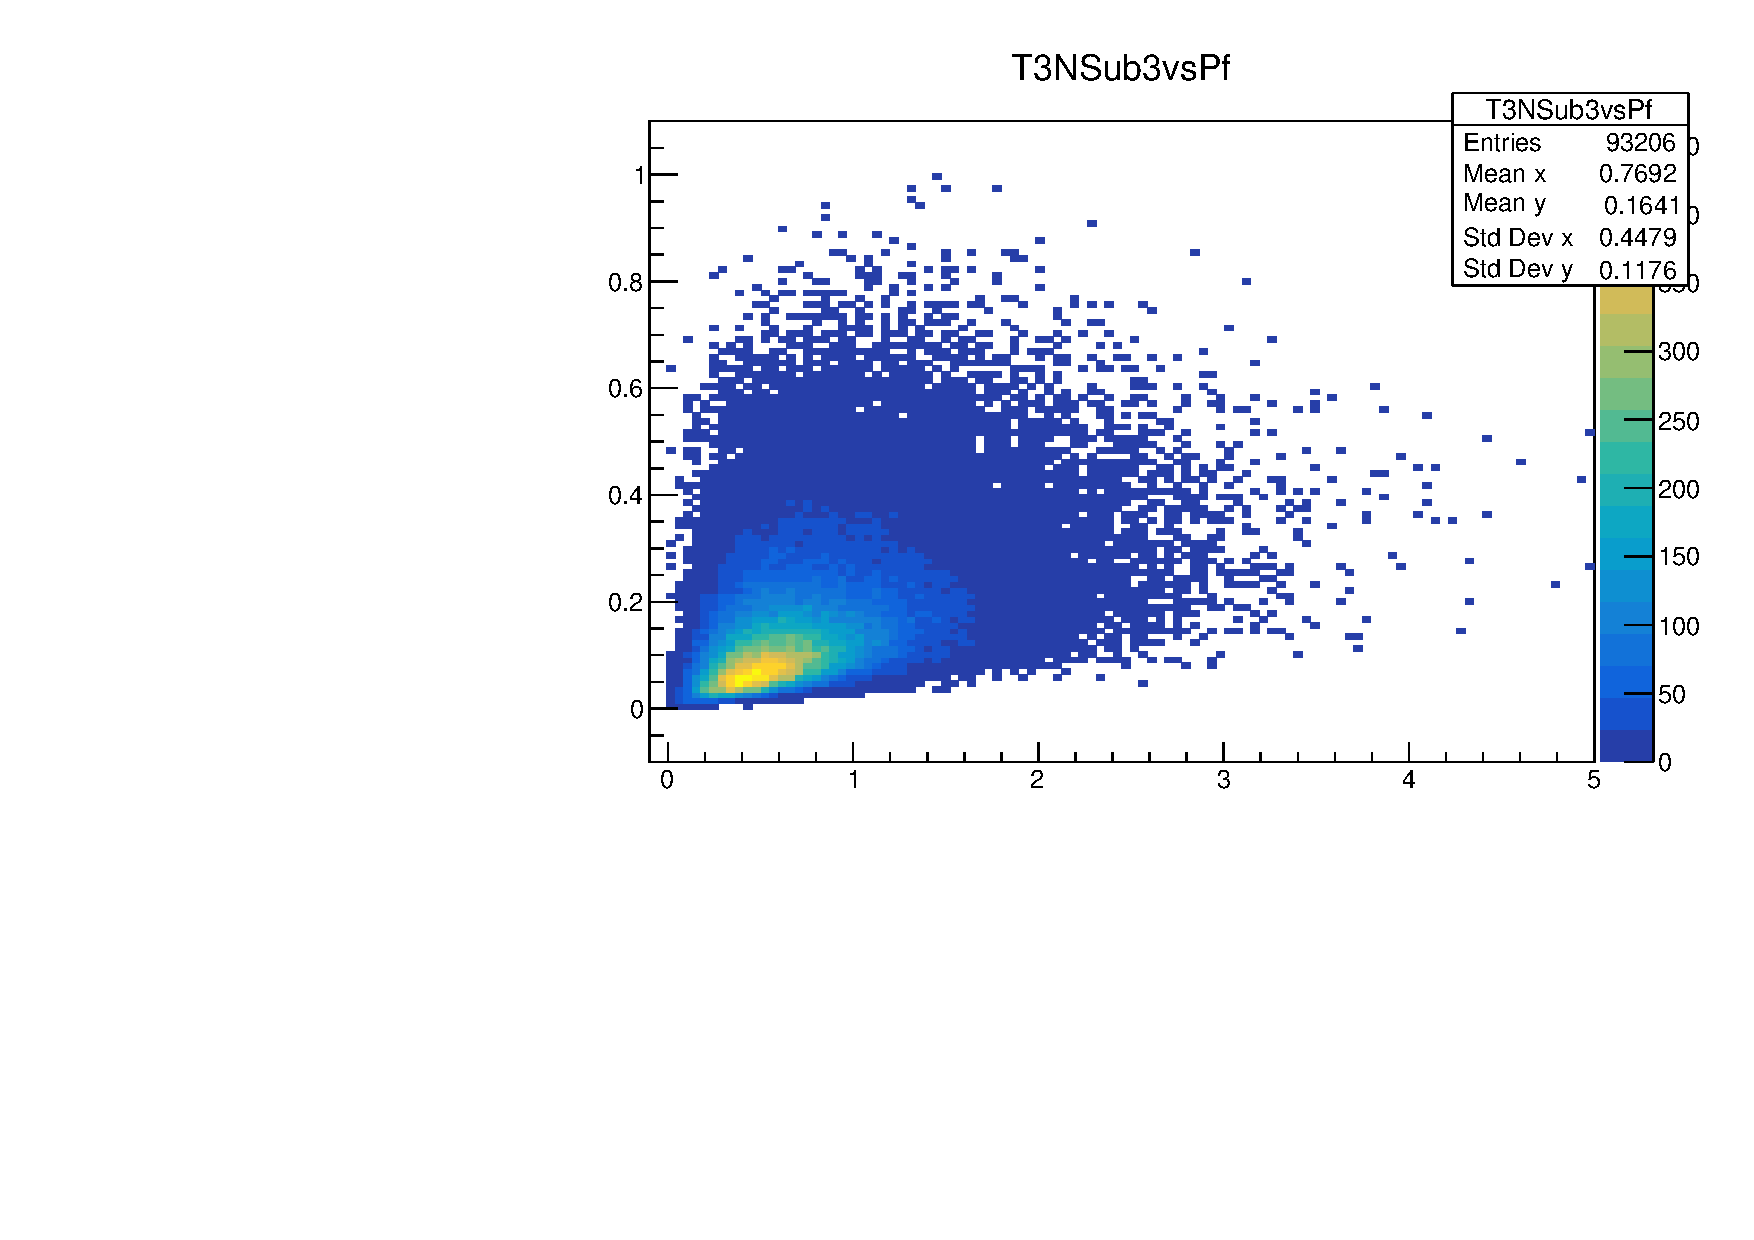
\includegraphics[width=0.49\textwidth]{./T3NSub3vsPf.pdf}
        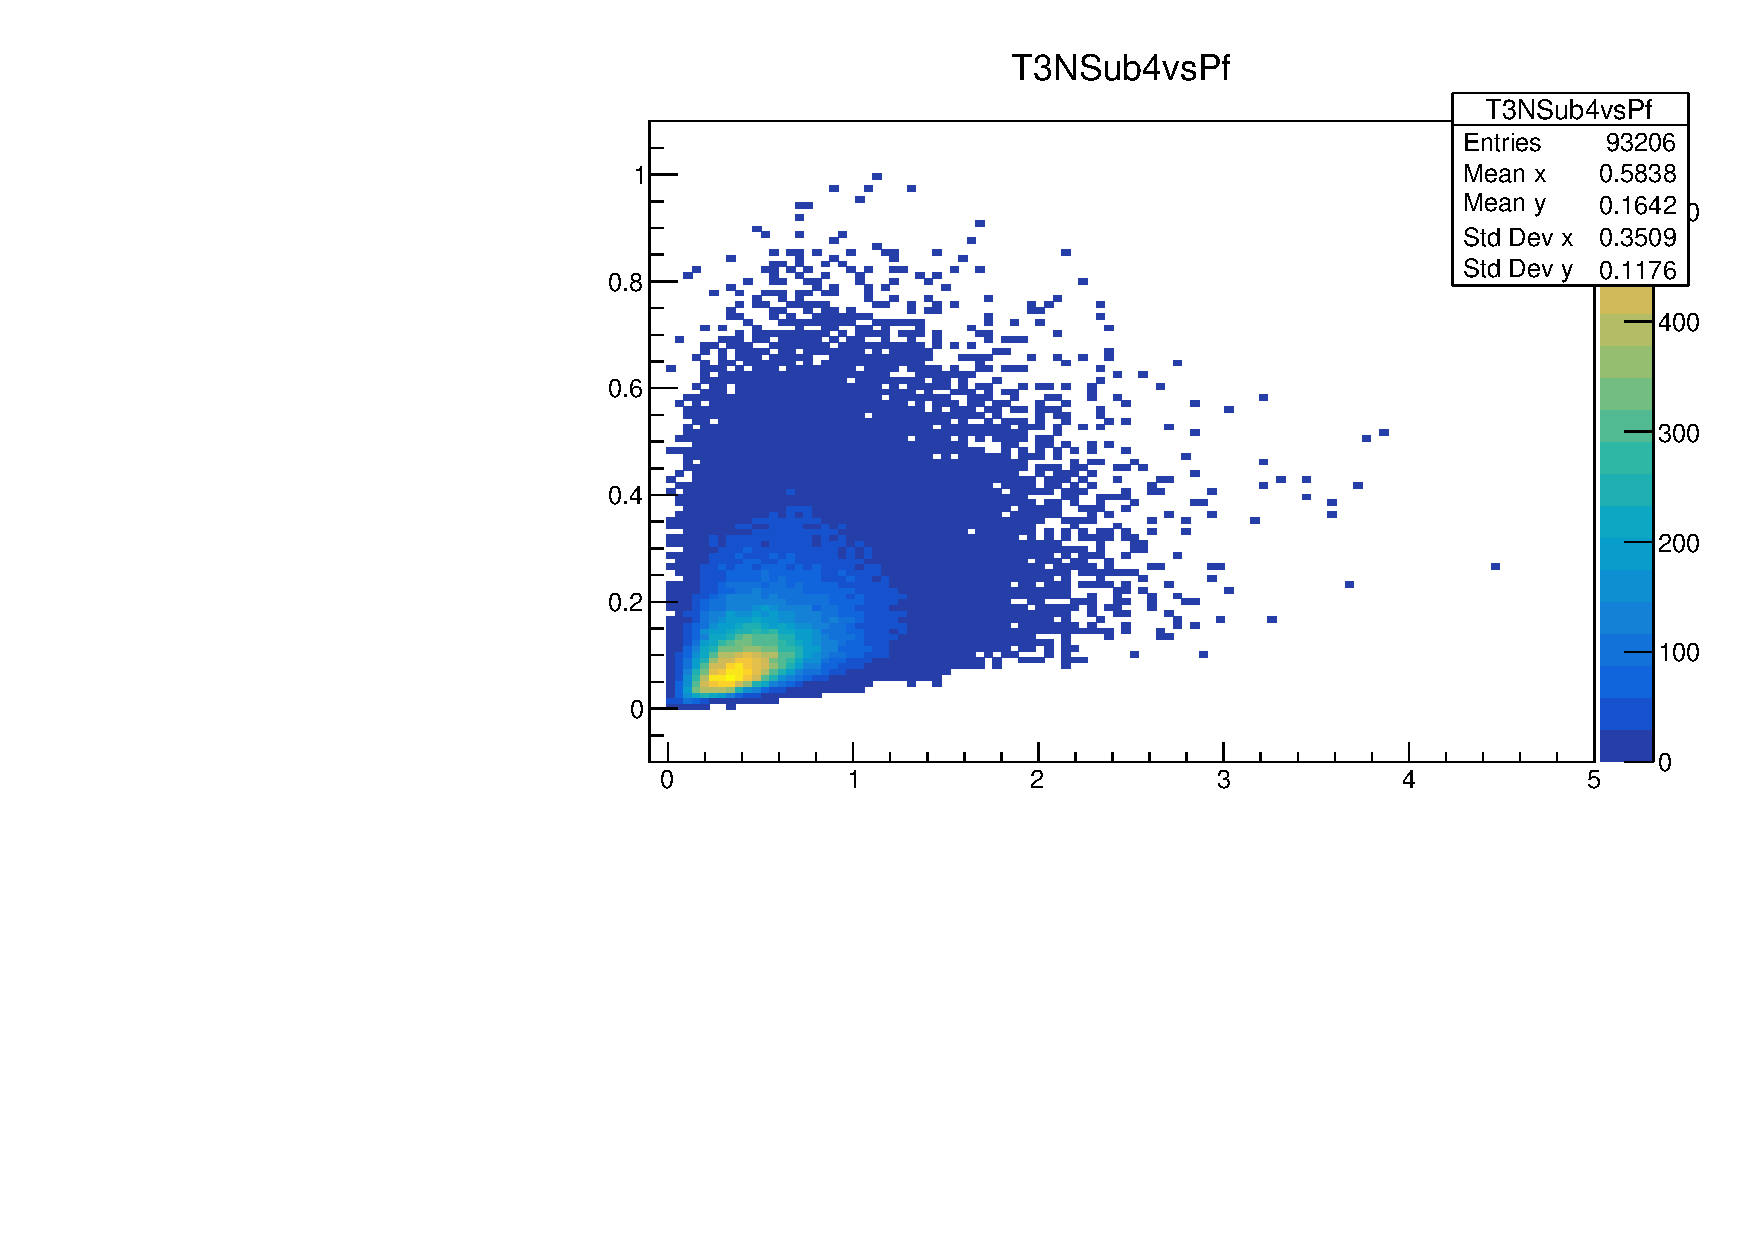
\includegraphics[width=0.49\textwidth]{./T3NSub4vsPf.pdf}\\
        \caption{ {\tt NSubjettiness} (x-axis) vs planar flow (y-axis) for boosted $jZ\rightarrow b \bar{b}$ }
        \label{fig:nsubvspf3}
    \end{center}
\end{figure}

\begin{figure}[H]
    \begin{center}
        \includegraphics[width=0.49\textwidth]{./T4NSub1vsPf.pdf}
        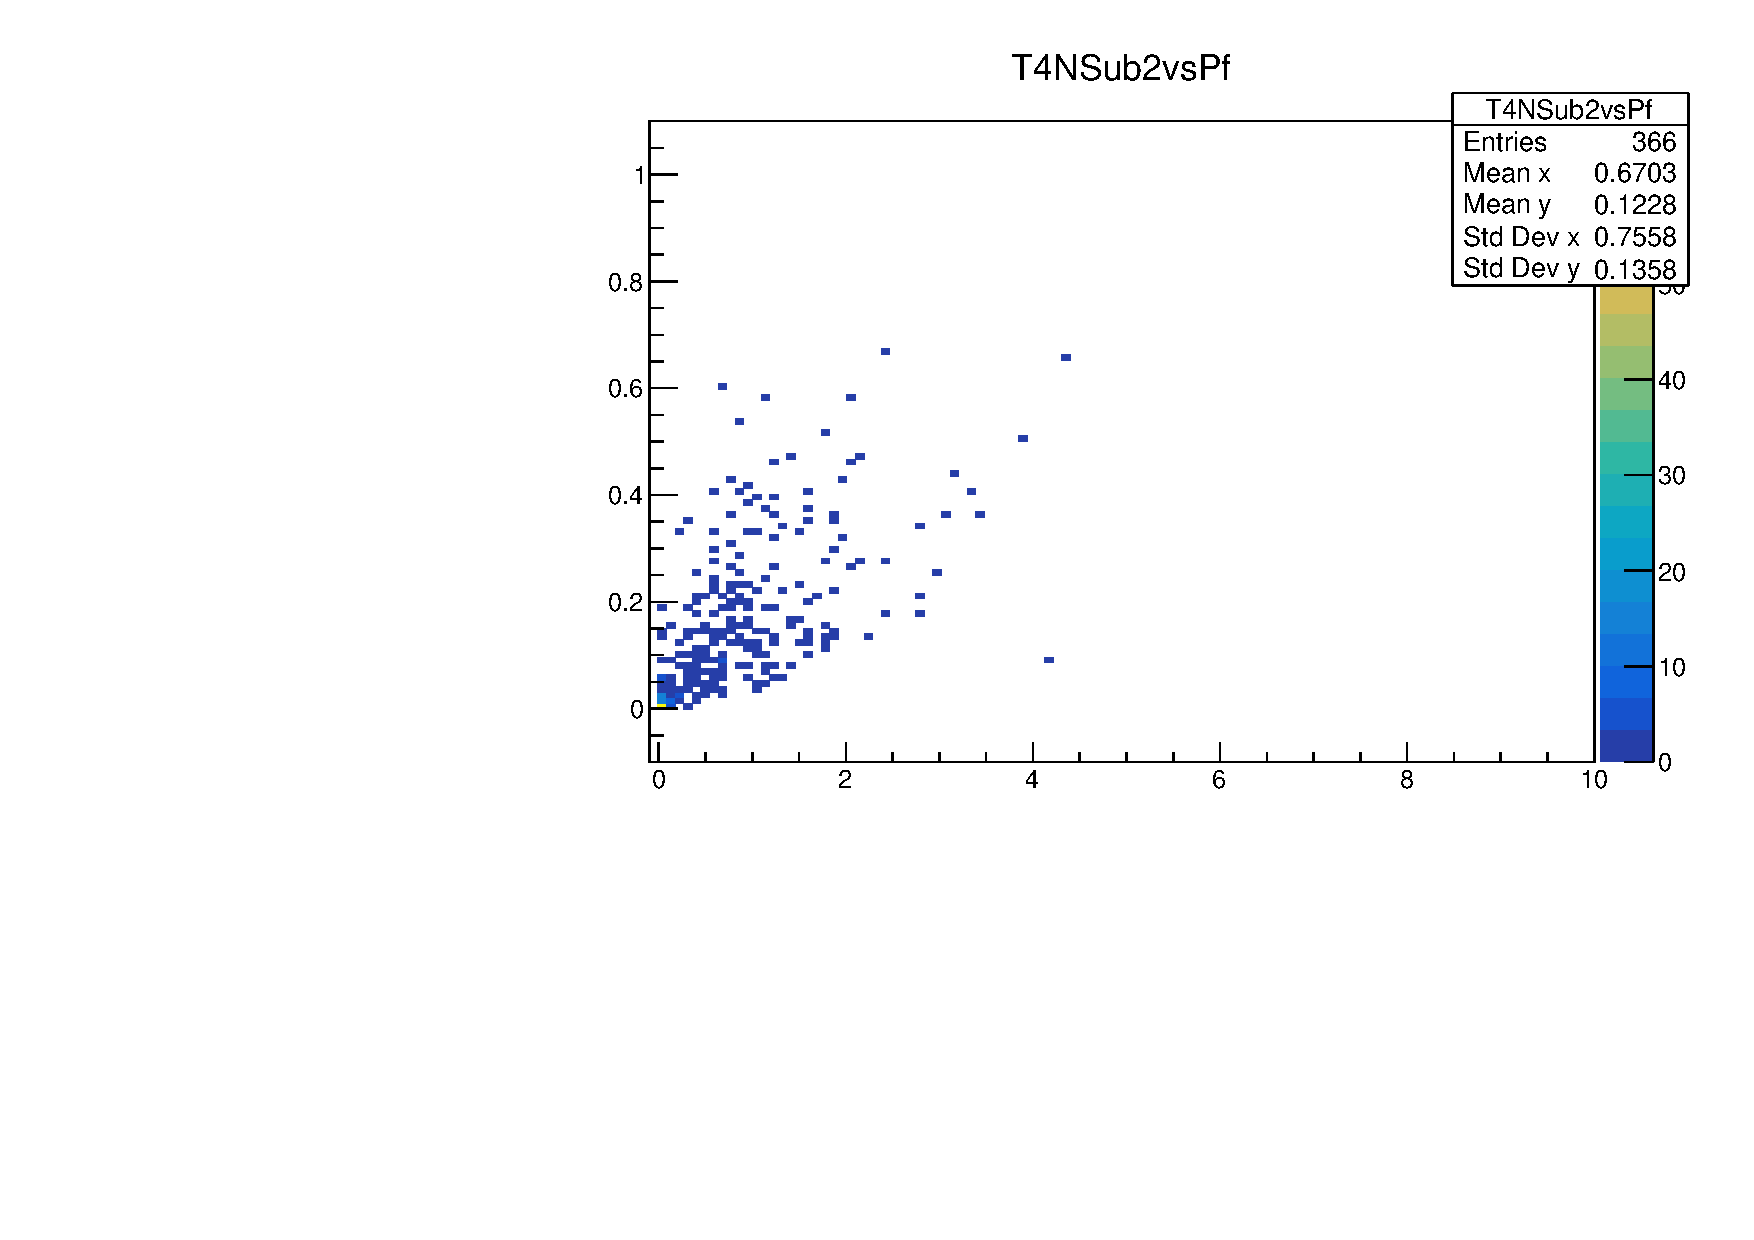
\includegraphics[width=0.49\textwidth]{./T4NSub2vsPf.pdf}\\
        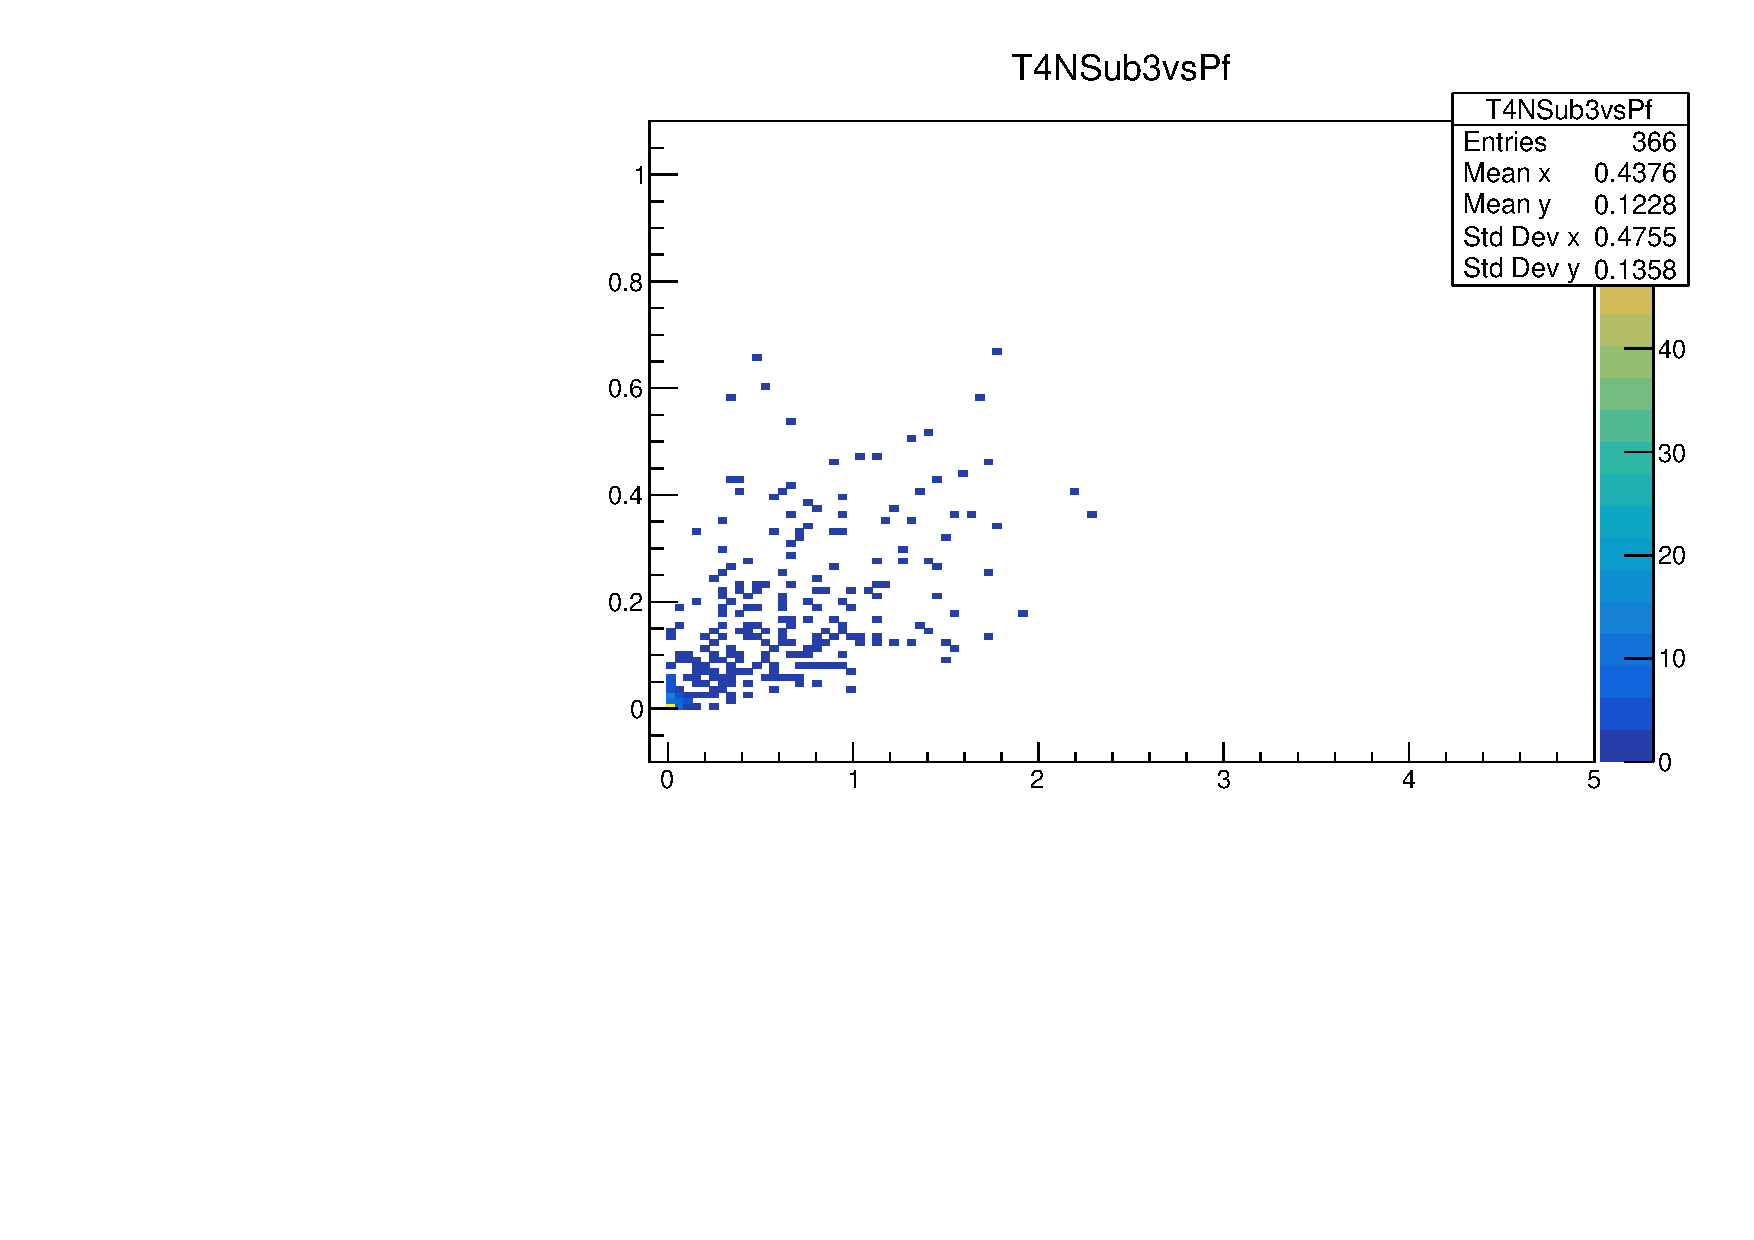
\includegraphics[width=0.49\textwidth]{./T4NSub3vsPf.pdf}
        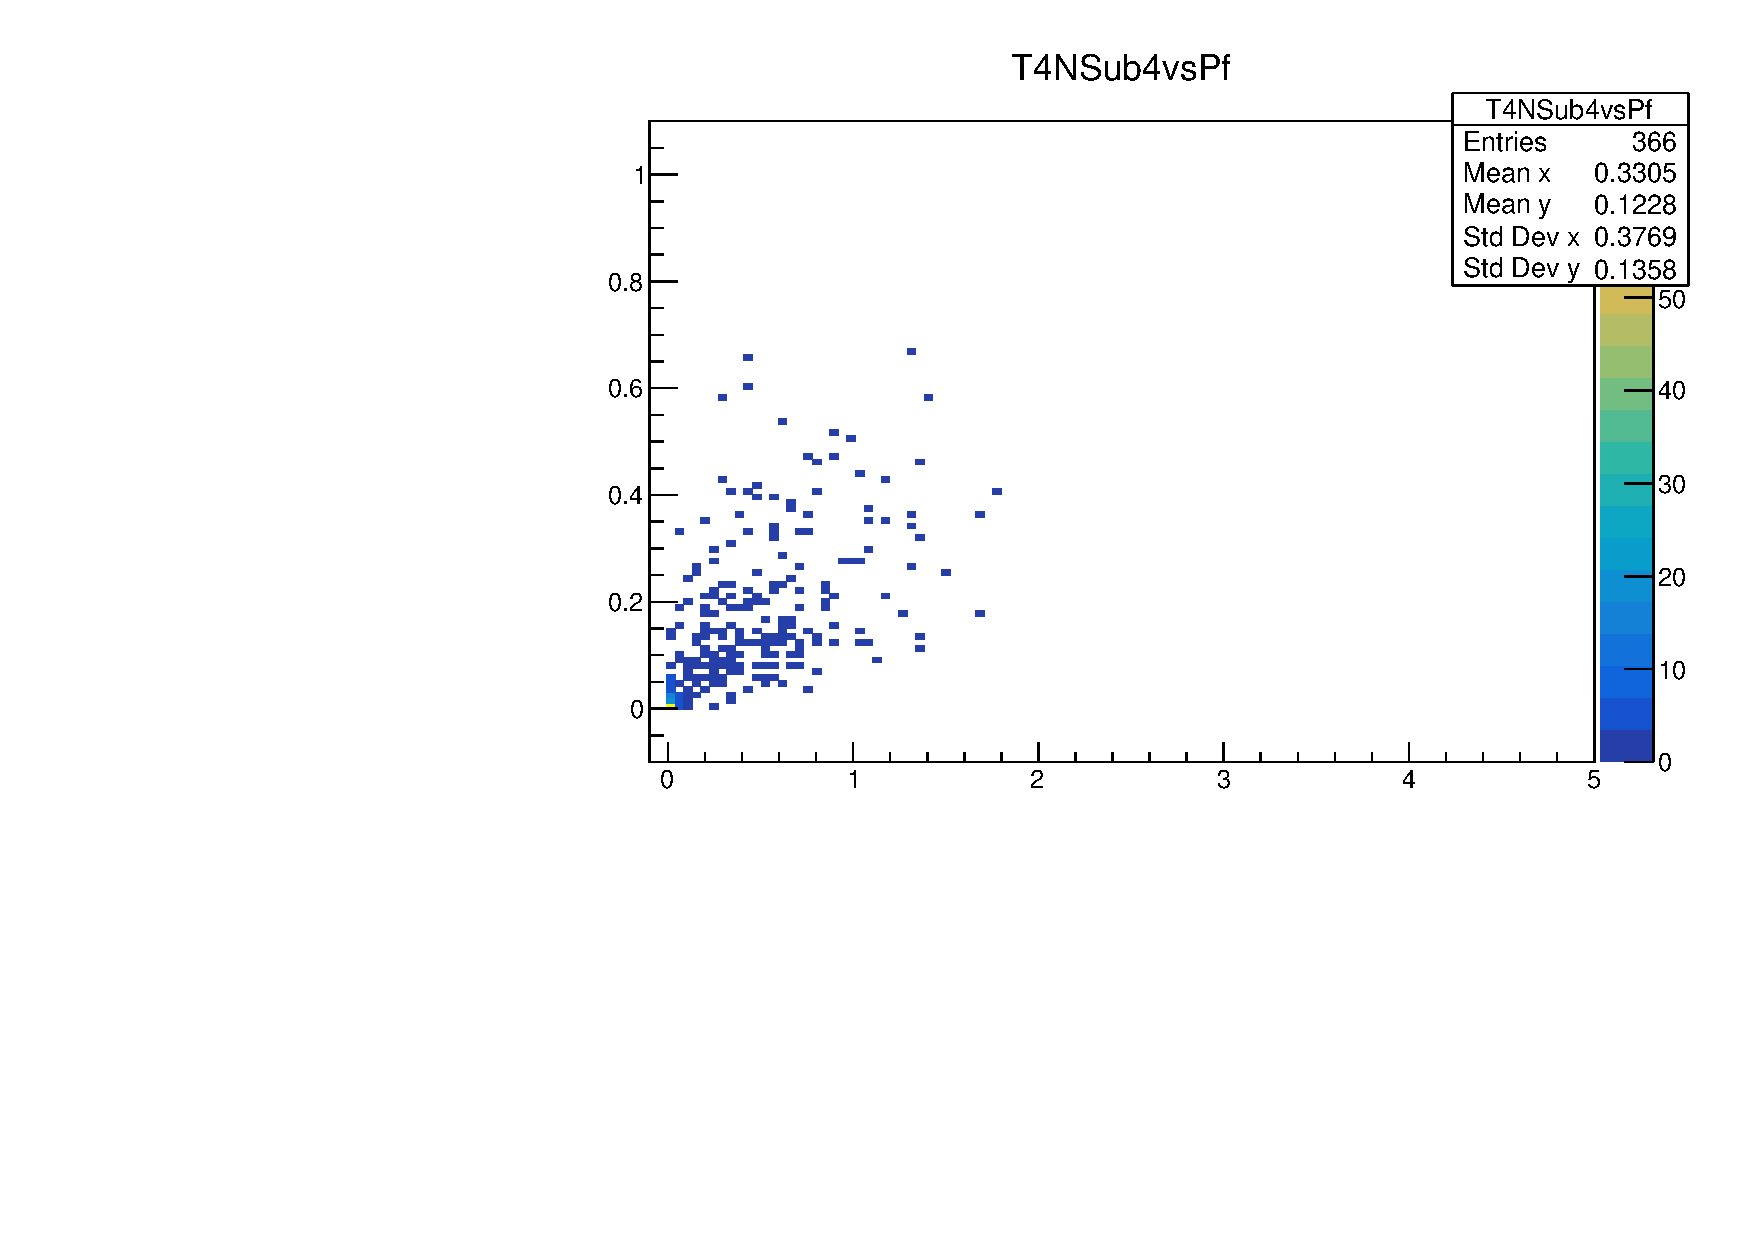
\includegraphics[width=0.49\textwidth]{./T4NSub4vsPf.pdf}\\
        \caption{ {\tt NSubjettiness} (x-axis) vs planar flow (y-axis) for unboosted $jZ\rightarrow \tau \bar{\tau}$ }
        \label{fig:nsubvspf4}
    \end{center}
\end{figure}

{\newpage}

\subsubsection{Analyzing planar flow:}

We suspect Planar Flow might be correlated with {\tt NSubjettiness}, to verify these, we check the following graphs [\autoref{fig:nsubvspf1},\autoref{fig:nsubvspf2},\autoref{fig:nsubvspf3},\autoref{fig:nsubvspf4}], as can be seen there seems to be some correlation, we quantify this:

\begin{eqnarray*}
    J & \equiv & \text{The }Z-\text{tagged jet obtained after BDRS + Filtering.}\\
    J_{1} & \equiv & \text{The highest }p_{T}\text{ subjet of }J.\\
    J_{2} & \equiv & \text{The other subjet of }J.\\
    P_{f} & \equiv & \text{Planar Flow}.\\
    \tau_{N} & \equiv & n^{th}\text{ NSubjettiness}.\\
    S\left(J\right) & \equiv & \sum_{i\in J}p_{T_{i}}\Delta R\left(i,J\right)\\
    \\
    \left\langle P_{f}\left(J\right),\tau_{2}\left(J\right)\right\rangle  & = & 3.70\times10^{-2}\\
    \left\langle P_{f}\left(J\right),\tau_{3}\left(J\right)\right\rangle  & = & 4.26\times10^{-2}\\
    \left\langle P_{f}\left(J\right),\tau_{4}\left(J\right)\right\rangle  & = & 4.32\times10^{-2}\\
    \left\langle P_{f}\left(J\right),\tau_{5}\left(J\right)\right\rangle  & = & 4.20\times10^{-2}\\
    \left\langle P_{f}\left(J\right),S\left(J\right)\right\rangle  & = & 9.73\times10^{-3}\\
    \\
    \left\langle P_{f}\left(J_{1}\right),\tau_{2}\left(J_{1}\right)\right\rangle  & = & 2.37\times10^{-1}\\
    \left\langle P_{f}\left(J_{1}\right),\tau_{3}\left(J_{1}\right)\right\rangle  & = & 2.37\times10^{-1}\\
    \left\langle P_{f}\left(J_{1}\right),\tau_{4}\left(J_{1}\right)\right\rangle  & = & 2.26\times10^{-1}\\
    \left\langle P_{f}\left(J_{1}\right),\tau_{5}\left(J_{1}\right)\right\rangle  & = & 2.15\times10^{-1}\\
    \left\langle P_{f}\left(J_{1}\right),S\left(J_{1}\right)\right\rangle  & = & 2.88\times10^{-1}\\
    \\
    \left\langle P_{f}\left(J_{2}\right),\tau_{2}\left(J_{2}\right)\right\rangle  & = & 2.32\times10^{-1}\\
    \left\langle P_{f}\left(J_{2}\right),\tau_{3}\left(J_{2}\right)\right\rangle  & = & 2.19\times10^{-1}\\
    \left\langle P_{f}\left(J_{2}\right),\tau_{4}\left(J_{2}\right)\right\rangle  & = & 2.00\times10^{-1}\\
    \left\langle P_{f}\left(J_{2}\right),\tau_{5}\left(J_{2}\right)\right\rangle  & = & 1.83\times10^{-1}\\
    \left\langle P_{f}\left(J_{2}\right),S\left(J_{2}\right)\right\rangle  & = & 2.72\times10^{-1}\\
\end{eqnarray*}

\begin{figure}[H]
    \begin{center}
        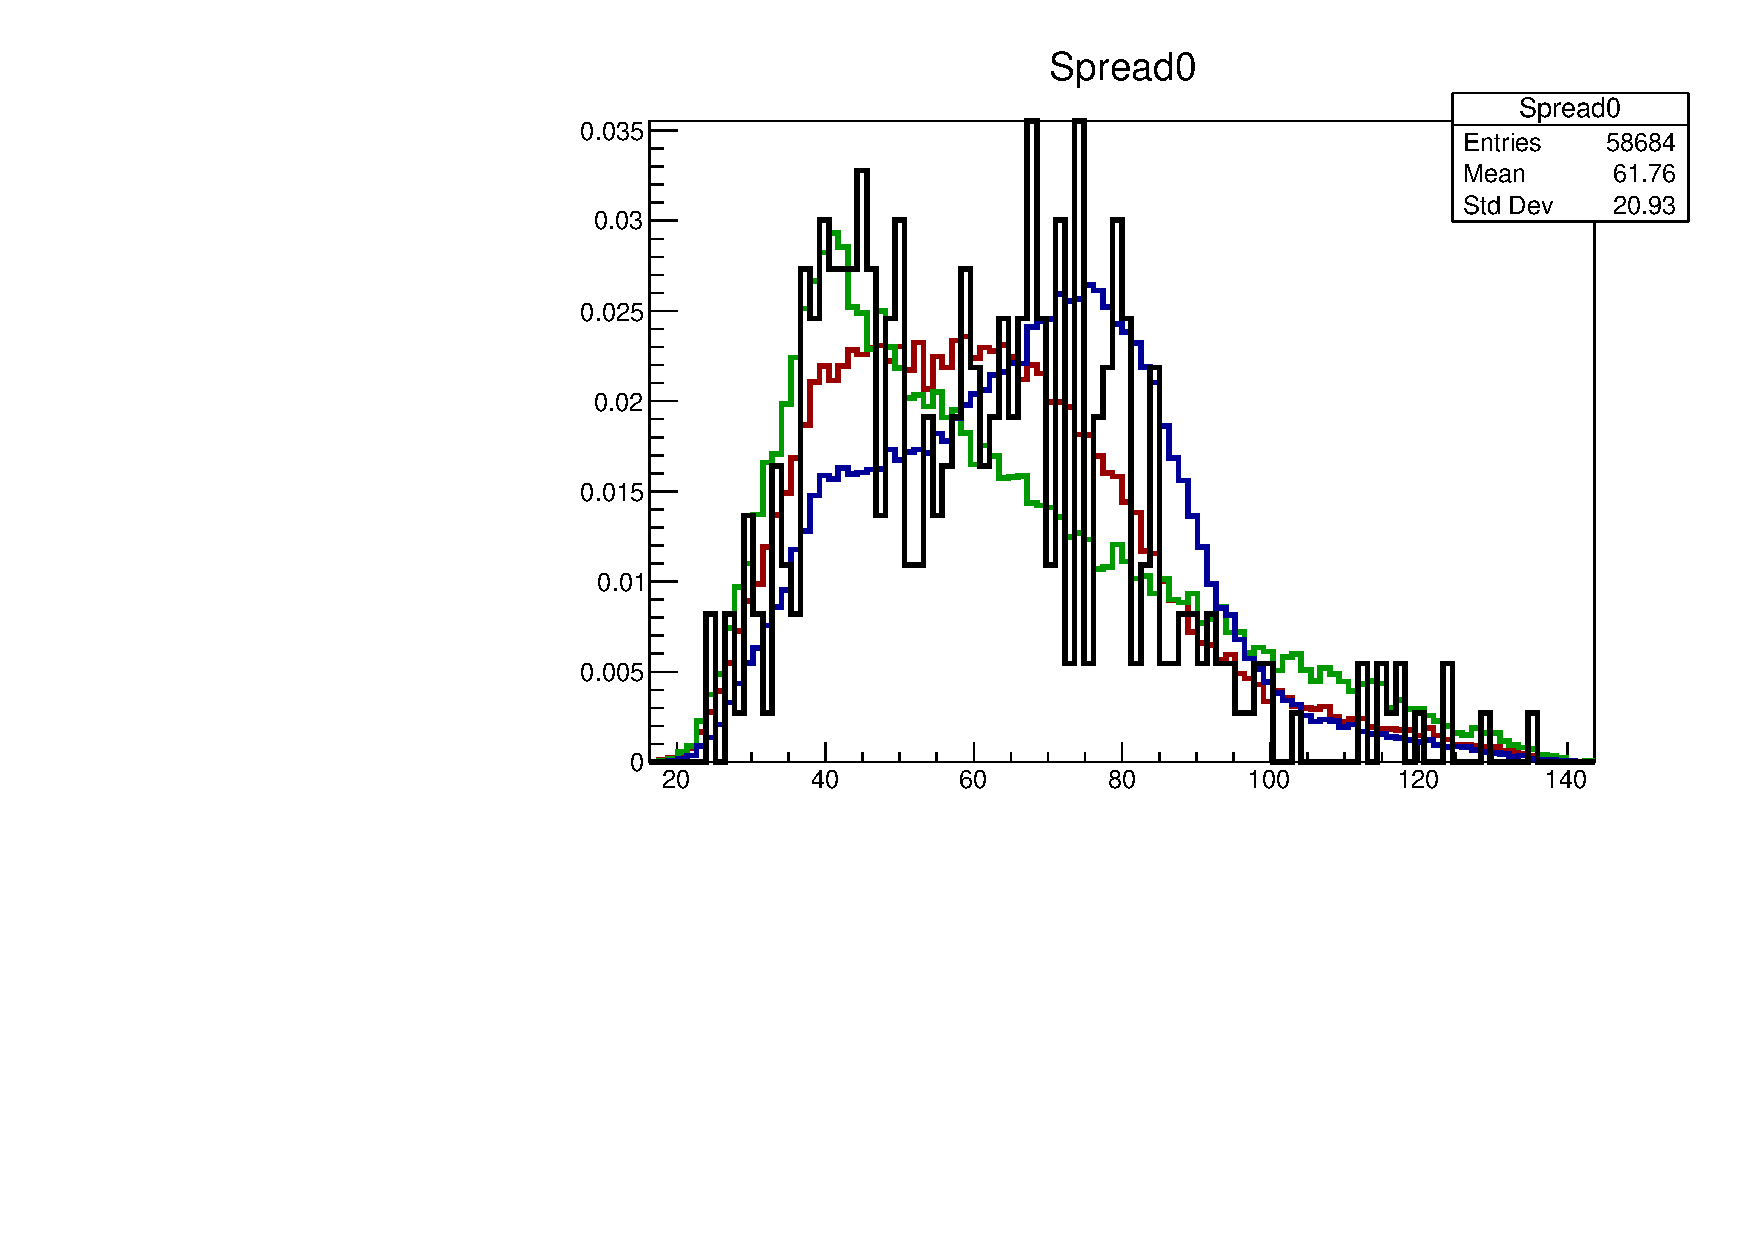
\includegraphics[width=0.7\textwidth]{./Spread0.pdf}
        \caption{ The variable $S\left(J\right)$  }
        \label{fig:Spread0}
    \end{center}
\end{figure}

\begin{figure}[H]
    \begin{center}
        \includegraphics[width=0.49\textwidth]{./Spread1.pdf}
        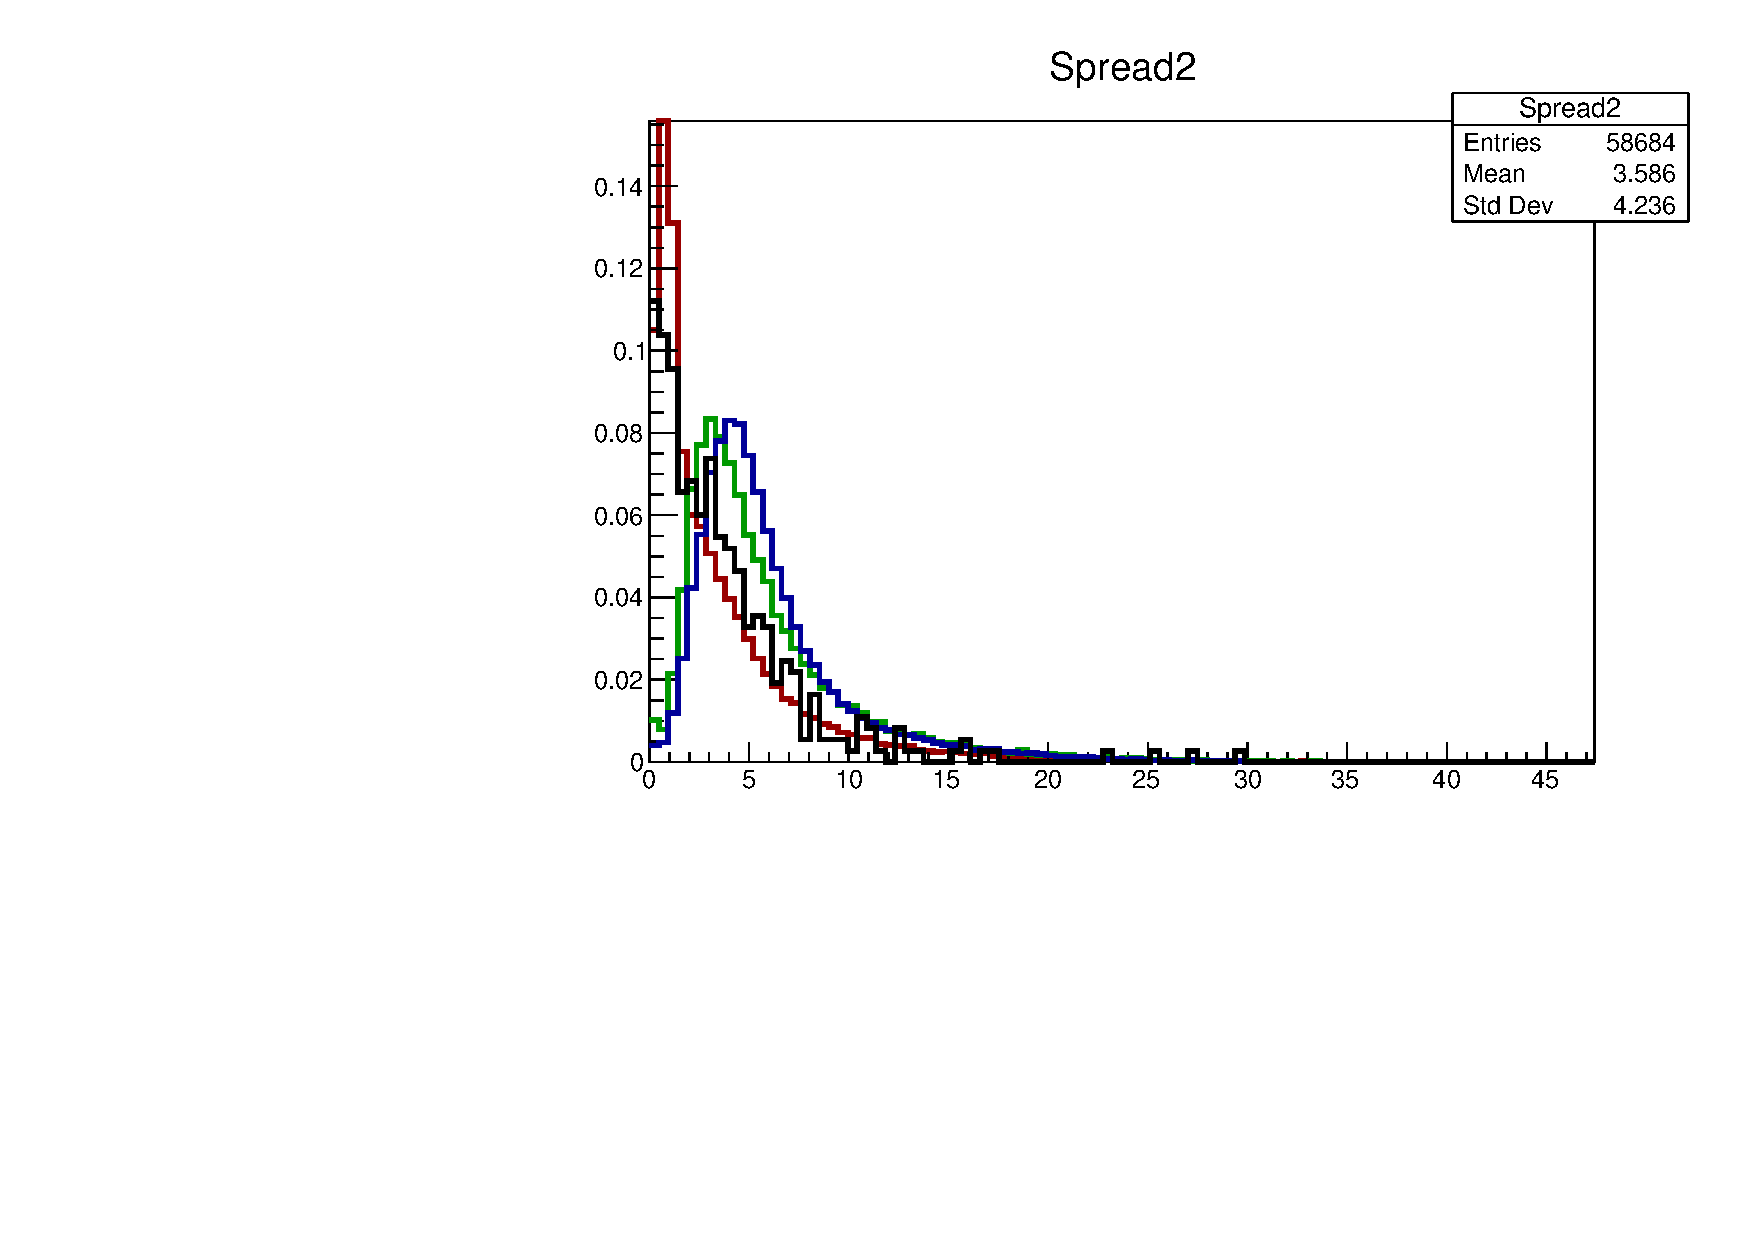
\includegraphics[width=0.49\textwidth]{Spread2.pdf}\\
        \caption{ The variable $S\left(J_1\right)$  and $S\left(J_2\right)$ }
        \label{fig:SpreadX}
    \end{center}
\end{figure}